%  
% Werktitel : Development of a technology file interface for SPACE
%
% Onderwerp : Ontwikkeling van een programma waarmee de technologie bestanden van SPACE
%             op een snelle manier gemaakt kunnen worden.
%
%
% Hoofdvraag: Wat zijn de belangrijkste problemen bij de ontwikkeling en hoe zijn deze opgelost?
%
% Achtergrondvragen:
%   - Wat is de omgeving waarin het programma is ontwikkeld?
%   - Welke ontwerpmethodes zijn toegepast?
%   - Waarom helpt dit programma bij de ontwikkeling van technologie bestanden? (Waarom optimaal)
%  
% Kernvragen:
%   - technische haalbaarheid
%   - flexibiliteit
%   - betrouwbaarheid
%
%
%
% Voorlopige inhoudsopgave
% -------------------------
% Titel
%   Development of a technology file interface for SPACE
% 
% Voorwoord    
%
% Samenvatting
%
% Inleiding
%
% Randvoorwaarden/wensen/eisen
%   - ontwikkelomgeving
% 
% ?? Systeemconcepten ??
%
% Uitwerking ontwerp
%
%   Use cases
%
%   Collaboration
%
%   The interface/generator specification language
%
% Testen
%
% Conclusie
%
%%%%%%%%%%%%%%%%%%%%%%%%%%%%%%%%%%%%%%%%%%%%%%%%%%%%%%%%%%%%%%%%%%%%%%%%%%%%%%
\documentclass[10pt,a4paper,twoside]{book}
% packages
\usepackage{graphicx}
\usepackage{fancyhdr}
\usepackage{alltt}
\usepackage{tabularx}
\usepackage{rotating}

% page header setup
\pagestyle{fancy}
\addtolength{\headheight}{\baselineskip}
%\renewcommand{\sectionmark}[1]{\markboth{\thesection.\ #1}{\thesection.\ #1}}

\renewcommand{\chaptermark}[1]{\markboth{\chaptername \ \thechapter.\ #1}{}}
\renewcommand{\sectionmark}[1]{\markright{\thesection.\ #1}}

%\lhead{\leftmark\\\rightmark}
%\rhead{\thepage}

\cfoot{}
%%%%%%%%\renewcommand{\sectionmark}[1]{\markboth{\thesection.\ #1}{\thesection.\ #1}}
%%%%%%%%%%\renewcommand{\sectionmark}[1]{\markright{\thesection.\ #1}}
%%%%%%%%%%\renewcommand{
%%%%%%%%\fancyhead[R]{\thepage}
%%%%%%%%\fancyhead[L]{\rightmark}

\fancypagestyle{plain}{%
\fancyhf{}
\fancyhead[RO,LE]{\thepage} \renewcommand{\headrulewidth}{0pt} 
\fancyhead[LO,RE]{\renewcommand{\headrulewidth}{0pt} }
%\fancyhead[]{\thepage} \renewcommand{\headrulewidth}{0pt}
} 


% Environments used in the language reference sections of the language chapter:
\newenvironment{PropTable}[1][Supported properties:]
{
    \par \bigskip \noindent {#1}\\
    \begin{tabular}{l|p{8cm}}
    \hline
     \textsf{Property}  & \textsf{Description} \\
    \hline
}
{\\ \hline \end{tabular}}

% This is from Nick, for the big table in the language.tex file.
\newcounter{act}
\newcommand{\R}[1]{\ref{a#1}}
\newcommand{\actd}[1]{\refstepcounter{act}\label{a#1}}
\newcommand{\rotated}[1]{\begin{sideways}#1\end{sideways}}
\newcommand{\TabCap}[1]{\multicolumn{1}{|l|}{\begin{sideways}\texttt{#1}\end{sideways}}}
\newcommand{\TR}[2][]{\R{#2} #1}

% titlepage stuff
%\title{Design and implementation of a technology file interface for SPACE}
%\author{Xander Burgerhout \\ Delft University of Technology \\ CAS report nr.: N\&S-A-2003 (pre-release)}
%\date{November 2000}

% Sloppy.
\sloppy

%%%%%%%%%%%%%%%%%%%%%%%%%%%%%%%%%%%%%%%%%%%%%%%%%%%%%%%%%%%%%%%%%%%%%%%%%%%%%%
\begin{document}

% front matter
%\maketitle
\fancyhf{}
%\fancyhead[LE,RO]{\thepage \renewcommand{\headrulewidth}{0pt}}
%\fancyhead[RE,LO]{\renewcommand{\headrulewidth}{0pt}}

\newlength{\centeroffset}
\setlength{\centeroffset}{-0.5\oddsidemargin}
\addtolength{\centeroffset}{0.5\evensidemargin}

\thispagestyle{empty}
\vspace*{\stretch{0.1}}

\noindent\hspace*{\centeroffset}\makebox[0pt][l]{\begin{minipage}{\textwidth}
    \center{
        \noindent\rule[-1ex]{\textwidth}{2pt}\\[2.5ex]
            \LARGE{\bfseries
                Design and implementation \\
                of a  technology file \\
                interface for SPACE}
        \noindent\rule[0ex]{\textwidth}{2pt}\\[2.5ex]
    }
    \hfill\emph{\large Xander Burgerhout}
    \end{minipage}
}

\vspace{\stretch{0.3}}

\noindent\hspace*{\centeroffset}\makebox[0pt][l]{\begin{minipage}{\textwidth}
    \center{
        \emph{
            Circuits and Systems group\\
                Department of Electrical Engineering\\
                Delft University of Technology\\
                Mekelweg 4, 2628 CD Delft\\
                The Netherlands}}
    \end{minipage}
}

\vspace{\stretch{2}}

\noindent\hspace*{\centeroffset}\makebox[0pt][l]{\begin{minipage}{\textwidth}
    \flushleft{
        \small{
        \begin{tabular}{ll}
            Delft, January 21, 2001 & \\
            Technical Report no. & : N\&S-A-2003\\
            Mentor & : dr. ir. N. P. van der Meijs\\
             & \\
           \end{tabular}
        }
    }
    \begin{center}
    
\includegraphics[width=0.25\textwidth]{./figures/TUcolorlogo.eps}\\
    {\scriptsize Delft University of Technology}
    \end{center}

    \end{minipage}
}

\pagebreak



\frontmatter
% preface.tex

\chapter*{Preface}
\label{chap:preface}
\addcontentsline{toc}{chapter}{Preface}

This report and the application it describes is the result of a graduation
project. This graduation project has been performed for (and at) the Circuits
and Sytems group which is part of the faculty of Electrical Engineering at
Delft University of Technology.

Two important parts of this report are the design and implementation of the
architecture and a sort of a reference guide to the configuration file
language. Readers interested in the architecture of the application should read
at least Chapter \ref{chap:design}. Those more interested in the configuration
file language are referred to Chapter \ref{chap:language}.

Finally, I would like to thank dr. ir. Nick van der Meijs for his guidance,
opinions and advice during the project.

\bigskip \bigskip \noindent
Delft, January 2001 \hfill X.B.


\lhead{\leftmark}
\tableofcontents
\mainmatter

\fancyhf{}
\fancyhead[LE,RO]{\thepage}
\fancyhead[LO,RE]{}

% abstract.tex

\chapter*{Abstract}
\addcontentsline{toc}{chapter}{Abstract}
The current version of the layout-to-circuit extractor SPACE does not have a
user friendly interface to add new process descriptions or change existing
descriptions. This is currently a specialized job.

\bigskip \noindent
This report describes the design and implementation of a user-friendly tool
that can be used to add and manage the technology files that describe a
process.

\bigskip \noindent
Flexibility is an important requirement. It must be possible to easily add new
technology files to the interface. Another important requirement is platform
independence. It must be possible to use the platform on many different flavors
of Unix.

\bigskip \noindent
To meet the demand of flexibility the application uses a configuration file in
which the user interface and the format of the technology files is specified.
The developed application uses the information in the configuration file to
create a user interface and to generate the required technology files.

A parser has been created that can read the configuration file and build a
graphical user interface from the information it encounters. The values entered
by the user into this user interface are then used by the generators specified
in the configuration file to generate the requested technology files.

\bigskip \noindent
The Qt toolkit from TrollTech ensures platform independence of the graphical
user interface. This popular toolkit is available for many types of Unix,
Linux, Windows and even for embedded environments.

\listoffigures
\listoftables


% The chapters
\fancyhead[LO,RE]{\rightmark}
%% Introduction
%%
% Onderwerp : Ontwikkeling van een programma waarmee de technologie bestanden van SPACE
%             op een snelle manier gemaakt kunnen worden.
%
%
% Hoofdvraag: Wat zijn de belangrijkste problemen bij de ontwikkeling en hoe zijn deze opgelost?
%
% Achtergrondvragen:
%   - Wat is de omgeving waarin het programma is ontwikkeld?
%   - Welke ontwerpmethodes zijn toegepast?
%   - Waarom helpt dit programma bij de ontwikkeling van technologie bestanden? (Waarom optimaal)
%  
% Kernvragen:
%   - technische haalbaarheid
%   - flexibiliteit
%   - betrouwbaarheid
%%%%%%%%%%%%%%%%%%%%%%%%%%%%%%%%%%%%%%%%%%%%%%%%%%%%%%%%%%%%%%%%%%%%%%%%%%%%%%

\chapter{Introduction}
\label{chap:introduction}

A layout-to-circuit extractor like SPACE\footnote{\emph{SPACE} is the 
layout--to--circuit extractor developed at the Circuits and Systems group of 
the Electrical Engineering faculty. SPACE has been quite successful so far. It 
is used by several companies and universities, including Agilent (Hewlett 
Packard) and Level One (Intel).}  must (of course) be able to handle all kinds 
of processes. In SPACE, each of these processes is described by a set of 
\emph{technology files}. The contents of these files vary from simple layer 
specification to complex capacitance tables.

Until now, the technology files were maintained by hand. This means that for 
each process all the technology files had to be entered manually, a 
time-consuming and error-prone task. Also, the user must be familiar with the 
file format of each of the technology files, which makes process entry and 
maintenance a specialized task.

\emph{SPOCK} is to alleviate the problems described above by presenting the 
user with a graphical user interface in which the required data can be entered.

\bigskip \noindent
The main goal of this thesis is to identify the problems encountered during 
the design and implementation of SPOCK and to describe the solutions that were 
used to solve these problems.

\bigskip \noindent
Chapter \ref{chap:demands} presents the demanded functionality of the 
application as well as some imposed constraints. Chapter \ref{chap:design} 
discusses and explains the final design. The user interface plays an important 
role in this application. Some standard and custom user interface elements are 
therefore presented in Chapter \ref{chap:uidesign}. Chapter 
\ref{chap:language} describes the configuration file language. As will become 
clear later, the configuration file describes the technology files supported 
by the application.
%Chapter \ref{chap:environment}) describes the tools used during development. Some 
%comments on the testing and debugging process will be given in Chapter 
%\ref{chap:testing}. 
The final chapter will contain some concluding remarks.

% demands.tex
%%%%%%%%%%%%%%%%%%%%%%%%%%%%%%%%%%%%%%%%%%%%%%%%%%%%%%%%%%%%%%%%%%%%%%%%%%%%%%

\chapter{Application requirements}
\label{chap:demands}

%%%%%%%%%%%%%%%%%%%%%%%%%%%%%%%%%%%%%%%%%%%%%%%%%%%%%%%%%%%%%%%%%%%%%%%%%%%%%%
%\section{Introduction}
As a first step in the design process, the demands and constraints for the
application must be charted. In this chapter the most important demands and
constraints are given.

Firstly, the constraints resulting from the environment in which the
application must function are enumerated in Section
\ref{sect:demands:environment}). Secondly, the functional demands are listed in
Section \ref{sect:demands:functional}. Documentation is also important: demands
related to documentation can be found in Section
\ref{sect:demands:documentation}. Some general wishes are mentioned in Section
\ref{sect:demands:wishes}.

%%%%%%%%%%%%%%%%%%%%%%%%%%%%%%%%%%%%%%%%%%%%%%%%%%%%%%%%%%%%%%%%%%%%%%%%%%%%%%
\section{Application environment constraints}
\label{sect:demands:environment}
\subsection{Platform}
It must be possible to compile the application on various platforms since SPACE
can also be compiled on various platforms. The following platforms must be
supported:
\begin{itemize}
\item Solaris
\item HP UX
\item Linux
\end{itemize}
Any input and/or output files that are read or written by the application must
also be platform independent. This means for example, that it must be possible
to read a file saved with the Solaris version into the Linux version and
vice-versa.

\subsection{Integration}
The application must integrate correctly with the rest of the SPACE package.
This mainly means that the application should honor the directory structure and
the environment settings used by SPACE.

%%%%%%%%%%%%%%%%%%%%%%%%%%%%%%%%%%%%%%%%%%%%%%%%%%%%%%%%%%%%%%%%%%%%%%%%%%%%%%
\section{Functional demands}
\label{sect:demands:functional}
\subsection{Technology file generation}
It should be possible to generate technology files with a plain-text file
format. There must also be a mechanism that will allow the addition (or
removal) of technology file formats. As a proof of concept the application must
be able to generate the following subset of technology files:
\begin{itemize}
\item \emph{maskdata}, which defines the layers present in the process and the
colors used to represent them in the programs and their output.
\item \emph{space.xxx.s}, the element definition files used by SPACE.
\item \emph{space.xxx.p}, the parameter files used by space.
\item \emph{bmlist.gds}, which provides a mapping between the GDS layer format and
the format used by SPACE.
\item \emph{xspicerc}, a control file that specifies which models are used for
the devices.
\end{itemize}

\subsection{Flexibility}
Flexibility is very important. Recompilations as a result of adding, changing
or removing a technology file format should be kept to a minimum to decrease
the maintenance cost of the application.

%%%%%%%%%%%%%%%%%%%%%%%%%%%%%%%%%%%%%%%%%%%%%%%%%%%%%%%%%%%%%%%%%%%%%%%%%%%%%%
\section{Documentation demands}
\label{sect:demands:documentation}
The following documentation must be created:
\begin{itemize}
\item Source code documentation
\item Installation manual
\item Programmers manual
\item Maintainers manual
\end{itemize}

%%%%%%%%%%%%%%%%%%%%%%%%%%%%%%%%%%%%%%%%%%%%%%%%%%%%%%%%%%%%%%%%%%%%%%%%%%%%%%
\section{Additional wishes}
\label{sect:demands:wishes}
The user interface must be consequent and consistent. This means the user
interface should conform to the currently accepted standard.

A ``help'' facility would be welcomed. It should at least be possible to show
``tooltips'' (popup hints).

\bigskip \noindent
If possible, the application will be implemented in C++.

% design.tex

\chapter{Design and implementation}
\label{chap:design}

%%%%%%%%%%%%%%%%%%%%%%%%%%%%%%%%%%%%%%%%%%%%%%%%%%%%%%%%%%%%%%%%%%%%%%%%%%%%%
%\section{Introduction}
Designing and implementing is often an iterative process. No matter how
detailed your design is, chances are that you will still encounter problems
during implementation that will require a design change. In this chapter,
design and implementation issues are therefore presented together.

\bigskip \noindent
The main goal of this chapter is to present the entire design and the related
implementation issues and choices.

\bigskip \noindent
In the first section (\mbox{Section \ref{sect:design:architecture}}) of this
chapter the architecture of the application will be presented. Next, the
architecture of the user interface will be explained. This will not include the
user interface elements (see Chapter \ref{chap:uidesign} for that) but will be
about the organization of the user interface. The main parts of the design will
be explained in detail in Section \ref{sect:design:parser} to Section
\ref{sect:design:serialization}.

Before the chapter is concluded some recommendations for future extensions are
given in Section \ref{sect:design:future}. A graphical overview of the
implemented design can be found in the final section of this chapter.

%%%%%%%%%%%%%%%%%%%%%%%%%%%%%%%%%%%%%%%%%%%%%%%%%%%%%%%%%%%%%%%%%%%%%%%%%%%%%
\section{Application architecture} \label{sect:design:architecture}
First, the problems related to a traditional architecture are discussed. Next,
a solution to these problems is presented.

\subsection{The problem} \label{sect:design:problem}
The main function of the application can be described quite easily. The user
enters data into the application in a user-friendly way. The application then
takes this data and generates the more complex files needed by SPACE. This
means the user interface and the data are strongly related.

The traditional way to implement this kind of application is to use a rapid
application development (RAD) tool like X-designer\footnote{X-designer allows a
programmer to visually create a user interface based on Motif. More information
on X-designer can be found on \texttt{http://www.ist.co.uk}.} or
Qt-designer\footnote{Qt-designer allows a programmer to visually create a user
interface based on the Qt toolkit. More information can be found on the
Qt-designer section of TrollTech \cite{Qt}
\texttt{http://www.trolltech.com/products/qt/designer/index.html}.}. The user
interface can visually be created with these applications.

As was mentioned before, flexibility is a very strong demand. Recompilations
resulting from the actions listed below should be kept to a minimum:
\begin{itemize}
\item make changes to existing files
\item add new files to the generation process
\item remove files from the generation process
\end{itemize}
This requirement has some consequences though. In these cases, using a tool
like X-designer or Qt-designer has the following disadvantages:
\begin{itemize}
    \item A change in the file format of one of the technology files to be
    generated requires changes to the user interface. This means that source
    code has to be changed manually or be regenerated when using tools like
    X-Designer or Qt-Designer.
    \item A recompilation is always necessary. Even if the user interface can
    be left unchanged, at least the generating algorithm must be updated.
    \item User interface and file generation information is distributed over
    many files, making maintenance non-trivial.
\end{itemize}
Recompilation as a result of a change in the format of one of the files to be
generated would dramatically increase the maintenance costs required by the
application, so a solution should be found for the problems mentioned above.

The second problem mentioned in the list above can be avoided by using a file
which specifies the generation algorithm. This is useful in the case that only
the format of a technology file changes. It hardly reduces the need for a
recompilation however. A change in the format of a technology file (new
features e.g.) is far more likely to occur than a change in the generating
algorithm. It also does not solve the problem of adding files to the generation
process.

\bigskip \noindent
RAD tools like X-designer and Qt-designer speed up the development of the user
interface and introduce a certain flexibility. However, in this case they do
not introduce enough flexibility, because a recompilation is still very likely
to be needed in the case of adding, removing or changing technology file
formats. The approach presented in the next section does not have these
disadvantages.

\subsection{The solution} \label{sect:design:solution}
To solve the problems mentioned in the previous section we need a different
approach. Instead of using a design tool like X-designer or Qt-designer, we can
use a configuration file.

The configuration file will describe the user interface, the technology file
format descriptions and the relationship between them. This configuration file
will then be parsed by the application. This approach has the advantages we are
looking for:
\begin{itemize}
\item Adding, removing or changing a technology file format no longer results
in the need for a recompilation of the application. Only the configuration file
needs to be updated.
\item The user interface and technology file format descriptions are contained in one file.
This means that maintenance is also limited to one file.
\end{itemize}
The next (sub)section will give a general overview of the resulting
architecture.

\subsection{General overview} \label{sect:design:overview}
The solution as presented in Section \ref{sect:design:solution} leads to the
architecture presented in \mbox{Figure \ref{fig:design:overview}}.
\begin{figure}
\begin{center}
    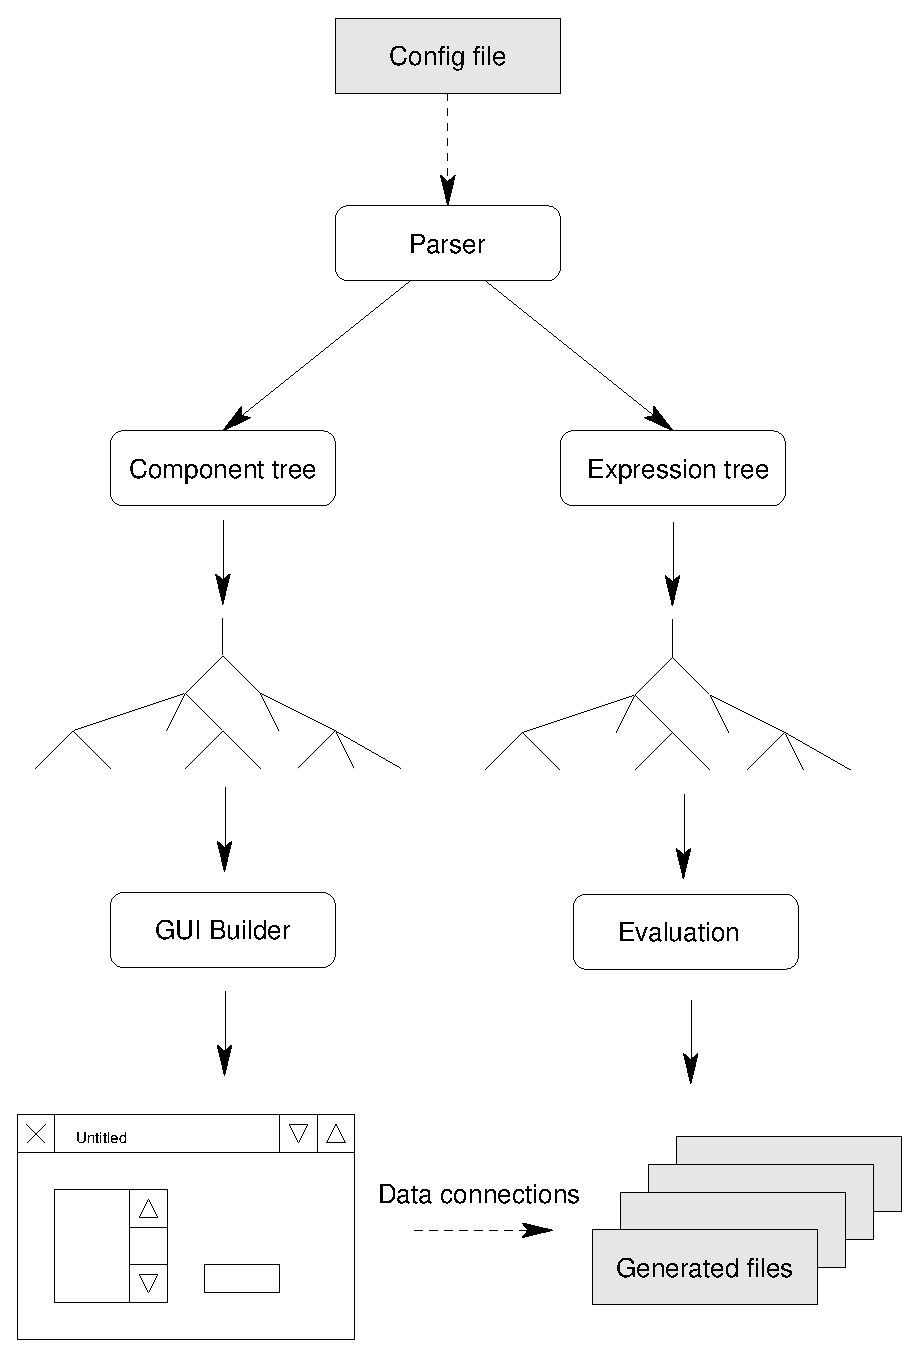
\includegraphics[width=9cm]{./figures/app_overview_new.eps}
    \caption{General view of how the application performs its task}
    \label{fig:design:overview}
\end{center} \end{figure}
The main function of the application --- generating files based on some
configuration and the users input --- is quite clear in this picture. The
entire process can be summarized as follows:
\begin{itemize}
\item Read and parse the configuration file containing a user interface
description and technology file format specifications.
\item Build the the technology file generators and build the user
interface using a ``component tree''.
\item Use the generators and the data entered in the user interface to generate
the required files.
\end{itemize}
First, the configuration file is read. The configuration file contains a
description of the user interface as well as information on how to generate the
required technology files. The user interface description actually specifies
\emph{what} data the user must enter and also \emph{how} the user must do this.
The technology file generator specification contains literal pieces of files as
well as references to elements in the user interface that will be substituted
with entered values. For more information on the format of this file see
\mbox{Chapter \ref{chap:language}}.

To efficiently build the user interface, a component tree is first created.
This component tree is then used to build the actual Qt
widgets\footnote{Widgets are the basic elements a user interface consists of,
e.g. buttons, listboxes, checkboxes, etc.}. A precise description of this
process can be found in \mbox{section \ref{sect:design:uibuilder}}.

The last step is file generation. To be able to generate the technology files,
data is collected from the user interface and fed into the file generators,
resulting in the required files.

%%%%%%%%%%%%%%%%%%%%%%%%%%%%%%%%%%%%%%%%%%%%%%%%%%%%%%%%%%%%%%%%%%%%%%%%%%%%%
\section{User interface architecture} \label{sect:design:ui_architecture}
The user interface can be separated into two parts. The first part handles
opening and closing files and file generation requests. It also provides an
interface for the second part. This first part will be called the
``framework''.

The second part of the user interface is the part of the user interface that is
described in the configuration file. This part specifies what data must be
entered (and how) to be able to generate a certain file. This second part will
be called the generated user interface.

%Since this is open to change we cannot be as specific as for the framework.

\subsection{The framework}
The framework used is just an implementation of the well-known multiple
document interface (MDI). The framework provides the actions the user expects
to find in a multiple document interface:
\begin{itemize}
\item Creating a new file
\item Opening (loading) of a file
\item Saving of a file
\item Closing of a file
\item Switching between open files
\end{itemize}
If we translate this abstraction to our case, the ``file'' is a process
description. Switching between files means that the user would like to start
editing on another process. The actions provided are grouped together in the
``File'' menu, as is common practice. The interested reader is referred to an
excellent book on user interface standards by Fowler and Stanwick
\cite{Fowler}.

\begin{table}[b] \begin{center}
\caption{Partial list of methods provided by the CProcessManager class.}
\label{tab:design:CProcessManager}
\begin{tabular}{l|p{6cm}}
\hline
 \textsf{Method}   & \textsf{Description}                                               \\
\hline
 \verb=currentProcess()=  & Gives a pointer to the process currently being edited by the user. \\
 \verb=newProcess()=      & Creates a new process and makes it the current process.            \\
 \verb=activateProcess()= & Switches to a new process.                                         \\
 \verb=removeProcess()=   & Closes and removes the process from the process manager.           \\
 \verb=saveProcess()=     & Saves a process to disk.                                           \\
 \verb=loadProcess()=     & Loads a process from disk.                                         \\
 \verb=generateFile()=    & Generates the requested technology file for this process.          \\
\hline
\end{tabular}
\end{center} \end{table}

In the implementation, the multiple document interface can mainly be found in
three classes: \verb=CAppMainWindow=, \verb=CProcessManager= and
\verb=CProcess=. The \linebreak \verb=CAppMainWindow= class receives the
signals given by the user whenever he selects one of the actions mentioned
before. The \verb=CProcessManager= class methods are then called to perform the
actions. This usually involves an operation on a \verb=CProcess= class
instance. All instances of the \verb=CProcess= class are ``registered'' and
managed by the \verb=CProcessManager= class. The most important methods
provided by the \verb=CProcessManager= class are listed in Table
\ref{tab:design:CProcessManager}. The \verb=CProcess= class will be discussed
again in Section \ref{sect:design:filegeneration}, since it is also part of the
file generation process.


\subsection{The generated user interface} \label{sect:design:generatedui}
\suppressfloats[t] The part of the user interface that is specified in the
configuration file is open to change. However, we must specify how this part of
the user interface integrates with the framework.

The most straightforward approach is to put all the user interface elements
specified inside the client area (the application window minus the menus,
toolbar and status bar). However, this is not a very practical approach. The
amount of data that must be entered and thus the number of input fields in the
user interface is large. This results in a too big and thus obscure scrollable
area.

\bigskip \noindent
A solution is to make it possible to ``partition'' the user interface. Each of
these parts can correspond to a file, or a certain aspect of the process
description. For example, a part can contain all information about the layers
in a process.

\begin{figure}[h!] \begin{center}
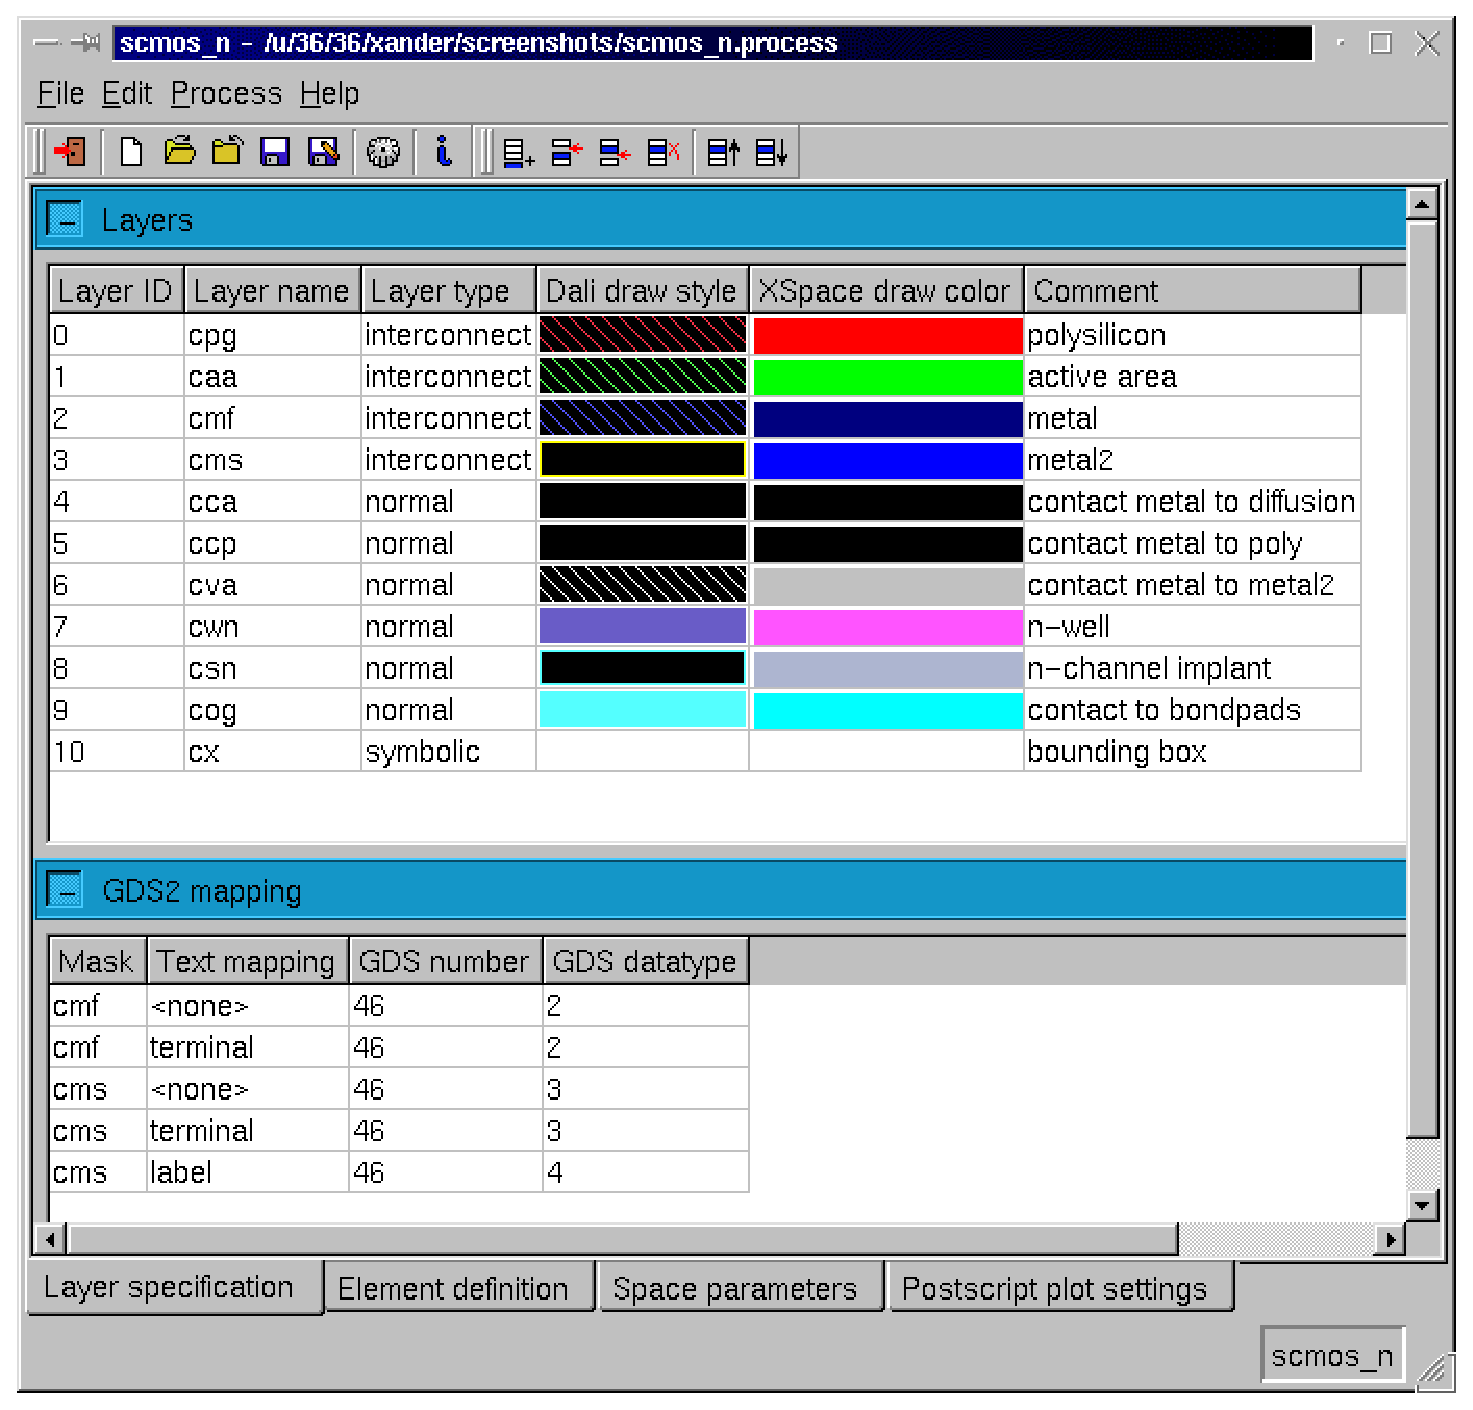
\includegraphics[width=7cm]{./figures/partition.eps}%mainwindow_layers.eps}
\caption{Partitioning and subpartitioning. The tabpages represent the first
level of partitioning. The sections (the blue horizontal bars) provide the
subpartitioning.}
\label{fig:design:tabpages}
\end{center} \end{figure}


These ``parts'' can still contain much data that must be entered. The element
definition file is good example of this. It would be better if we partition
each part even further. An effective user interface must thus be able to handle
partitions with sub-partitions.

\bigskip \noindent
The big question is now how we can achieve this. The first rough partitioning
that corresponds to the files can be implemented using ``tabpages''. Each
tabpage will correspond to a file or a general aspect of the process
description. The elements on the tabpage will describe the data that must be
entered.

As mentioned before, it would be profitable if we could further partition a
tabpage. Some files just will not fit on a tabpage. For this purpose, a custom
widget named the ``section'' widget was designed. It is described in detail in
Section \ref{sect:uidesign:section}. With this widget, a tabpage can be divided
into multiple sections, that can be shown either expanded or collapsed. A
collapsed section hides a part of its interface. This mechanism allows for a
much clearer arrangement of the user interface. Figure
\ref{fig:design:tabpages} shows the tabpages and sections in action.


%%%%%%%%%%%%%%%%%%%%%%%%%%%%%%%%%%%%%%%%%%%%%%%%%%%%%%%%%%%%%%%%%%%%%%%%%%%%%
\section{Design methodology and conventions}
Before each part of the design is discussed some remarks about the design
methodology and the used conventions are is place.

\bigskip \noindent
The \emph{Design Patterns} as described by Erich Gamma et al \cite{Gamma} are
used in the discussion of several parts of the design. These design patterns
provide a common vocabulary for computer program designers and therefore
references to these patterns will occur throughout the text.

\bigskip \noindent
Doxygen was used to generate the source code documentation. It is also capable
of generating so-called collaboration graphs, although the term collaboration
graph can be a bit misleading. The collaboration graphs generated by
\verb=doxygen= are a mix of what are called class diagrams and collaboration
diagrams in some well-known notations like Booch or UML.

In several places the collaboration graphs generated by
\verb=doxygen=\cite{doxygen} are used. Doxygen is a source code documentation
generator. The term

%%%%%%%%%%%%%%%%%%%%%%%%%%%%%%%%%%%%%%%%%%%%%%%%%%%%%%%%%%%%%%%%%%%%%%%%%%%%%
\section{The parser} \label{sect:design:parser}
To be able to read and interpret the configuration file, a parser has been
created. The parser consists of three parts (as shown in Figure
\ref{fig:design:parser}):
\begin{enumerate}
\item a lexical analyzer
\item a grammar parser
\item a class that provides methods for the parser to build the component tree
and the generators.
\end{enumerate}
The lexical analyzer scans the configuration file for keywords and other
special language elements like string delimiters and parentheses. The lexical
analyzer used is generated by \emph{flex}\footnote{flex is a lexical analyzer
based on and compatible with lex.}. Recognized keywords and elements are called
\emph{tokens}.

The lexical analyzer is used by the grammar parser. This grammar parser can
recognize and analyze a series of \emph{tokens}. It can then perform actions
related to the sequence of tokens it encountered. The grammar parser is
generated with \emph{bison}\footnote{bison is a parser based on and compatible
with the well-known grammar parser yacc.}. For more information about the
language used in the configuration file, please refer to \mbox{Chapter
\ref{chap:language}}.

\begin{figure} \begin{center}
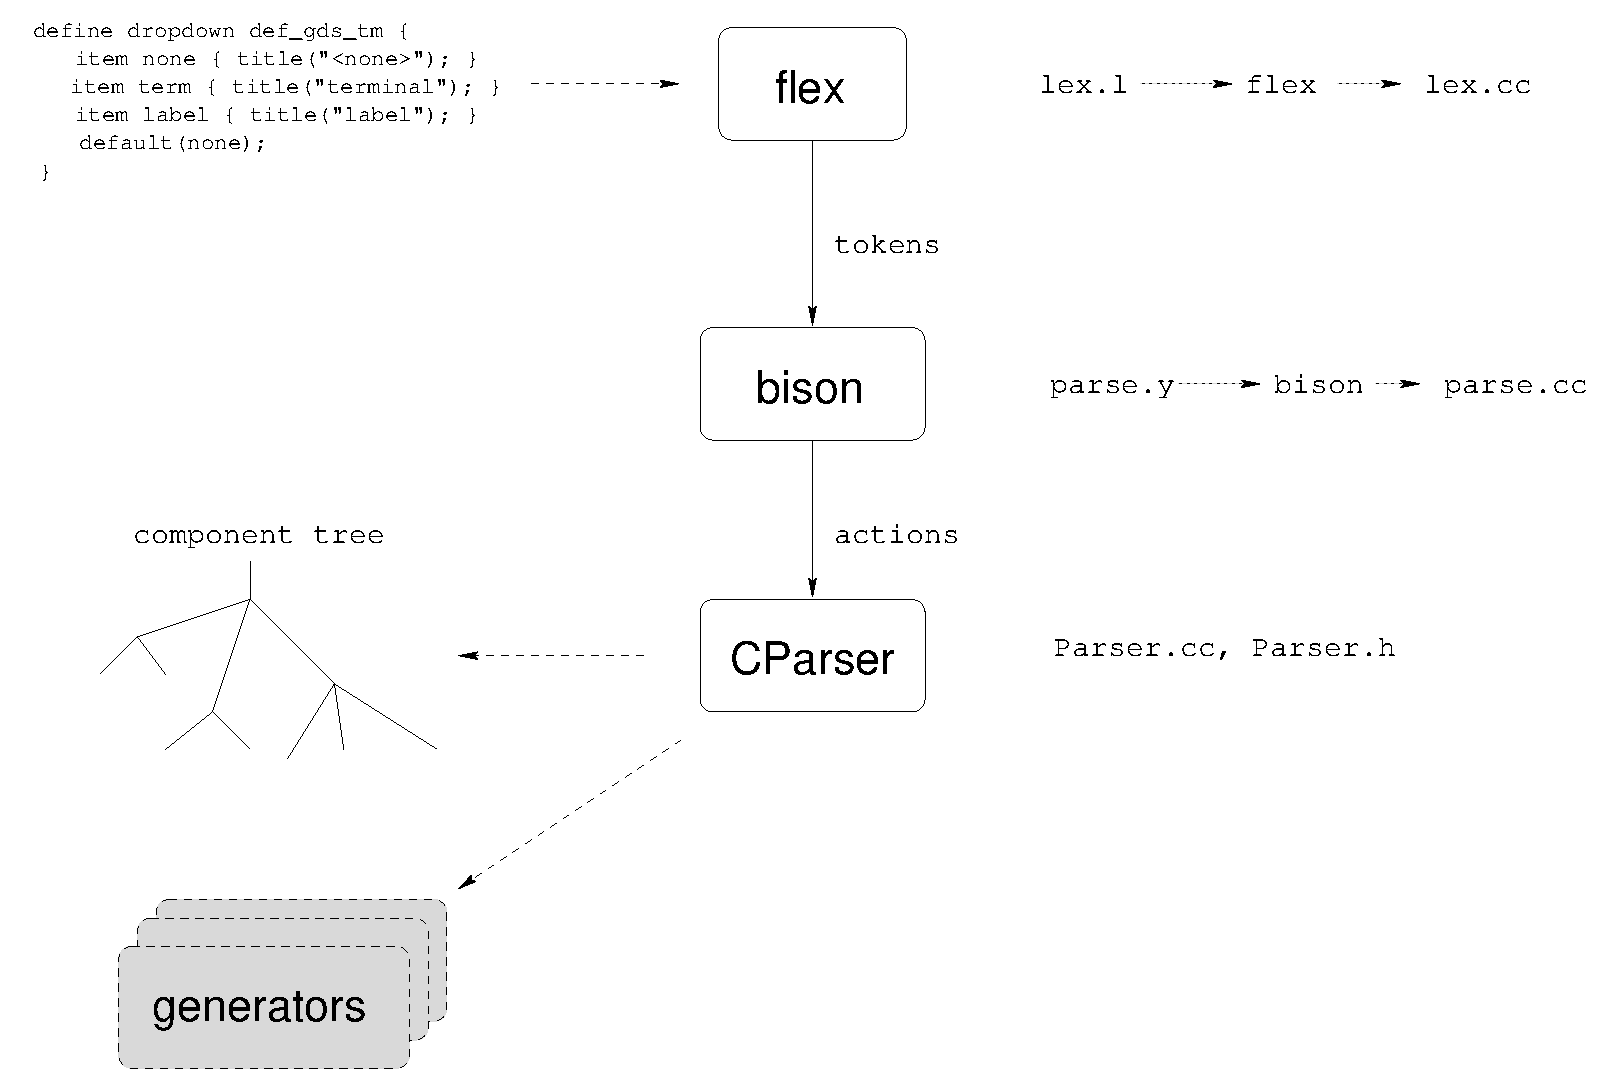
\includegraphics[width=12cm]{./figures/parser.eps}
\caption{The path from configuration file to component tree and generator data
structures. On the right side the files containing the implementation.}
\label{fig:design:parser}
\end{center} \end{figure}

The actions that the parser performs are the methods provided by the parser
class, \verb=CParser=. The \verb=CParser= class builds the component tree and
the generators, which are described in the following sections. The
\verb=CParser= class also extends the functionality of the parser generated by
bison:
\begin{itemize}
\item Disambiguation of identifiers specified in the configuration file. If
ambiguities arise, these are reported. \item The \verb=CParser= class also acts
as a \emph{builder}\footnote{A simplified version of the \emph{builder} pattern
described by Gamma et al \cite{Gamma} is used here.} for the component trees
and generators.
\item The \verb=CParser= class is implemented as a \emph{singleton}\footnote{The
\emph{singleton} pattern as described by Gamma et al \cite{Gamma}.}. This
ensures that only one instance of the parser will be created and that this
instance will be easily accessible.
\item Errors in the configuration file are reported in a dialog box in
stead of on the console. The line number of the line(s) containing the error(s)
are also reported.
\end{itemize}

%%%%%%%%%%%%%%%%%%%%%%%%%%%%%%%%%%%%%%%%%%%%%%%%%%%%%%%%%%%%%%%%%%%%%%%%%%%%%
\section{Components and the component tree} \label{sect:design:components}
The parser described in the previous section creates a tree, as is illustrated
in Figure \ref{fig:design:overview} and Figure \ref{fig:design:parser}. This
tree is called the component tree and consist of instances of the
\verb=CComponent= class.

In the following sections, the structure and abilities of the component tree
will be explained.

\subsection{Structure}
The tree is based on the \emph{composite} pattern, as described in Gamma et al
\cite{Gamma}. The difference between the composite pattern and the structure
used here is the lack of the ``leaf'' nodes. Only the ``composite'' nodes are
used in the component tree. The reasons for this are simple:
\begin{itemize}
\item The number of nodes in the component tree is relatively small. The
argument of efficient memory usage by using separate classes for leaves and
composite nodes is a weak one in this case.
\item The complexity decreases, thereby simplifying implementation.
\end{itemize}
Root components are tied together in the \verb=CComponentTree= class. The
collaboration graph for the \verb=CComponentTree= is shown in \mbox{Figure
\ref{fig:doxygen:CComponentTree_coll}}

\begin{figure}[ht]
\begin{center}
\includegraphics[height=2cm]{./figures/class_ccomponenttree_coll_graph.eps}
\caption{CComponentTree collaboration graph.}
\label{fig:doxygen:CComponentTree_coll}
\end{center}
\end{figure}
As can been seen in \mbox{Figure \ref{fig:doxygen:CComponentTree_coll}} the
\verb=CComponentTree= contains references to the \verb=CComponents= that are
root components. The \verb=CComponent= class contains references to
\verb=CComponents= that are either the parent component (\verb=m_parent=) or
child components (\verb=m_children=).

\subsection{CComponent and CComponentTree abilities}
\label{sect:design:component_abilities}
The \verb=CComponent= class provides the following functionality for its
clients:
\begin{itemize}
\item Name and context methods
\item Property support
\item Simple type support
\item Parent/child access
\end{itemize}

\bigskip \noindent
\textbf{Name and context methods} control access to the components name.
Components have names that function as an identifier. The names of the parent
components concatenated with dots form the ``context'' in which the identifier
lives. For example, if \verb=A= is a parent of \verb=B= and \verb=B= is the
parent of
\verb=C= then \verb=A.B= is the context of \verb=C= and \verb=A.B.C= is the
``full-context name'' of component \verb=C=.

Access to names and contexts is provided by the \verb=setName()=,
\verb=getName()= and \verb=getFullContextName()= methods.

\bigskip \noindent
\textbf{Property support} is something not provided by C++. C++ requires
explicit set and get methods for class members. Properties would be very useful
for the
\verb=CComponent= class. Many different types of components will be described
by the \verb=CComponent= class and properties would make this easier.
Inheritance is also an option, but the number of classes required would be too
large to implement in the given time.

Property support is therefore added to the \verb=CComponent= class by providing
methods like \verb=setProperty()= and \verb=getProperty()=. The properties are
stored in the STL\footnote{STL is the Standard Template Library, which is part
of the C++ standard. The STL provides containers, algorithms, strings, streams
and many other utility classes.} container \emph{map}. A property can have
\emph{multiple} values, because the values are stored as a vector of strings.
For more implementation specifics, please refer to the source code
documentation \cite{SPOCK}.

\bigskip \noindent
\textbf{Simple type support} must be present to be able to differentiate
between the component types. Type support is very crude, only methods like
\verb=setType()= and \verb=getType()= are implemented. There is currently no
support for type checking and type conversion.

\bigskip \noindent
\textbf{Parent/child access} and modification is also provided. The available
methods include:
\begin{itemize}
\item \verb=getParent()= retrieves a pointer to the parent component
\item \verb=add()= adds a child to this component
\item \verb=removeChild()= removes a child from the list of children
\item \verb=getChild()= can retrieve a pointer to a child component
\item \verb=numChildren()= and \verb=childPos()= provide array--like access to
the children.
\end{itemize}
Some of these methods have multiple implementations accepting different
arguments, increasing the flexibility of this much--used class.

\subsection{Component tree creation}
A prototype tree is created by the \verb=CParser= class described in
\mbox{Section \ref{sect:design:parser}}. The prototype tree is copied for every
process that is created with ``File $\rightarrow$ new'' or loaded into the
application. The reasons for this will be explained further in \mbox{Section
\ref{sect:design:uibuilder}}, where the user interface builder is described.

\subsection{Iterating through the component tree}
Iterating through the tree is necessary for building the user interface,
searching components, printing debug information about the components, etc.
Walking through the tree is such a common action that the interface should be
open to extension.

The \emph{visitor} pattern is applied to make the interface flexible. The
visitor pattern allows us to easily apply an operation to the component tree.
Some of the advantages of using the visitor pattern:
\begin{itemize}
\item The \verb=CComponent= class is not polluted by methods and attributes related to
a certain operation on the entire tree. This related behaviour is placed in the
visitor class instead.
\item The visitor pattern makes it easy to define new operations on the tree.
Adding a new visitor is all that is required.
\item Visitors can also accumulate state as they visit each component in the
component tree. This is done for example in the FindComponentVisitor, which
counts the number of hits.
\end{itemize}
The visitor pattern is described in Gamma et al. \cite{Gamma}.

\subsubsection*{Available visitors}
The available and by \verb=CComponentTree= accepted visitors are listed in
Table \ref{tab:design:visitors}. The implementation of the
\verb=CFindComponentVisitor=, \verb=CFindPropertyVisitor= and
\verb=CDumpComponentTreeVisitor= is straightforward and the interested reader
is referred to the source code documentation.
\begin{table}
\caption{Visitors and their purpose}
\label{tab:design:visitors}
\begin{tabular}{l|p{6cm}}
\hline
 \textsf{Visitor} & \textsf{Description} \\
\hline  %\hline
    \verb=CFindComponentVisitor= & Retrieves all components with a given name. \\
%\hline
    \verb=CFindPropertyVisitor=  & Retrieves all components that have the specified
    property. The value specified is compared with the value of the property
    considered. The comparison criterion can be specified as either equal or
    unequal. This could be extended with larger/smaller criteria in future
    versions. \\
%\hline
    \verb=CDumpComponentTreeVisitor= & This visitor prints the (indented)
    tree to the console. This visitor is provided for debugging purposes. \\
%\hline
    \verb=CGUIBuilderVisitor= & The GUI build process is described in detail in
    \mbox{Section \ref{sect:design:uibuilder}}.\\
    \verb=CSerializerVisitor= & Provides means to load or save the information
    entered by the user and stored in this tree. This is discussed in Section \ref{sect:design:serialization}\\
\hline
\end{tabular}
\end{table}

\verb=CSerializerVisitor= and \verb=CGUIBuilderVisitor= are not so
straightforward. The \verb=CGUIBuilderVisitor= class is described in detail in
Section \ref{sect:design:uibuilder}. The \linebreak \verb=CSerializerVisitor=
and serialization\footnote{Serialization is the term used for the process of
saving and loading application data.} in general is discussed in Section
\ref{sect:design:serialization}.


%%%%%%%%%%%%%%%%%%%%%%%%%%%%%%%%%%%%%%%%%%%%%%%%%%%%%%%%%%%%%%%%%%%%%%%%%%%%%
\section{The user interface builder}\label{sect:design:uibuilder}
So, after parsing the configuration file the component tree is created and
ready to be processed further. The user interface builder creates the actual
widgets (the basic user interface elements) from the component tree by visiting
the tree with the \verb=CGUIBuilderVisitor=.

The creation of the user interface is thus a two step process:
\begin{enumerate}
\item The component tree with the structure of the user interface is created
from the configuration file.
\item The \verb=CGUIBuilderVisitor= visits the component tree and creates a
\verb=CGUITree= object that contains the created widgets and provides methods
to access them.
\end{enumerate}

One might wonder why the component tree does not contain the widgets and why
the \verb=CGUIBuilderVisitor= is needed. After all, all the information related
to the user interface is already ``in there''. The reasons behind this are
actually quite straightforward:

\begin{itemize}
\item The hierarchy Qt uses for its widgets is different from the one used by
the component tree. The Qt tree is very fine-grained compared with the
component tree and incorporates layout information for the widgets.
\item If we were to include the creation and management of the Qt widgets in
the component tree, the \verb=CComponent= class would get ``bloated''. The
\verb=CComponent= class would serve two different purposes (\verb=CComponent=
parent/child management and Qt widget management), which is usually bad
software engineering.
\end{itemize}

\subsection{The CGUIBuilderVisitor}
The \verb=CGUIBuilderVisitor= first determines the type of the component being
visited. It then calls the method needed to build that type of component. These
(private) methods are listed in Table \ref{tab:design:CGUIBuilderVisitor}.

The widgets created are mapped to the components whenever this is desired. This
mapping allows us to access the value a user enters in the widget using the
\verb=CGUITree=. The mapping is described in detail in the next section.

\begin{table} \begin{center}
\caption{CGUIBuilderVisitor build methods.}
\label{tab:design:CGUIBuilderVisitor}
\begin{tabular}{l|p{6cm}}
\hline
 \textsf{Method}          & \textsf{Description}                                                                                                                     \\
\hline
 \verb=buildTabPage()=           & Creates a tabpage. A tabpage usually contains only a scrollframe.                                                                 \\
 \verb=buildScrollFrame()=       & Creates a scrollframe. A scrollframe can contain multiple widgets. If they do not fit inside the frame, scrollbars are displayed. \\
 \verb=buildSection()=           & Creates a section. A section can contain multiple widgets, including nested sections.                                             \\
 \verb=buildParamList()=         & Creates an empty parameter list.                                                                                                  \\
 \verb=buildSpreadSheet()=       & Creates an empty spreadsheet.                                                                                                     \\
 \verb=buildSpreadSheetColumn()= & Adds a column to the current spreadsheet.                                                                                         \\
 \verb=buildComboBox()=          & Creates combobox and dropdown widgets.                                                                                            \\
 \verb=buildLineEdit()=          & Creates a line edit.                                                                                                              \\
\hline
\end{tabular} \end{center} \end{table}


\subsection{The CGUITree}
The \verb=CGUITree= created by the \verb=CGUIBuilderVisitor= provides a mapping
between a component tree and the Qt widgets related to that tree. The methods
provided reflect this.

\paragraph{The mapping methods} allow creating a mapping and retrieval of
values from the mapping. To create a mapping between a component and a widget
\verb=makeMapping()= can be used. To retrieve either a component given a widget
or a widget given a component, \verb=getComponent()= or \verb=getWidget()= can
be used. As a special case, \verb=getTabPages()= retrieves all the tabpages in
the gui tree.

\paragraph{Value methods} are also implemented. These consist of get/set
methods for normal components and get/set methods for spreadsheets. The
spreadsheet methods take the column component as an extra argument. The methods
are named \verb=getValues()=, \verb=setValues()=, \verb=getSpreadSheetValues()=
and \linebreak \verb=setSpreadSheetValues()=.

\paragraph{Other methods} provided include methods for data connections, which
will be discussed in Section \ref{sect:design:dataconnections}.
\verb=findComponent()= is implemented as a convenience function. It calls the
associated component tree's \verb=findComponent()= method. Also implemented are
some slot\footnote{slots are part of Qt's signal/slot mechanism which allow
sending and receiving signals to and from objects.} methods needed by the
spreadsheets. More about this in Section \ref{sect:uidesign:spreadsheet} where
the spreadsheet widget is explained.

\bigskip \noindent
A partial collaboration diagram showing the classes discussed is presented in
Figure \ref{fig:design:guibuilder_partial}.

\begin{figure} \begin{center}
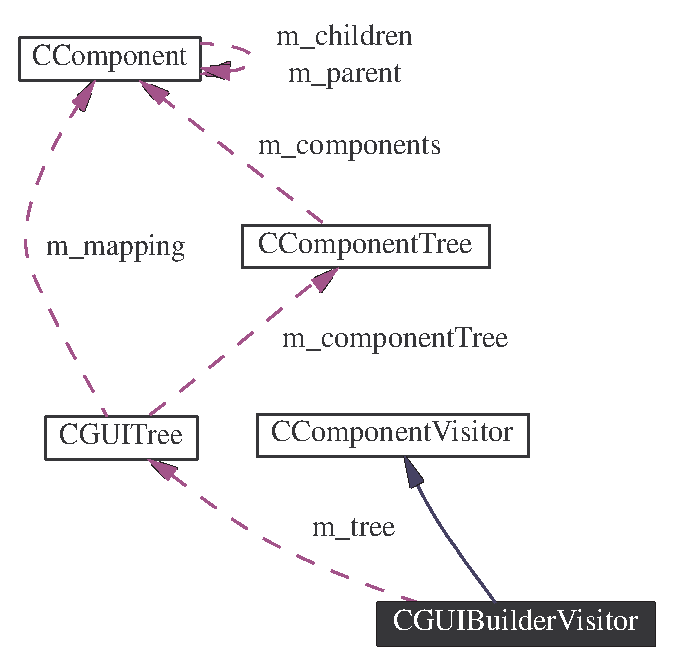
\includegraphics[width=7cm]{./figures/guibuilder_partial.eps}
\caption{Partial collaboration diagram for class CGUIBuilderVisitor}
\label{fig:design:guibuilder_partial}
\end{center} \end{figure}

%%%%%%%%%%%%%%%%%%%%%%%%%%%%%%%%%%%%%%%%%%%%%%%%%%%%%%%%%%%%%%%%%%%%%%%%%%%%%
\section{Data connections} \label{sect:design:dataconnections}
An important feature that partly determines the success of the chosen approach
is the ability to use the data entered by the user in other fields. For
example, in some part of the user interface the user must specify which layers
exist in the application. In some other part, the user must map a layer to a
GDS2 number. It would be convenient if the user could choose from the defined
layers. This not only reduces the chance of (typing) errors, it also makes the
user interface more comfortable to work with.

\bigskip \noindent
This dynamic behaviour is implemented by the data connection classes. A data
connection consists of one or more data sources, a single data target and a
data connection object that is responsible for the actual synchronization of
values between the sources and the target. This is depicted in Figure
\ref{fig:design:dataconnections}.

\begin{figure} \begin{center}
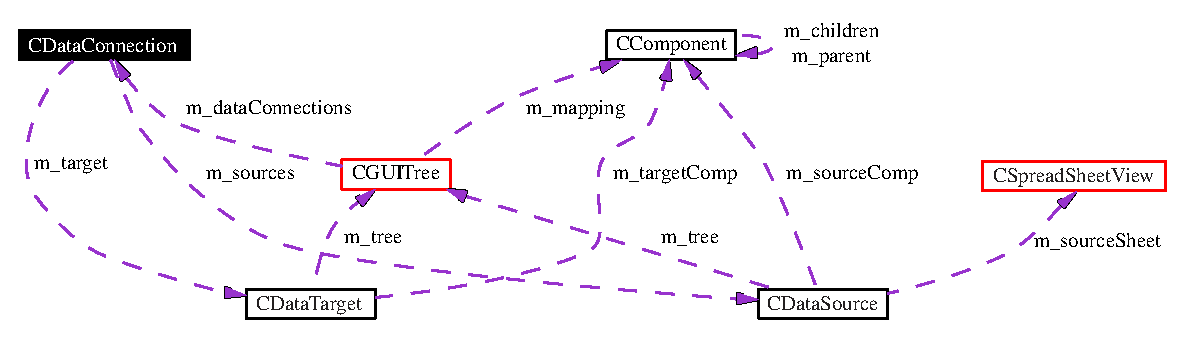
\includegraphics[width=12cm]{./figures/class_cdataconnection_coll_graph.eps}
\caption{Data connection collaboration diagram.}
\label{fig:design:dataconnections}
\end{center} \end{figure}

The implementation relies heavily upon the Qt signal/slot mechanism. This
mechanism implements the \emph{observer} pattern \cite{Gamma}. The dynamics of
this construction are expressed in Figure \ref{fig:design:datadynamics}. The
\verb=CDataSource= object ``detects'' a change in the value it watches. It then
signals the \verb=CDataConnection= object that the target needs updating. The
\verb=onSynchronize()= method then calls \verb=updateValues()= for the correct
\verb=CDataTarget= object.

%% figure goes here.
\begin{figure} \begin{center}
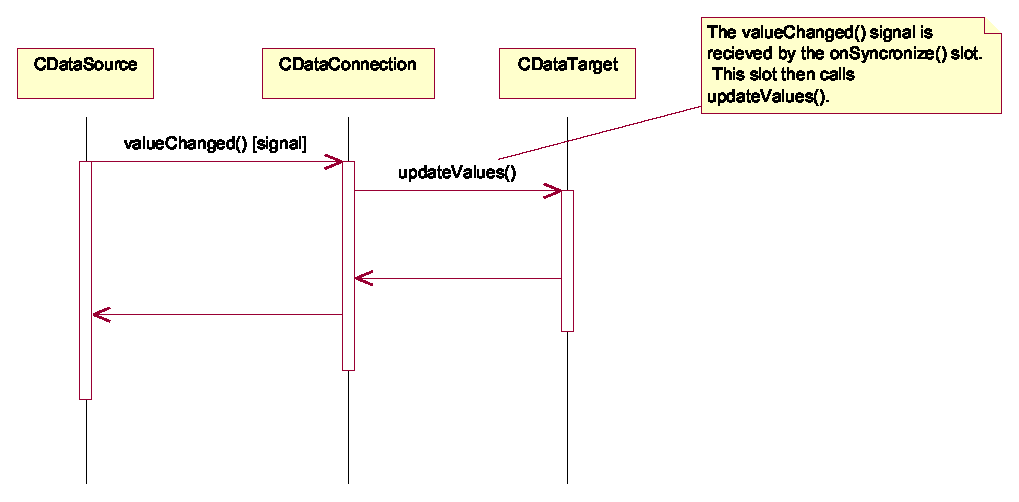
\includegraphics[width=10cm]{./figures/dataconnection_dynamics.eps}
\caption{Example of Qt's signal/slot mechanism.}
\label{fig:design:datadynamics}
\end{center} \end{figure}

Currently, there is only one type of data source supported. This is the column
of a (custom) spreadsheet widget. The constructor checks if the source
component specified is a column in a spreadsheet. The \verb=getValues()= member
is tailored to retrieve the values from a spreadsheet column.

Support for different types of data sources can easily be added. The methods
involved are declared virtual. This means a new \verb=CDataSource= derived
class supporting the new type of source can easily be added.

The \verb=CDataTarget= class already has some derived classes. They are listed
(and explained) in Table \ref{tab:design:datatargets}.

\begin{table} \begin{center}
\caption{Possible data targets.}
\label{tab:design:datatargets}
\begin{tabular}{l|l}
\hline
 \textsf{Derived class name}     & \textsf{Description}                          \\
\hline
 \verb=CColumnDataTarget=        & The data target is a column in a spreadsheet. \\
 \verb=CComboDataTarget=         & The data target is a combobox like component  \\
 \verb=CConditionListDataTarget= & The data target is a condition list.          \\
\hline
\end{tabular}
\end{center} \end{table}

%%%%%%%%%%%%%%%%%%%%%%%%%%%%%%%%%%%%%%%%%%%%%%%%%%%%%%%%%%%%%%%%%%%%%%%%%%%%%
\section{Technology file generation} \label{sect:design:filegeneration}
The file generation architecture strongly resembles the architecture used to
build the user interface. Figure \ref{fig:design:filegeneration} presents this
architecture. If we compare this process with the one that creates a user
interface we can see a lot of similarities. Both start from a definition given
in the configuration file. This definition is then parsed and a component tree
is created.

\begin{figure} \begin{center}
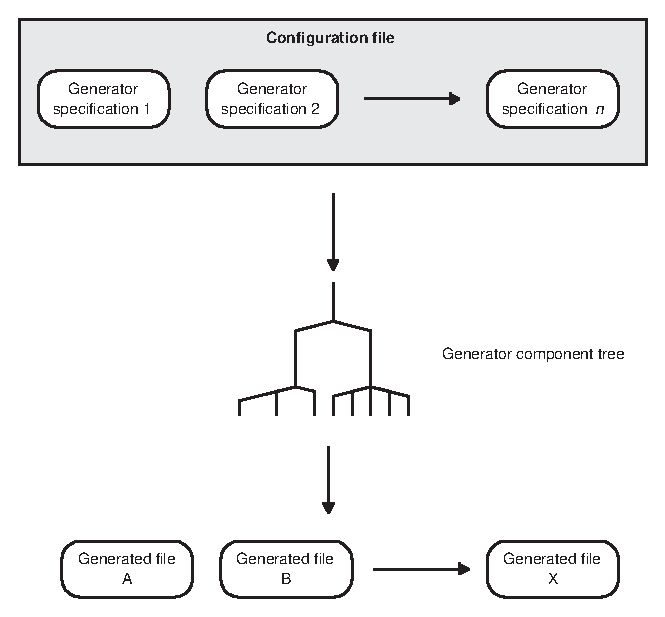
\includegraphics[width=8cm]{./figures/file_generation.eps}
\caption{Overview of the file generation process.}
\label{fig:design:filegeneration}
\end{center} \end{figure}

The datastructures used for the file generation process are discussed next,
followed by a description of the generation process itself.

\subsection{File generation datastructures}
As mentioned before, the format specifications defined in the configuration
file are parsed and put into an expression tree. Like the component tree, this
tree structure uses the \verb=CComponent= class for its nodes. However, the
tree interpretation is different. The nodes of the component tree represent a
part of a hierarchy, while the nodes of the expression tree represent an action
that should be performed (possibly involving the nodes' children).

For the file generator, the nodes in the tree can all be evaluated to plain
text. The tree structure represents the more elaborate language constructs,
like the \verb=foreach= loops and \verb=if= constructions. These constructs can
affect the eventual result. More information on these language constructions
can be found in Chapter \ref{chap:language}.

\bigskip \noindent
The root components of the tree represent the generators. The class used for
the root components is the \verb=CGeneratorComp= component. This is a
\verb=CComponent= derived class. The added functionality lies in the support of
value maps.

A value map allows the ``translation'' of dropdown item text to the text that
should be generated instead. This mapping applies to all instances of the
dropdown in that tree. In a future version of the application this behaviour
could be extended to include other types of substitution as well.

\bigskip \noindent
The generators are collected in the \verb=CGenerators= class. Currently, the
interface only provides methods for access to the generators. They are listed
in Table \ref{tab:design:CGenerators}.

\begin{table} \begin{center}
\caption{Methods provided by the CGenerators class}
\label{tab:design:CGenerators}
\begin{tabular}{l|l}
\hline
 \textsf{Method}          & \textsf{Description}  \\
\hline
 \verb=addGeneratorComp()=       & Adds a generator to the list of generators.\\
 \verb=numGenerators()=          & Returns the number of generators. \\
 \verb=getGenerator()=           & Retrieves the desired generator.\\
\hline
\end{tabular} \end{center} \end{table}

The \verb=CGenerators= class could be extended with additional methods if the
need for them arises.

\subsection{The generation process}
Generating the files starts with the user bringing up the generation dialog
box. As can be seen in Figure \ref{fig:design:generatedialog} each file can be
generated separately. The result can be saved into a specified directory or
into the SPACE process tree directly (if the user has the required rights).
This is explained in detail in Section \ref{sect:design:integration}. Before
the files are actually written to disk they can be inspected and edited if the
user checks the ``Edit and inspect results'' option.

\begin{figure}[!bh] \begin{center}
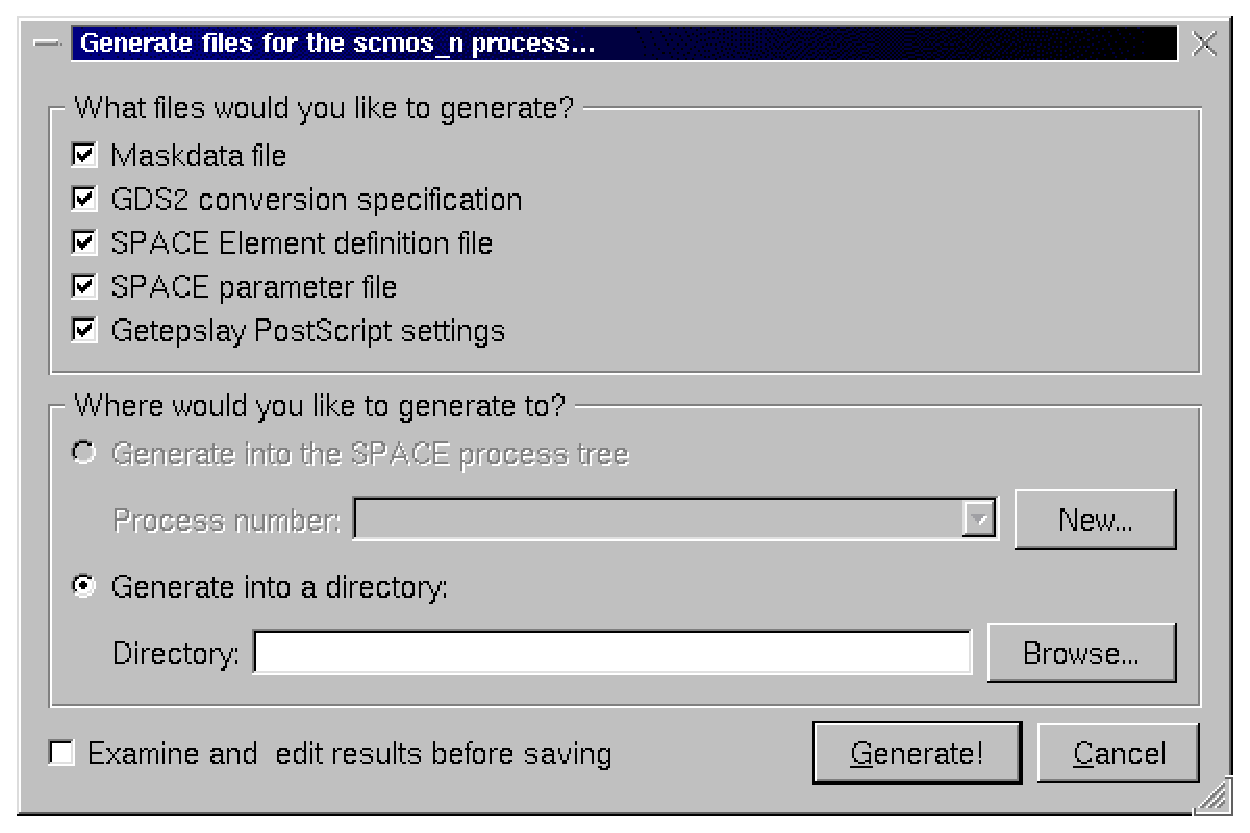
\includegraphics[width=7cm]{./figures/generate.eps}
\caption{The technology file generation dialog box.}
\label{fig:design:generatedialog}
\end{center} \end{figure}
After all the required information is gathered, the \verb=generateFile()=
method from the \verb=CProcess= class is called for each file that must be
generated. This method evaluates the file's generator tree to the file's
contents. The evaluation of the nodes is done by some private helper methods
included in the \verb=CProcess= class. They include the generation of literals,
identifiers, numbers, binary operators like addition and subtraction, \verb=if=
constructions and \verb=foreach= constructions. It is also possible to request
some information from the application. These include process name and
description and time and date of generation.

To allow nested \verb=foreach= loops a dedicated class was written that
contains the state of an iteration. The class is named \verb=CIteratedState=
and instances of this class are put into a stack by the \verb=CProcess= class
as necessary.

\subsection{Integration with the SPACE process tree} \label{sect:design:integration}
As was mentioned in the previous section, it is also possible to generate the
result directly into the SPACE process tree.

SPACE keeps the technology files for each process in a separate directory. The
name of the directory is also the name of the process. The process directories
all reside inside a directory that also contains the \verb=processlist= file.
This file contains a list of the processes mapped to a certain number. Changing
the number of a process is potentially dangerous and should be avoided.

To generate a process into the SPACE process tree, an update of the
\verb=processlist= file is required. The user must either select the correct
number or enter a new number for the process to be generated. To aid the user,
the comments after each mapping are read and displayed together with the
numbers and names of the processes in the \verb=processlist= file.

\bigskip \noindent
If the user proceeds with the generation process, the \verb=processlist= file
is rewritten to disk. The entry of the generated process is added or replaced
(depending on the users' choice for the process number). The comment after the
new entry will contain the process description.

%%%%%%%%%%%%%%%%%%%%%%%%%%%%%%%%%%%%%%%%%%%%%%%%%%%%%%%%%%%%%%%%%%%%%%%%%%%%%
\section{Serialization} \label{sect:design:serialization}
With serialization we mean storing or retrieving the data describing a process
to or from disk. The flexibility of the application makes this quite difficult
however, as will be explained in the following sections.

\subsection{Serialization method}
The data that must be serialized is entered by the user in the user interface.
The user interface is generated from the configuration file. This means that
the method used to serialize the data must somehow include this information.

The obvious solution is to bundle the data and the user interface description
present in the configuration file. However, this introduces a problem that is
unacceptable. The whole idea of the chosen approach was to introduce
flexibility. If we bundle the data and the user interface description, changes
made to the configuration file are useless. The old configuration file that was
bundled with the data will be used instead, thus effectively eliminating the
introduced flexibility.

\bigskip \noindent
To prevent the problem described above, the data is stored as key-value pairs.
The key is the full context name of the component associated with the data. The
value is the actual value in the user interface. This ensures that every value
can be restored, even if additions have been made to the configuration file.

Unfortunately, this approach has it defects as well. Defects that can largely
be overcome though.

\subsection{Compatibility issues}
The proposed method of serializing the data works as long as the full context
names of the components are still the same as in a newer configuration file.
Since the full context name also contains information about how the user
interface is arranged, moving parts of the user interface can be disastrous.

For example, in version 1 of the configuration file we have the component
\verb=A.B.C.D=. In version 2 we would like to have \verb=C.D= somewhere else.
Let us assume we want to move it to \verb=A.E=, resulting in \verb=A.E.C.D=. It
is clear that the old version 1 files cannot be read by the version 2
configuration file, although no real changes in the data have occurred.

To solve this problem, a disambiguation method has been implemented. If the
full context name cannot be resolved, context is added to the components name
until a single match is found. Continuing the previous example, this would mean
the search would start with \verb=D=. If \verb=D= is not unique, \verb=C= is
added to the context, resulting in \verb=C.D=. In this case, \verb=A.E.C.D= is
the unique component found.

\bigskip \noindent
Renaming components between versions is another issue. Renaming can be solved
by adding methods that can translate old version names to new version names.
This means editing source. As a result, renaming components is an action that
causes a major version change. This is acceptable, since renaming is mostly
done because of the esthetics of the configuration file.

Adding and removing components is no problem. Adding a component means the
component will be set to the default since it is not present in the old
version. Removing a component means that the component cannot be found if an
old version file is loaded. In this case, nothing happens.

\subsection{Implementation}
Because values are stored by their component name, a \emph{visitor} can be used
here. The visitor is called \verb=CSerializerVisitor=. The most important
methods are listed in Table \ref{tab:design:CSerializerVisitor}.

\begin{table} \begin{center}
\caption{Important methods provided by the CSerializerVisitor class}
\label{tab:design:CSerializerVisitor}
\begin{tabular}{l|p{6cm}}
\hline
 \textsf{Method}                  & \textsf{Description}                                                                                                  \\
\hline
 \textsf{readConversion()}        & While reading a file, converts an identifier-value pair from an old version to a new version. Currently does nothing. \\
 \textsf{writeConversion()}       & While writing a file, converts an identifier-value pair from this version to an old version. Currently does nothing.  \\
 \textsf{guessCorrectComponent()} & Tries to resolve relocated components.                                                                                \\
 \textsf{doFileInit()}            & Reads or writes the file header. The header contains the process name and description.                                \\
\hline
\end{tabular}
\end{center} \end{table}

\section{The application}
A screenshot of the application in action is shown in Figure
\ref{fig:design:app_screenshot}.

\begin{figure} \begin{center}
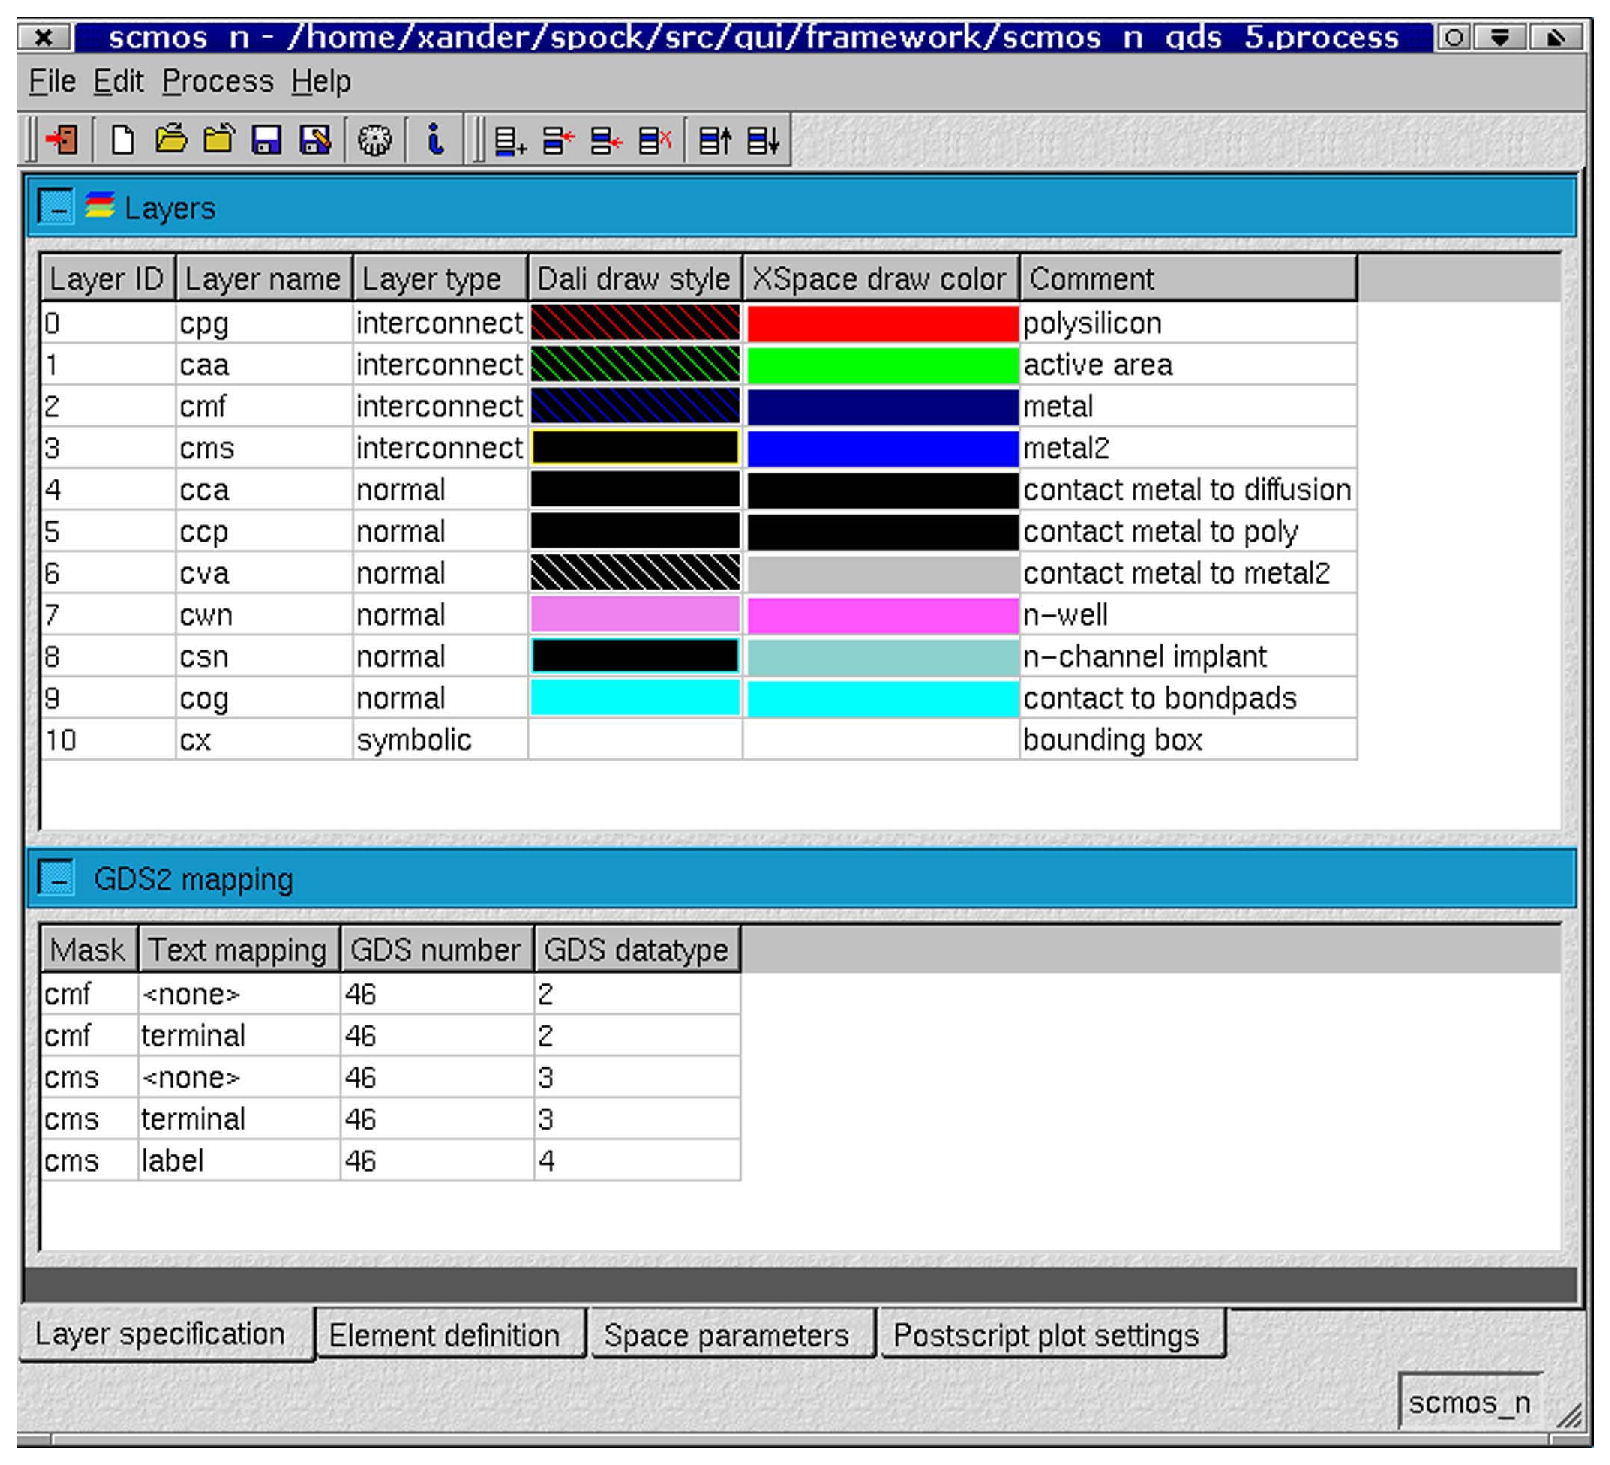
\includegraphics[width=8cm]{./figures/app_action.eps}
\caption{The application in action.}
\label{fig:design:app_screenshot}
\end{center} \end{figure}

As was already mentioned in Section \ref{sect:design:integration}, the
technology files can be generated directly into the SPACE process tree. This is
just one aspect of the relationship between the SPACE and the application.

\subsubsection*{Place of the configuration file}
The configuration file should be present either in the directory the
application was started from or in
\texttt{\$ICDPATH$\backslash$lib$\backslash$spock}. The filename should be
\verb=spock.uis=. If the file is not found in either location the application
will exit. \texttt{\$ICDPATH} is an environment variable that should point to
the SPACE installation location.

\subsubsection*{Existing technology files}
Unfortunately, existing technology files cannot be read by the application.
Only the processes entered in the application and saved in the applications'
own file format can be read.

%%%%%%%%%%%%%%%%%%%%%%%%%%%%%%%%%%%%%%%%%%%%%%%%%%%%%%%%%%%%%%%%%%%%%%%%%%%%%
\section{Recommendations for future features} \label{sect:design:future}
Although the application is already quite complete, there is always room for
improvement. Some recommendations were already mentioned somewhere in this
chapter. These recommendations are included in the list below.

\begin{itemize}
\item \textbf{Components and the component tree} \\ Better type support. Type
checking and type conversion routines could be implemented.
\item \textbf{Data connections} \\ Support for more types of data sources and
targets could be implemented.
\item \textbf{Generator value maps} \\ The value substitution method used by
the generators only supports substitution of dropdown and combobox values
defined in the configuration file. This mechanism could be extended to include
arbitrary substitution of values.
\item \textbf{Framework enhancements} \\ The framework user interface could be
extended to include cut, copy and paste operations. An undo/redo feature would
also be a useful addition.
\end{itemize}
\noindent Recommendations for the configuration file language can be found in
\mbox{Chapter \ref{chap:language}.}

%\begin{itemize}
%\item Components and the component tree
%    \begin{itemize}
%    \item Better type support. Type checking and type conversion routines
%    could be implemented.
%    \end{itemize}
%\item Data connections
%    \begin{itemize}
%    \item Support for more types of data sources and targets could be
%    implemented.
%    \end{itemize}
%
%\end{itemize}

%%%%%%%%%%%%%%%%%%%%%%%%%%%%%%%%%%%%%%%%%%%%%%%%%%%%%%%%%%%%%%%%%%%%%%%%%%%%%
\section{Graphical overview} \label{sect:design:conclusions}
In this last section a graphical overview of the completed and implemented
design is presented.

\bigskip \noindent
Figure \ref{fig:design:complete_overview} contains a complete high-level
overview of the design. Clearly visible are the similarities between the GUI
creation part of the application and the file generating part of the
application.

\begin{figure}[b!] \begin{center}
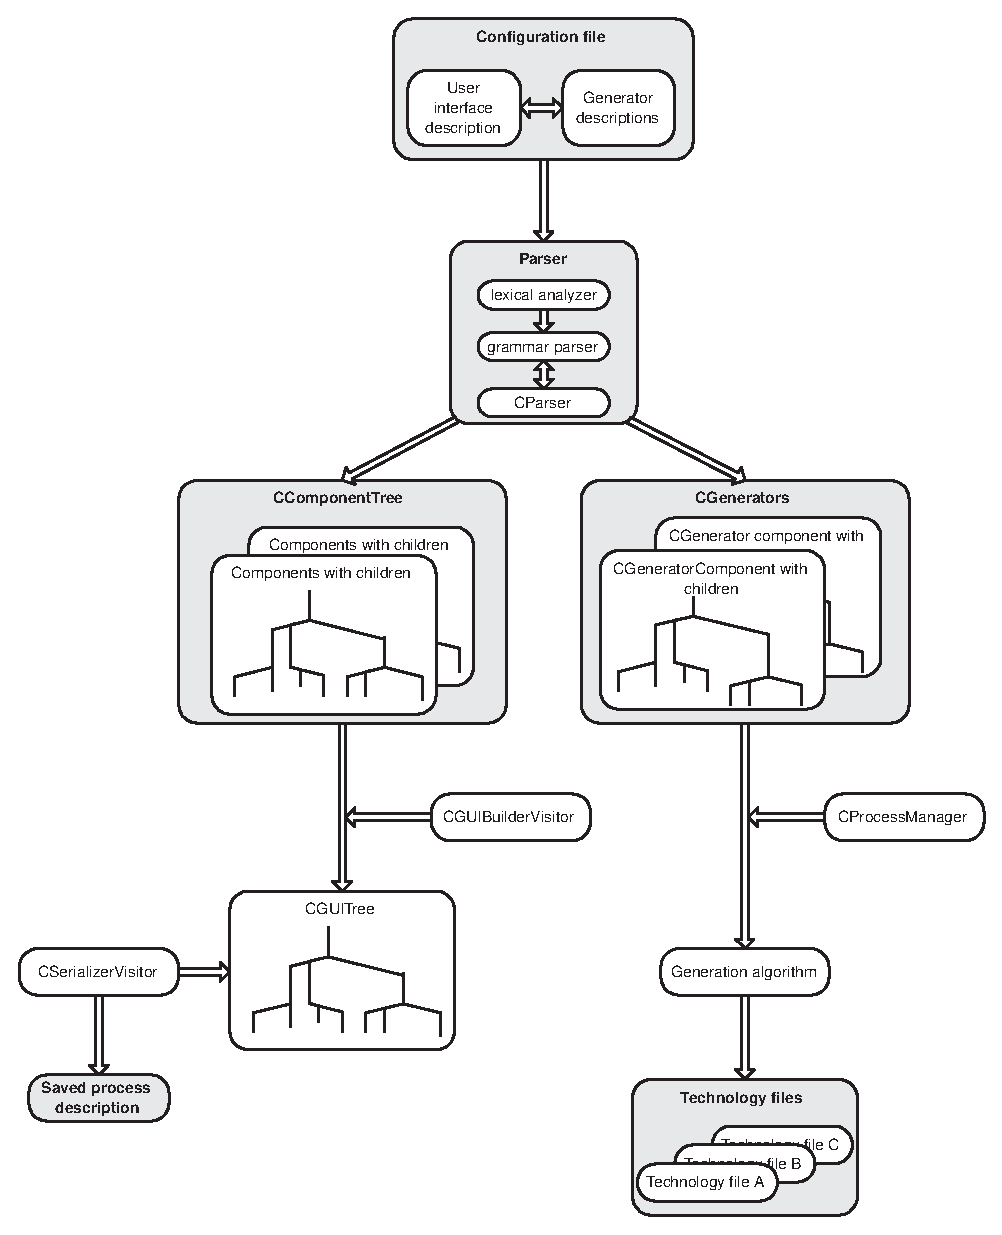
\includegraphics[height=10cm]{./figures/complete_overview.eps}
\caption{Complete architecture overview}
\label{fig:design:complete_overview}
\end{center} \end{figure}

\bigskip \noindent
Figure \ref{fig:design:complete_class} contains the class diagram as reverse
engineered by Rational Rose (a graphical design tool). Associations due to
connected signals and slots are not shown here, since Rational Rose cannot
handle these special Qt constructs.

The central role of the \verb=CGUITree= and \verb=CComponent= tree class is
quite clear.

\begin{figure} \begin{center}
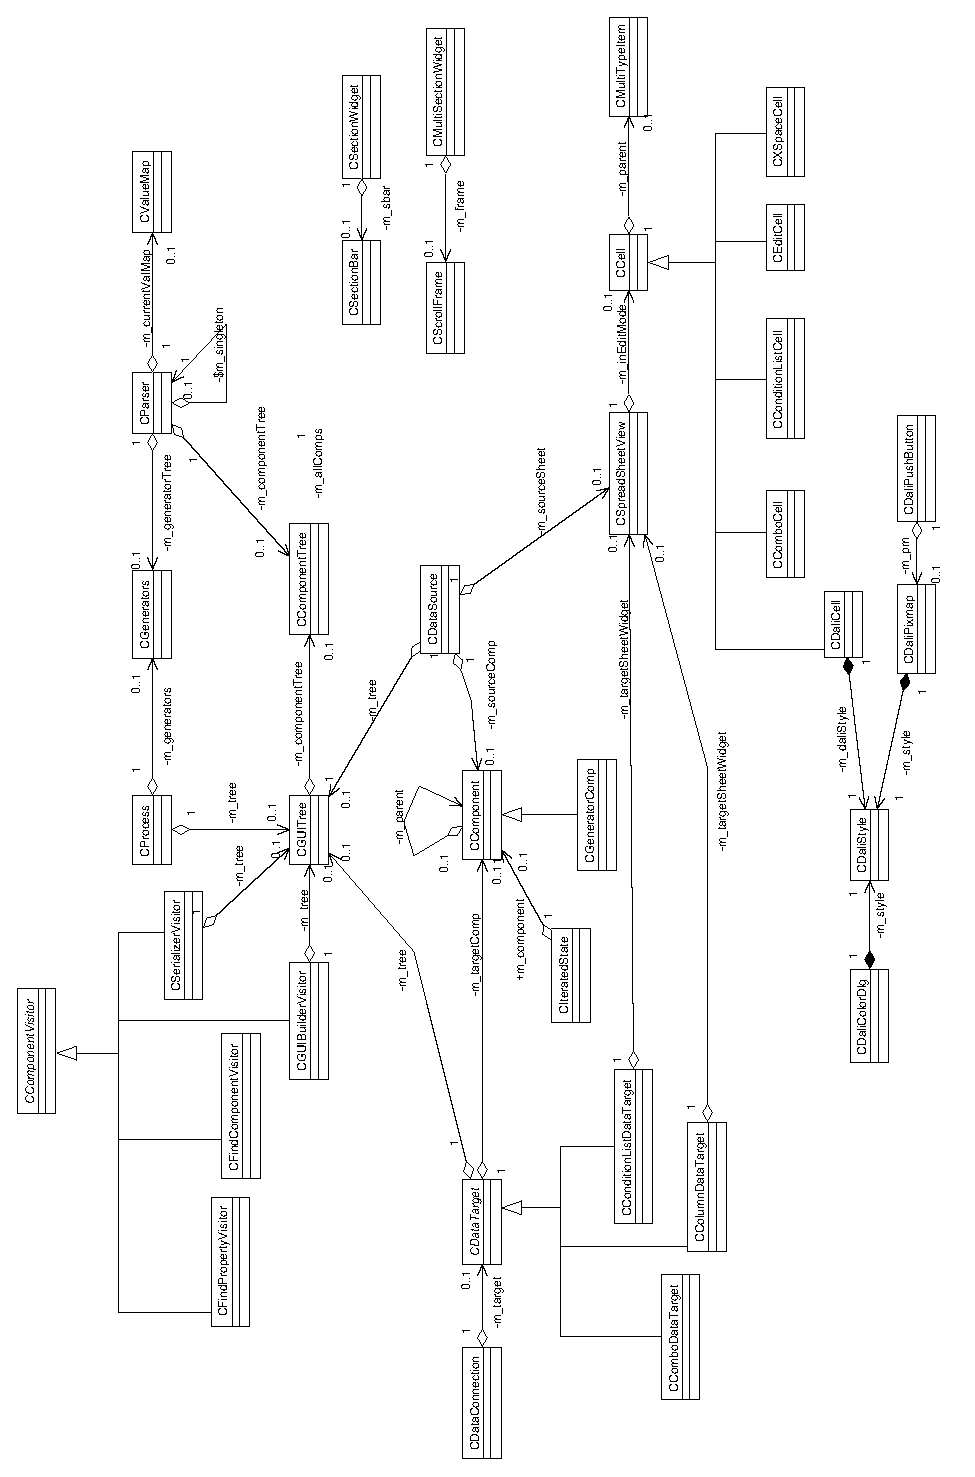
\includegraphics[width=12cm]{./figures/complete_class_diagram.eps}
\caption{Class diagram as reverse engineered by Rational Rose 2000}
\label{fig:design:complete_class}
\end{center} \end{figure}

% uidesign.tex

\chapter{User interface elements} \label{chap:uidesign}
C++ does not have a default user interface library. Therefore, the user
interface architecture presented in Section \ref{sect:design:ui_architecture}
needs to be implemented with a special toolkit. This toolkit will supply a set
basic elements that can be extended with custom, specialized elements.

\bigskip \noindent
The main goal of this chapter is to present the user interface elements the
application uses. These are the user interface elements provided by the chosen
toolkit as well as some custom elements.

\bigskip \noindent
The choice for a specific toolkit is made in Section
\ref{sect:uidesign:toolkit}. After that decision has been made, the user
interface elements supported by that toolkit will be described briefly. The
custom user interface elements will then be presented in Section
\ref{sect:uidesign:custom}.

%%%%%%%%%%%%%%%%%%%%%%%%%%%%%%%%%%%%%%%%%%%%%%%%%%%%%%%%%%%%%%%%%%%%%%%%%%%%%
\section{Choosing a user interface toolkit} \label{sect:uidesign:toolkit}
There are several widget toolkits available for all flavors of unix operating
systems. The most popular toolkits that interface directly with C/C++ are
listed below:
\begin{itemize}
\item Motif or Lesstiff
\item The Athena widget library
\item GTK+
\item Qt
\end{itemize}

\bigskip \noindent
\textbf{Motif (or Lesstiff)} is well known. Motif provides a rich set of user
interface elements and is quite powerful. The main disadvantage of Motif is the
old C-style function based interface.


\bigskip \noindent
\textbf{The Athena widget library} is also function based. The Athena widget
set is very easy to learn but (as a consequence perhaps) not as rich as for
example Motif.

\bigskip \noindent
\textbf{GTK+} is used in GNOME. It is a very complete toolkit. Contrary to
Motif and Athena, this toolkit is object oriented. It is also a portable
toolkit, although it has many dependencies that can make compilation difficult.

\bigskip \noindent
\textbf{Qt} is the toolkit on which the KDE window manager is based. Qt
\cite{Qt} is also very complete and object oriented. It was designed with
portability in mind and is available for all Unix platforms as well as for
Windows. There is even a version for embedded devices. It also provides an
extension to C++ with the signal/slot mechanism.

\bigskip \noindent
The choice seems to be between Qt and GTK+. Qt was chosen because of its
portability and the signal/slot mechanism.

%%%%%%%%%%%%%%%%%%%%%%%%%%%%%%%%%%%%%%%%%%%%%%%%%%%%%%%%%%%%%%%%%%%%%%%%%%%%%
\section{Qt native user interface elements}
Qt's complete list of user interface elements is too large to describe here.
The elements that will be described next are the ones that are supported by the
configuration file language as well as those that are used for the custom
widgets. Readers that are already familiar with these widgets can skip to
Section \ref{sect:uidesign:custom}.

\subsection{Labels and edits}
Labels and editable widgets are heavily used. They are implemented by the
\verb=QLabel= and \verb=QLineEdit= classes.

A label is a frame containing text. This text cannot be changed by the user.
Contrary to this, the edit widget \emph{can} be changed by the user. The main
use for this type of widget is to retrieve numbers or text from the user.

Figure \ref{fig:uidesign:label_edit} shows these two widgets in action.

\begin{figure}[ht] \begin{center}
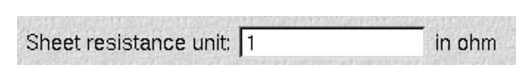
\includegraphics[height=5mm]{./figures/label_edit.eps}
\caption{Two label widgets and one edit widget.}
\label{fig:uidesign:label_edit}
\end{center} \end{figure}

\subsection{Dropdowns and comboboxes}
Dropdowns can be used if the user can choose a value from a list of known
values. A combobox should be used if it must also be possible for the user to
type in a value not found in the list.

For example, suppose the user must enter a month name. In this case, a dropdown
should be used containing the twelve moths of the year. Now suppose the user
must enter a word he would like to search for in a document. It is common
practice to also let the user choose from the last few search terms. In this
case the combobox contains the last few search terms but it is still possible
to enter a new search term.

\bigskip \noindent
Figure \ref{fig:uidesign:combobox} shows a combobox. The widgets are
implemented by the \verb=QComboBox= class. Dropdown behaviour can be achieved
by making the \verb=QComboBox= read only.

\begin{figure}[ht] \begin{center}
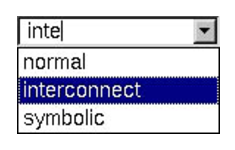
\includegraphics[height=15mm]{./figures/combobox.eps}
\caption{A combobox widget.}
\label{fig:uidesign:combobox}
\end{center} \end{figure}

\subsection{Listview}
The listview widget is often used to display files and their properties. A
screenshot of listview is depicted in Figure \ref{fig:uidesign:listview}.
\begin{figure}[ht] \begin{center}
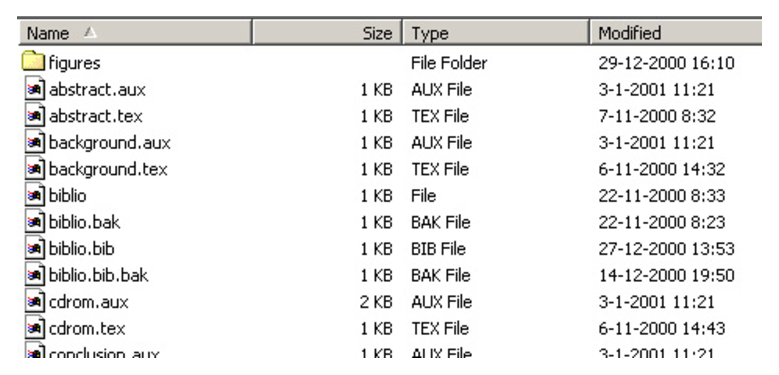
\includegraphics[height=3cm]{./figures/listview.eps}
\caption{A listview widget used to display files.}
\label{fig:uidesign:listview}
\end{center} \end{figure}
Listviews usually have multiple columns. Clicking a row selects the entire row
and editing is limited to the first column, if editing is allowed at all.

\subsection{The color select dialog box}
Color selection is also directly provided by Qt. The \verb=QColorDialog= class
implements a color selection dialog that can be called and used with one line
of code. A screenshot is shown in Figure \ref{fig:uidesign:colordialog}.

\begin{figure}[hb] \begin{center}
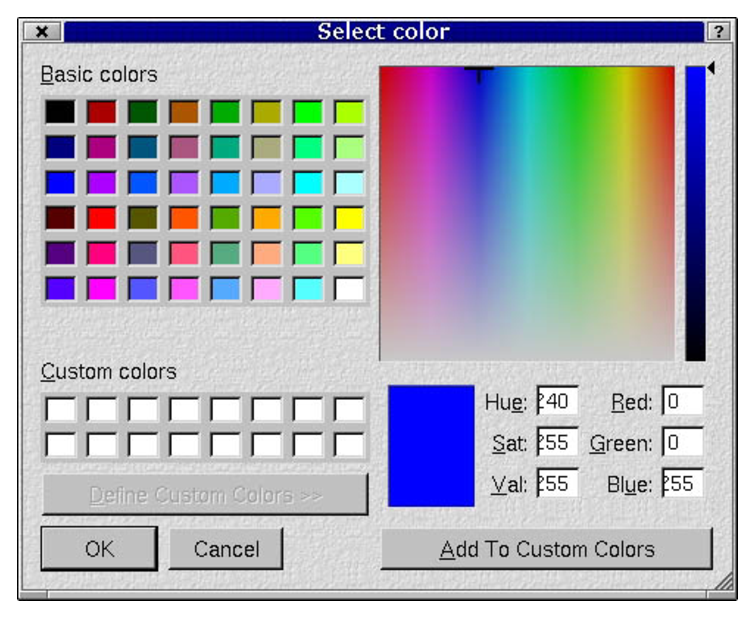
\includegraphics[height=5cm]{./figures/color.eps}
\caption{The Qt color selection dialog box.}
\label{fig:uidesign:colordialog}
\end{center} \end{figure}

%%%%%%%%%%%%%%%%%%%%%%%%%%%%%%%%%%%%%%%%%%%%%%%%%%%%%%%%%%%%%%%%%%%%%%%%%%%%%
\section{Custom user interface elements} \label{sect:uidesign:custom}
Not a single toolkit provides the specialized widgets a programmer always seems
to need. The reason for this is simple: toolkits are designed to be general.
However, extending the toolkit should be easy and with Qt it really is.

The widgets created can be split into two categories:
\begin{enumerate}
\item Organizational widgets.\\ These widgets alter the presentation and layout of the widgets
they contain. These are the scrollframe and the section widget.
\item Data entry widgets.\\ These widgets provide a new way to enter data.
These are the spreadsheet widget, the conditionlist dialog and the dali
colorpicker dialog.
\end{enumerate}

\subsection{The scrollframe widget}
The scrollframe widget is used when a part of the user interface becomes to
large to display on the screen. If this happens, the scrollframe widget will
show horizontal and/or vertical scrollbars that can be used to ``scroll'' the
user interface to show the hidden parts.

The best place for them is inside the tabpages. If the widgets will not fit in
the space the tabpage has available, the scrollbars will be shown.

\subsection{The section widget} \label{sect:uidesign:section}
The section widget is a widget that can show or hide it's contents on the users
request. It is especially useful if used in combination with other section
widgets. Section widgets can be nested if desired. It is recommended to make
them part of a scrollframe, as expanding all the widgets will require a lot of
space.

\begin{figure}[ht] \begin{center}
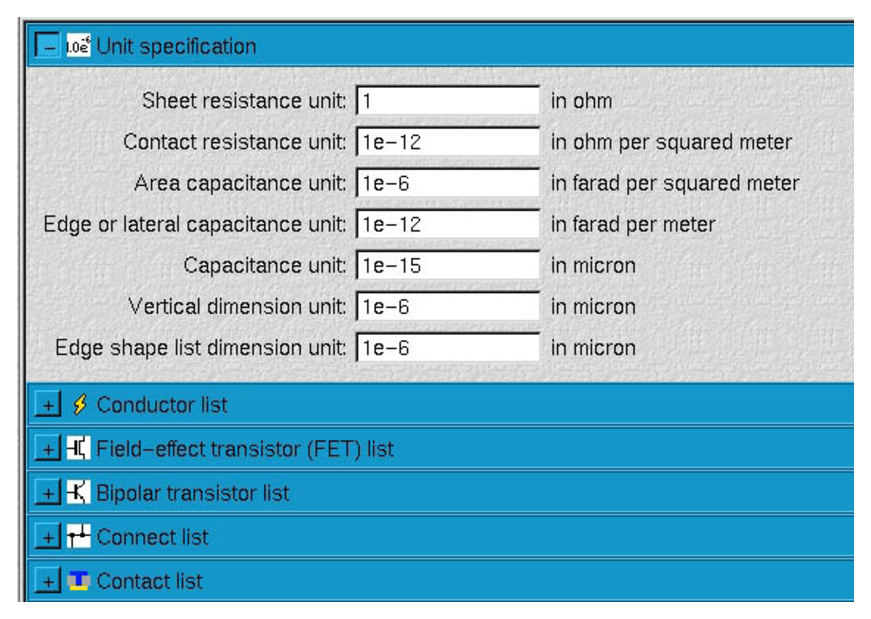
\includegraphics[height=6cm]{./figures/section.eps}
\caption{A few section widgets.}
\label{fig:uidesign:section}
\end{center} \end{figure}

The section widget is demonstrated in Figure \ref{fig:uidesign:section}. The
section widget is a blue bar with a button and a label. It is also possible to
add an icon between the button and the label. If a section is expanded the
button is shown pressed and it will contain a -- sign, indicating it can be
collapsed. If a section is collapsed the button is shown depressed and it will
contain a + sign, indicating it can be expanded.

The section widget has been created to add an extra level of partitioning to
the user interface. This has been discussed in detail in Section
\ref{sect:design:generatedui}.

\subsection{The spreadsheetview widget} \label{sect:uidesign:spreadsheet}
The spreadsheetview widget is a hybrid of a spreadsheet and a listview,
extended with behaviour to make the widget more generally applicable.

\bigskip \noindent
The spreadsheetview visually resembles the listview. However, the default
listview behaviour is not adequate for our purposes. The main deficiencies are
listed below:
\begin{itemize}
\item Editing a cell can only be done with a simple in-place text edit widget.
\item Only the cells in the first column can be edited.
\item Only cells containing text are allowed.
\item The selection and focus behaviour is row oriented and not cell oriented.
\end{itemize}
What we would like to see is a listview in which each cell can be edited. The
way in which a cell can be edited should not be restricted to entering text. It
should be possible to use comboboxes or even dialog boxes to enter a value in a
cell. For example, to specify a layer's color, a cell that can display the
current selected color is necessary. Editing this cell should somehow allow the
user to pick any of the available colors.

The best way to implement this in a flexible way is by using an abstract
\verb=CCell= class. Deriving from this class allows the implementation of
specialized behaviour. There are already five \verb=CCell= derived classes
implementing special cell behaviour. They are listed below:

\begin{itemize}
\item \verb=CEditCell= implements a regular text cell that can be edited with
an in-place line edit.
\item \verb=CComboCell= implements a combobox and dropdown cell. The normal
display is plain text. The edit mode brings up an in-place dropdown or
combobox.
\item \verb=CColorCell= shows a color. The edit mode brings up the default Qt
color select dialog box.
\item \verb=CDaliCell= shows colors and fills as used in dali. The edit mode
brings up the dali colorpicker dialog (which will be described later in this
chapter).
\item \verb=CConditionListCell= shows a conditionlist in the format used in the
SPACE element definition files. The edit mode brings up the conditionlist
editor (which will be described later in this chapter).
\end{itemize}

The spreadsheetview widget is shown in Figure
\ref{fig:uidesign:spreadsheetview}.

\begin{figure}[ht] \begin{center}
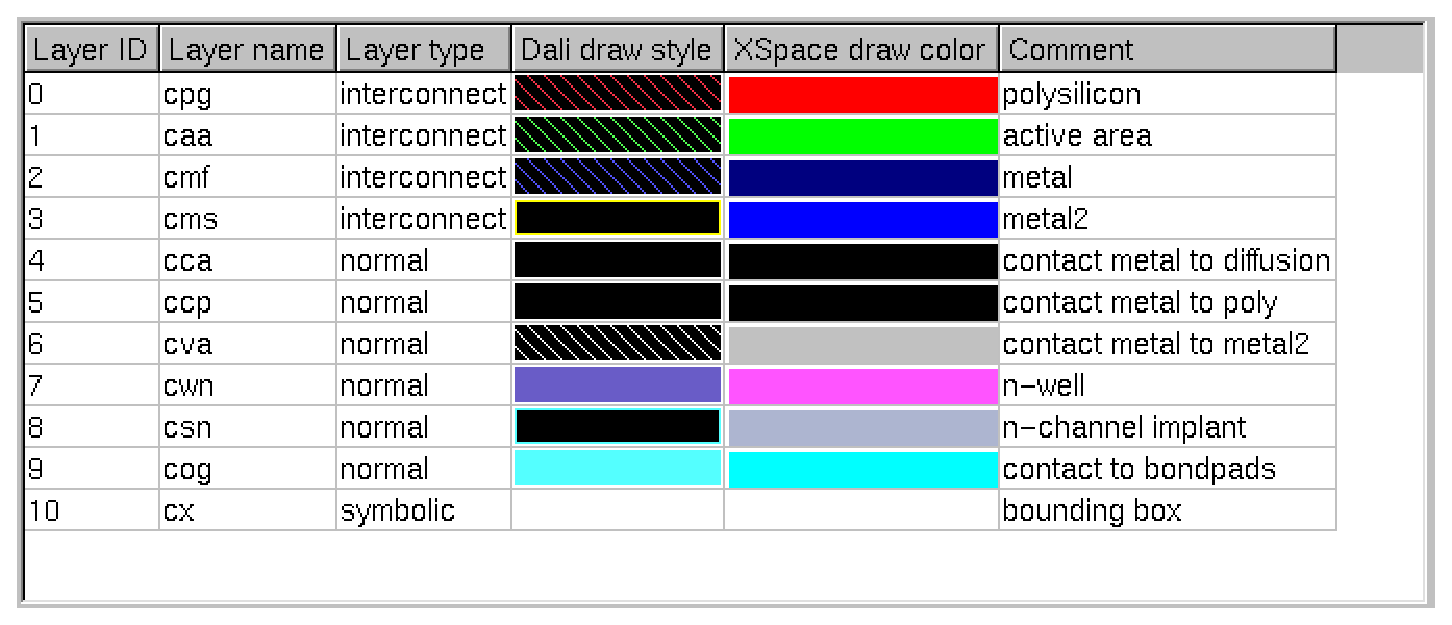
\includegraphics[width=8cm]{./figures/ex_spreadsheet.eps}
\caption{The spreadsheetview widget.}
\label{fig:uidesign:spreadsheetview}
\end{center} \end{figure}


\paragraph{Implementation\\ }
\noindent The spreadsheetview widget is implemented in the
\verb=CSpreadSheetView= class. This class is derived from the Qt
\verb=QListView= class. Also used in the implementation is the custom
\verb=CMultiTypeItem= class which is derived from the \verb=QListViewItem=
class. Finally, the \verb=CCell= class specifies the interface for the derived
classes and provides some basic functionality. The relationship between the
classes is shown in Figure \ref{fig:uidesign:spreadsheet_coll}.
\begin{figure} \begin{center}
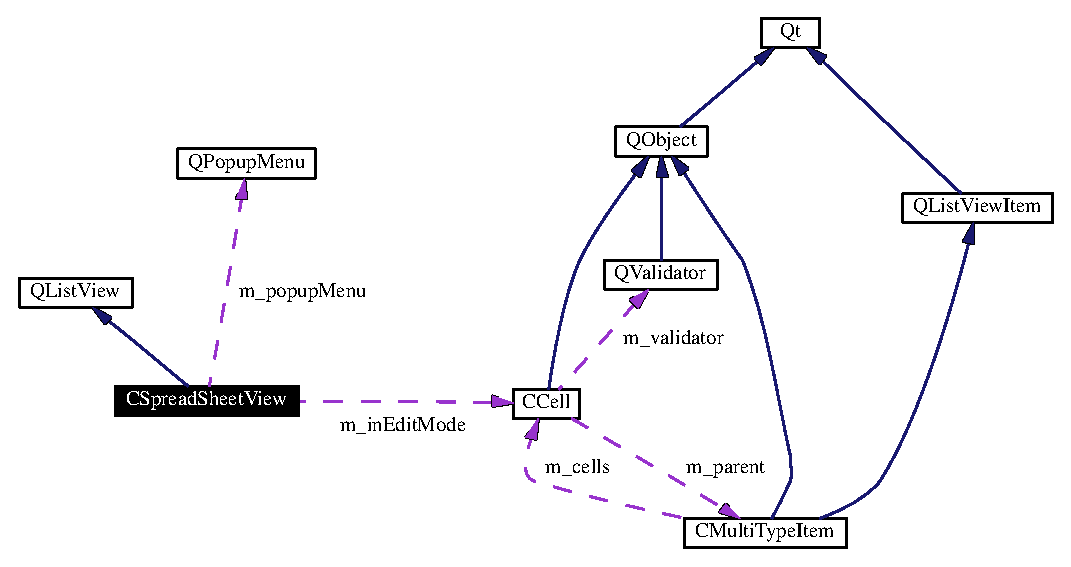
\includegraphics[width=10cm]{./figures/class_cspreadsheetview_coll_graph.eps}
\caption{CSpreadSheetView collaboration diagram.}
\label{fig:uidesign:spreadsheet_coll}
\end{center} \end{figure}

The collaboration diagram clearly shows that a \verb=CSpreadSheetView= is a
specialization of the \verb=QListView= class. The \verb=CMultiTypeItem= class
is a specialization of the \verb=QListViewItem= class and represents a row in
the spreadsheetview. The \verb=CMultiTypeItem= itself contains \verb=CCell=
objects, representing the columns in that row.

Figure \ref{fig:uidesign:spreadsheet_class} shows the class diagram. A
\verb=CSpreadSheetView= class contains rows, implemented by the
\verb=CMultiTypeItem= class. Each row consist of a number of \verb=CCell=
derived objects.

\begin{figure} \begin{center}
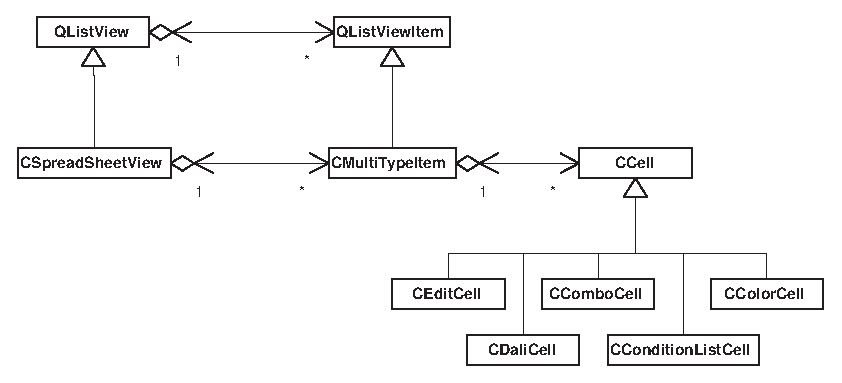
\includegraphics[width=10cm]{./figures/spreadsheet_class.eps}
\caption{CSpreadSheetView class diagram.}
\label{fig:uidesign:spreadsheet_class}
\end{center} \end{figure}


\bigskip \noindent
After the creation of a \verb=CSpreadSheetView= object, columns can be added
using the \verb=addColumn()= method. Rows can be added using the
\verb=addNewRow()= method. The creation of the \verb=CCell= objects is left to
the client. If a cell object needs to be created the \verb=CSpreadSheetView=
objects emits a \verb=pleaseCreateCell()= signal. The signal communicates the
\verb=CMultiTypeItem= (the row) and the column that needs a \verb=CCell=
(derived) object. If the \verb=CCell= object is not created after the signal
(either because the signal was not connected to a slot or the slot could not
create a object) a default \verb=CCell= will be created by the
\verb=CSpreadSheetView= itself.

This mechanism allows the client to provide its own \verb=CCell= derived
objects at any column/row combination

\bigskip \noindent
Starting and ending the edit mode of a cell is handled by the
\verb=CSpreadSheetView= class, calling the correct \verb=CCell= object methods
as needed. The latest version of Qt now includes a spreadsheet widget (which
was absent during the development of the \verb=CSpreadSheetView= widget). It
uses the same mechanism of cell abstraction and delayed creation. It also uses
start/end edit methods. Perhaps a future version of the \verb=CSpreadSheetView=
widget should be based on this new Qt widget instead of on the \verb=QListView=
widget.

\subsection{The condition list dialog} \label{sect:uidesign:conditionlist}
Condition lists are used often in the SPACE element definition files. A
condition list specifies how the presence of a particular element depends on
the presence or absence of the different masks \cite{SpaceMan}. Basically, it
is a boolean combination of mask names. A space means the AND operation should
be applied. A \verb=|= character corresponds to an OR operation and an
exclamation mark (!) in front of a mask name is a NOT. Additionally, in the
cases where adjacent tiles have a meaning, the -- and = characters specify one
or the other side of a tile. For more information please refer to the SPACE
User's Manual \cite{SpaceMan}.

\begin{figure} \begin{center}
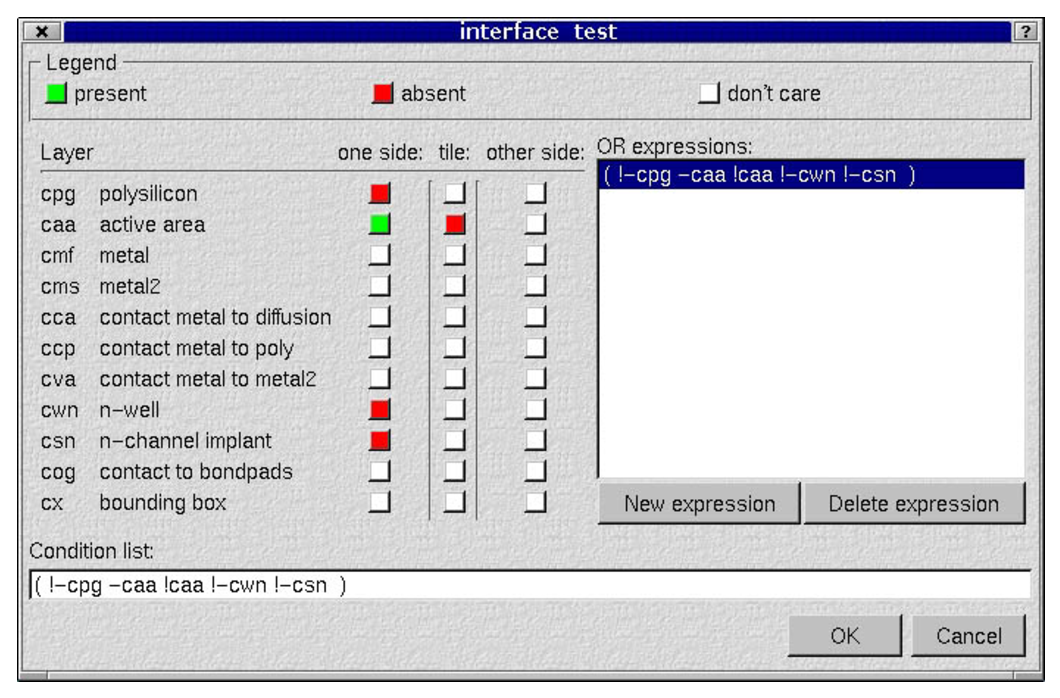
\includegraphics[width=9cm]{./figures/conditionlist.eps}
\caption{The conditionlist editor dialog box.}
\label{fig:uidesign:conditionlist}
\end{center} \end{figure}

\bigskip \noindent
The condition list editor is shown in Figure \ref{fig:uidesign:conditionlist}.
The condition list can be entered manually or by using the buttons and the
listbox. The layer names and descriptions are obtained using the data
connection mechanism described in Section \ref{sect:design:dataconnections}.
The special data target \verb=CConditionListDataTarget= has been implemented
for this to work. This allows to specify arbitrary sources for the layer names
and descriptions in the configuration file.

The listbox on the right side of the dialog box contains the OR expressions.
Each line in the listbox is OR-ed together to form the complete condition list.
Selecting an expression in this listbox will cause the buttons on the left side
to reflect the selected expression. Changing the button states will immediately
update the selected line in the listbox, as well as the line representing the
complete condition list.

\bigskip \noindent
The condition list editor supports two modes. In the default mode, only the
tile of interest is displayed. No neighboring tiles can be selected as present
or absent. In the extended mode, neighboring tiles are displayed as ``one
side'' and ``other side'' and can be selected as normal. The desired mode can
be specified in the configuration file.

\subsection{The dali colorpicker dialog}
The dali colorpicker dialog box lets the user select a color and fill style as
used in dali, the layout editor. Since dali understands only a limited set of
colors and fill patterns, the default Qt color dialog box and fill patterns
could not be used.

The colorpicker presents the user with a dialog box as shown in Figure
\ref{fig:uidesign:dalicolorpicker}. The dialog box consists of an array of
buttons. All the combinations of available colors with available patterns are
present. Clicking a button selects the color and fill represented by the
button.

\begin{figure}[hb] \begin{center}
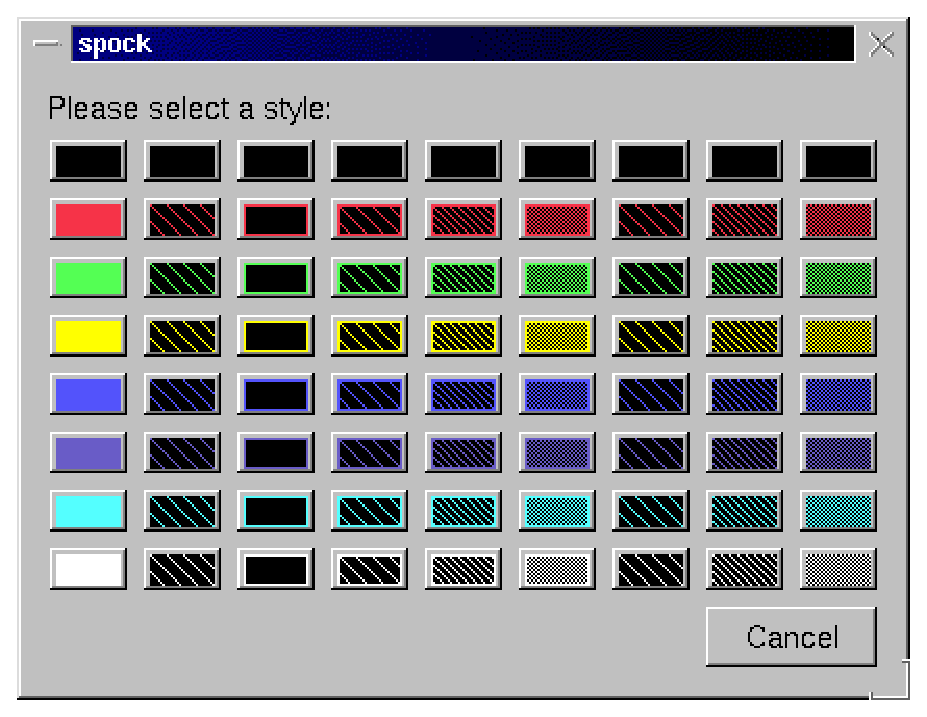
\includegraphics[width=6cm]{./figures/dalicolor.eps}
\caption{The dali colorpicker dialog box.}
\label{fig:uidesign:dalicolorpicker}
\end{center} \end{figure}

% language.tex

\chapter{The configuration file language} \label{chap:language}
The configuration file language was designed to be a flexible and easy to use (and
learn) language that can be used to specify a user interface, file generators
and the relationship between these two.

\bigskip \noindent
The main goal of this chapter is to present and explain the language and its
features.

\bigskip \noindent
First of all, some of the more general constructions used in the language are
presented and explained in Section \ref{sect:language:structure}. Because the
configuration file describes two different phenomena (user interface
specification and technology file format specification), a certain division of
the file is to be expected. Language constructions related to the user
interface are presented in Section \ref{sect:language:uiref}. Generator
constructions are described in Section \ref{sect:language:generatorref}.

%%%%%%%%%%%%%%%%%%%%%%%%%%%%%%%%%%%%%%%%%%%%%%%%%%%%%%%%%%%%%%%%%%%%%%%%%%%%%
%%%%%%%%%%%%\section{Language features} \label{sect:language:features}

%%\bigskip \noindent
%%The configuration file will contain the information that will eventually build
%%the component tree and the generators. This means that the language should
%%support some way of structuring. The elements that need to be structured are
%%the components (the nodes in the component tree) and the nodes of the generator
%%trees that will evaluate to plain text.
%%
%%Because of this subtle difference a difference in these two parts is to be
%%expected. The main structure of the file will be discussed next, followed by
%%these two parts, the user interface reference and the generator reference.

%%%%%%%%%%%%%%%%%%%%%%%%%%%%%%%%%%%%%%%%%%%%%%%%%%%%%%%%%%%%%%%%%%%%%%%%%%%%%
\section{Language design and overview} \label{sect:language:structure}
%The configuration file will contain a user interface specification and
%generator specifications. As was explained in Chapter \ref{chap:design}, there
%is a relationship between these two because the generator specification needs
%to refer to input fields in the user interface specification. Since the
%generators depend on the user interface they are placed after the user
%interface specification.

\bigskip \noindent
\subsubsection*{A note about notation}
This chapter contains many examples in the form of source code fragments.
Source code fragments can be recognized by the
\verb=typewriter font=. Identifiers in these examples can be recognized by their
\texttt{\emph{italic}} font. Sometimes some lines have been left out for
clarity, or additional statements could be present but are not relevant for the
example. This is indicated with three dots: \verb=...=.

The language also supports C++ style comments. If two slash characters
(\verb=//=) are encountered the rest of the line is ignored.

\subsection{Structuring of components} \label{sect:language:structuring}
The parser will have to create the component tree and expression tree described
in Section \ref{sect:design:components} and \ref{sect:design:filegeneration}.
It would be helpful for the parser if the tree structure of the component and
expression trees correspond with the hierarchy in the configuration file
language. A common way to structure a language is by using hierarchical blocks.
Blocks have a start and end marker and can be nested.

For example: if we assume the block start marker is the \verb={= character and
the block end marker is the \verb=}= character we can build the tree structure
in Figure \ref{fig:language:tree_example} like this:
\begin{verbatim}
A {
    ...
    B {
        D {
            ...
        }
        E {
            ...
        }
        F {
            ...
        }
    }
    C {
        ...
    }
    ...
}
\end{verbatim}
The block start/end markers unambiguously define the tree structure from Figure
\ref{fig:language:tree_example}. The indentation (leading whitespace) used here
is only to clarify the structure, it is not mandatory. We could also have
written \verb= A {B { D {} E {} F {} } C {} }=, but this is more obscure.


\begin{figure} \begin{center}
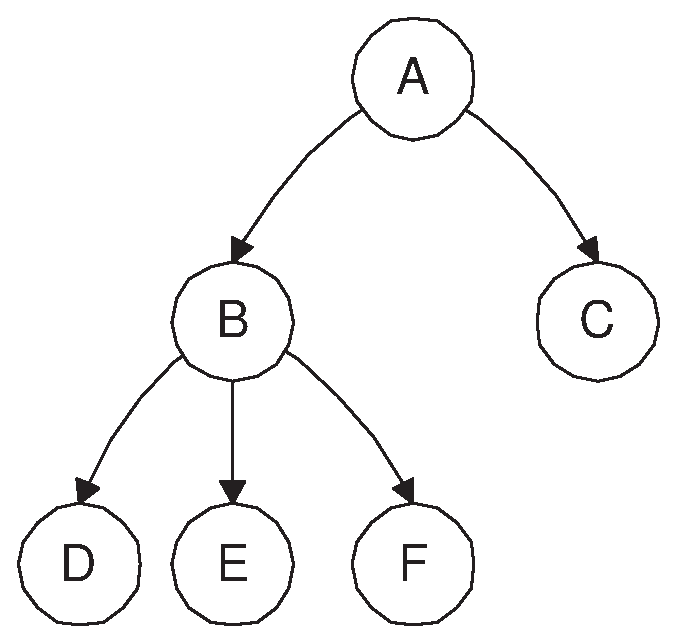
\includegraphics[width=5cm]{./figures/language_tree_example.eps}
\caption{Structuring example}
\label{fig:language:tree_example}
\end{center} \end{figure}

\bigskip \noindent
Note that the tree in Figure \ref{fig:language:tree_example} contains a
toplevel node (node A), one embedded node (node B) and several leaf nodes (D,
E, F and C). Likewise, the configuration file language distinguishes between
toplevel, embedded and leaf components. The possible components for each of
these categories are discussed in Section \ref{sect:language:uiref}.


\subsection{Component types}
As mentioned earlier, the components in the tree have type and the type
determines what kind of user interface element is created for that component. The types range
from strings and numbers to spreadsheets and sections. A common typing
mechanism is to put the type name in front of the declaration. For example, if we
were to declare an instance of \verb=spreadsheet= type named
\verb=capacitances= this would result in:
\begin{alltt}
spreadsheet \emph{capacitances} \{
    ...
\}
\end{alltt}
In this example, \verb=spreadsheet= is the type of the component and
\texttt{\emph{capacitances}} is the identifier with which this instance can be
referred to. This identifier can be used in the generator specifications to
access the values in the spreadsheet entered by the user.

This approach is very usable and is therefore applied in the configuration file
language.

\subsection{Properties}
Components support properties (see also Section \ref{sect:design:components})
and a mechanism to set the properties of a component should be present in the
language. This can be done in many ways. The obvious way would be to use the
equality sign:
\begin{alltt}
section \emph{conductors} \{
    title = "Conductors list";
\}
\end{alltt}
This approach has a disadvantage however, because this construction looks too
much like an assignment. Assignments are normally used to set the value of an
identifier. This could lead to confusion because identifiers are used to name
the components. The user could think that these identifiers can have values
assigned, for example: \verb|conductors = | \verb|"Conductor list"|. This is
not the case. In the example above \verb=title= is not an identifier that can
have a value assigned, but a property that can have a value set. It is better
to reserve the assignment construction for a future version of the language
that will support these identifier assignments.

A different construction is therefore needed to set property values. The
approach finally taken is to use rounded brackets after the property name.
Inside the brackets is the new value for the property:
\begin{alltt}
section \emph{conductors} \{
    title("Conductors list");
\}
\end{alltt}
This is a more function-like approach. Comma's can be used to add additional
values, like in the example below:
\begin{alltt}
conditionlist \emph{condlist_contacts} \{
    adddatafrom(maskdata_sheet.name, maskdata_sheet.comment);
\}
\end{alltt}
The interpretation of the property values (the ``arguments'') depend on the
context in which they are used. The possibilities are discussed in Section
\ref{sect:language:uiref}.

\subsection{Generators} \label{sect:language:generators_intro}
The technology file generator specifications do not completely ``fit'' into the component mechanism
previously described. The mechanism suffices for naming the generator and setting some
basic properties of the generator, but not for the expression tree that will
evaluate to the generated text.

Because of this, a special component statement is introduced that switches the
parser to a new mode. In this mode, each string is treated as literal text.
Identifiers that point to some part of the user interface evaluate to the value
entered by the user in that part of the user interface. For example:
\begin{alltt}
generator \emph{maskdata_gen} \{
    filename("maskdata");
    title("Maskdata file");

    generate \{
        "# Automatically generated file. Do not edit.\(\backslash\)n"
        "number_of_rows:\t" maksdata_sheet.numrows "\(\backslash\)n"
        "#############################################\(\backslash\)n"
    \}
\}
\end{alltt}
In this example, the \verb=generate= statement switches the parser to the
generator mode. The plain-text and identifier methods are also demonstrated.
Some special constructions are available as well, but these are discussed in
detail in Section \ref{sect:language:generatorref}.

\subsection{Macro definitions} \label{sect:language:macros}
In some cases it is useful if it is possible to define a macro. For example,
condition lists are used in multiple places. An example condition list is given
below:
\begin{alltt}
conditionlist \emph{condlist_simp} \{
    option("noextended");
    adddatafrom(maskdata_sheet.name, maskdata_sheet.comment);
    title("Condition list"); // Default title
\}
\end{alltt}
It would be convenient if there was a way to repeat this condition list without
retyping all properties. This is can be achieved by placing the word
\verb=define= in front of this declaration:
\begin{alltt}
define conditionlist \emph{condlist_simp} \{
    option("noextended");
    adddatafrom(maskdata_sheet.name, maskdata_sheet.comment);
    title("Condition list"); // Default title
\}
\end{alltt}
We can now use this \verb=condlist_simp= as a new component type:
\begin{alltt}
spreadsheet \emph{conductors_sheet} \{
    ...
    condlist_simp \emph{cond_list} \{
        title("Conductor condition list:"); // Overriding or
        align(right);  // adding a property is allowed.
    \}
    ...
\}

spreadsheet \emph{fets_sheet} \{
    ...
    condlist_simp \emph{cond_list} \{
        title("FET condition list:"); // Overriding a
                               // property is allowed.
    \}
    ...
\}
\end{alltt}
The three properties as defined in the macro do not have to be typed again. The
example also demonstrates the possibility to set additional properties like the
\verb=align= property. It is also possible to override a property. This is
demonstrated with the \verb=title= property.

If the \verb=title= property does not need to be redefined an empty block must
be specified with curly braces (\verb=condlist_simp cond_list {}=). To people
with programming experience this can be confusing. They would expect a
semicolon to be sufficient. However, this language construction is already used
in the ``chopping'' mechanism, and using it on a macro reference would result
in undefined behaviour. The ``chopping'' mechanism is explained in Section
\ref{sect:language:chopping}. Perhaps in a next release of the language this
behaviour could be changed.

\bigskip \noindent
Another useful application of this mechanism is in dropdowns or comboboxes. For
example, if the user can choose the accuracy of an algorithm and there are many
algorithms to run:
\begin{alltt}
define dropdown \emph{algo_acc} \{
    item \emph{highest} \{ title("Highest accuracy - longest runtime"); \}
    item \emph{high}    \{ title("High accuracy - long runtime"); \}
    item \emph{normal}  \{ title("Normal accuracy - normal runtime"); \}
    item \emph{low}     \{ title("Low accuracy - short runtime"); \}
    item \emph{lowest}  \{ title("Lowest accuracy - shortest runtime"); \}
\}

paramlist \emph{algo_params} \{
    algo_acc \emph{alg_A} \{ title("Algorithm A accuracy:"); \}
    algo_acc \emph{alg_B} \{ title("Algorithm B accuracy:"); \}
    ...
\}
\end{alltt}
This mechanism could also be used for yes/no or on/off dropdowns. One could
argue that these kind of macros should be built-in in the language. The choice
was made not to do this. This is the first version of the language and it has not
been released to a large public. The interface should therefore be kept as
clean as possible. A future version of the language could easily implement
these built-ins if the need for them arises.

\bigskip \noindent
Nesting of macros is allowed. This means it is possible to use a defined type
inside another macro.

\bigskip \noindent
\paragraph{Implementation\\ }
\noindent Whenever the parser encounters a situation in which a previously declared
\verb=define= is used, it copies the branch of the component tree of the
\verb=define= to the correct location. If any properties were added or changed
like in the first example it updates the copied branch of the component tree to
reflect these changes.

Note that the parser performs on-the-fly disambiguation for macro definitions.
This means a macro must be defined before it is used.

\subsection{Reducing indentation} \label{sect:language:chopping}
As was mentioned earlier, indentation with whitespace is not necessary. However, it
is encouraged because it increases the readability of the configuration file.
If the number of nestings becomes too large though, this readability can decrease again. The
indentation then becomes too large.

To counter this effect, a ``chopping'' mechanism is introduced. Chopping makes
it possible to place declarations outside the hierarchy if desired. For
example, a tabpage usually consists of a scrollframe with several sections:
\begin{alltt}
tabpage \emph{element_definition} \{
    scrollframe \emph{element_def_frame} \{
        section \emph{fets} \{
            spreadsheet \emph{fets_sheet} \{
                ...
            \}
            ...
        \}
        section \emph{bjts} \{
            spreadsheet \emph{bjts_sheet} \{
                ...
            \}
            ...
        \}
        ...
    \}
\}
\end{alltt}
Even in this little example the indentation becomes considerable. The
``chopping'' mechanism is demonstrated below:
\begin{alltt}
section \emph{fets} \{
    spreadsheet \emph{fets_sheet} \{
        ...
    \}
    ...
\}

section \emph{bjts} \{
    spreadsheet \emph{bjts_sheet} \{
        ...
    \}
    ...
\}

tabpage \emph{element_definition} \{
    scrollframe \emph{element_def_frame} \{
        section \emph{fets};
        section \emph{bjts};
        ...
    \}
\}
\end{alltt}
This way, the tabpage declaration remains clear because the finer details are
``hidden'' in the sections.

This method is called ``chopping'' because a branch of the component tree is
cut off, leaving a reference at the location the chopping occurred.

\subsubsection*{Differences with macro definitions}
The main differences are listed below:
\begin{itemize}
\item References to macros can be used many times. References to a chopped branch
can be used only once. If used more than once, the resulting behaviour is
undefined.
\item References to chopped branches use a different syntax than references to
defined macros. A reference to a define macro uses the macro name and must be
followed by block markers (\{ ... \}). A reference to a chopped branch must be
followed by a semicolon. If a reference to a branch is followed by block
markers the resulting behaviour is undefined. If a reference to a macro is
followed by a semicolon the resulting behaviour is undefined. As was mentioned
in Section \ref{sect:language:macros}, the syntactical difference between an
empty macro (no additions or overrides, \verb={ }=) and a chopped bracn can be
confusing for experienced programmers. However, it should be noted that chopped
branches cannot have additional or overridden properties. Hence, there is no
need for curly braces and a semi-colon suffices. In the case of a macro without
added or overridden properties, the empty curly braces indicate that something
\emph{could} be changed if desired.

As was already mentioned in Section \ref{sect:language:macros}, changing the
syntax of these constructions should be considered in a next release.
\end{itemize}

\bigskip \noindent
Like the macro definition, nested choppings are allowed. This means that in the
example it is allowed to chop the \texttt{scrollframe
\emph{element\_def\_frame}} as well.

\subsubsection*{Implementation}
If we look at it from a tree perspective, defined macro branches are
\emph{copied} to new locations in the tree while the chopped of branches are
\emph{moved} back to the position where they belong. This is done by
the parser. Whenever the parser encounters a reference to a chopped of branch,
it tries to find the chopped of branch and moves it to the correct position in
the component tree.

Note that the parser performs on-the-fly disambiguation for chopped branches,
just like it does for macro definitions. This means the chopped branch must be
put before the reference to it.

\subsection{Data connections}
The data connections as discussed in Section \ref{sect:design:dataconnections}
must have a place in the language as well. A data connection consist of one or
more sources linked to a single target. Therefore, the most logical place to
define a data connection would be inside the target component. If we make a
data connection declaration a property, we can also use the
\verb=CFindPropertyVisitor= class to find them when the data connections need
to be built. An example of the implemented construction is given below:
\begin{alltt}
define dropdown \emph{layer} \{
    adddatafrom(maskdata_sheet.name, layer_synonyms.name);
\}
\end{alltt}
In this example we define a dropdown \verb=layer=. The items in the dropdown
are the \verb=name= column in the spreadsheet \verb=maskdata_sheet= and the
spreadsheet \verb=layer_synonyms=.

The data connections are established right after the \verb=CGUITree= object is
created by the \verb=CGUIBuilderVisitor=.

\bigskip \noindent
The only datasource currently implemented is a column in a spreadsheet. The
currently available data targets can be found in the \verb=adddatafrom= column
of Table \ref{tab:language:overview}.

%\begin{table}[t!]
%\caption{Data targets. Components not present in this table do not support the
%\texttt{adddatafrom} property. }
%\label{tab:language:data_connections}
%\begin{tabular}{l|p{25mm}|p{55mm}}
%\hline
% \textsf{Context} & \textsf{Possible target components} & \verb=adddatatfrom= \textsf{arguments} \\
%\hline
%\verb=spreadsheet=  & \verb=dropdown,= \verb=combobox=  &  Each argument is the unambiguous name of a valid data source.
%                                                             Each cell in the column described by the dropdown or combobox
%                                                             will have the values of the sources specified in the
%                                                             \verb=adddatafrom= argument. The number of arguments (sources)
%                                                             allowed is one or more. The data obtained from the sources is
%                                                             concatenated.\\
%                    & \verb=conditionlist=                & The first argument defines the source for the layer names.
%                                                            The second argument
%                                                            defines the source
%                                                            for the layer
%                                                            descriptions. The first argument is required, the second is optional.\\
%non-spreadsheet   &  \verb=dropdown,= \verb=combobox=  &  Each argument is the
%unambiguous name of a valid data source.
%                                                             The dropdown or combobox will have the values of the sources
%                                                             specified in the \verb=adddatafrom= argument. \\
%\hline
%\end{tabular}
%\end{table}

%%%%%%%%%%%%%%%%%%%%%%%%%%%%%%%%%%%%%%%%%%%%%%%%%%%%%%%%%%%%%%%%%%%%%%%%%%%%%
\section{Language overview for user interface elements
\label{sect:language:uiref}}
This section will present all the component types that can be used to create a
user interface. The context in which a certain component type is used
determines what kind of user interface element is created. The context also
affects how a component's properties are used.

Since the context largely determines what will happen, the descriptions of the
component types and their properties are given relative to the context in which
they can be used.

As was mentioned in Section \ref{sect:language:structuring}, we can distinguish
between toplevel, embedded and leaf components. Table
\ref{tab:language:top_leaf} lists which component types belong to which
category.

\begin{table} \begin{center}
\caption{Classification of components.}
\label{tab:language:top_leaf}
\begin{tabular}{l|p{6cm}}
\hline
 \textsf{Classification} & \textsf{Component type(s)} \\
\hline
toplevel     & \verb=tabpage= \\
embedded     & \verb=dropdown,= \verb=combobox,= \verb=spreadsheet,= \verb=section,= \verb=paramlist,= \verb=scrollframe=  \\
leaf         & \verb=integer,= \verb=real,= \verb=string,= \verb=identifier,= \verb=conditionlist=, \verb=color,= \verb=dalistyle=, \verb=item= \\
\hline
\end{tabular} \end{center} \end{table}

The components that can provide a context are the top level and embedded
components. Leaf components cannot provide context, but their interpretation
strongly depends on the context in which they are used.

\bigskip \noindent
In the following subsections, all the context-providing component types are
presented. The interpretation of the components inside the context being
discussed is explained in these subsections. Small examples with their
resulting user interface are given as well. At the end of this section, a
complete overview of the currently possible combinations of context, component
types and properties is presented in Table \ref{tab:language:overview}

\bigskip \noindent
\textbf{Note:} Although it is possible to place components \emph{visually} on
the top level (because of the chopping mechanism described in Section
\ref{sect:language:chopping}), the components \emph{as seen after parsing}
still adhere to the classification presented in Table
\ref{tab:language:top_leaf}.

%\subsection{Leaf components}
%The leaf components can be divided into numbers (\verb=real= and
%\verb=integer=), text types (\verb=string=, \verb=identifier=,
%and \verb=conditionlist=) and color/fill style types (\verb=color= and
%\verb=dalistyle=). The actual widget that will be created for them depends on
%the context in which they are found. Also, not every context is applicable. For
%example, when a \verb=string= is encountered inside a \verb=paramlist= the
%widget will be a \verb=QLineEdit=. If it is encountered inside a spreadsheet,
%it will become a column of that spreadsheet.

\subsection{Components in a dropdown or combobox context }
The dropdown is used exactly the same as the combobox. The only difference is
in the behaviour of the widget that will be created. Dropdown widgets present
the user with a fixed list of choices. The combobox widget also presents a list
of choices. However, the user can also enter text not present in the list of
available choices. Because of the similarities we will only discuss the
dropdown.

\bigskip \noindent
The dropdown can only have \verb=item= children inside. All items will become
entries in the dropdown widget. Each item must have the \verb=title= property
set to the text that will be displayed as the entry in the dropdown widget. If
the \verb=title= property of an item is not specified, an empty entry will be
inserted in the dropdown.
%%%\small
%%%\begin{center}
%%%\begin{tabularx}{\textwidth}{|l|l|X|}
%%%  \hline
%%%  \multicolumn{3}{|l|}{\textsf{List of accepted child components}} \\
%%%  \hline
%%%  \multicolumn{3}{|l|}{Child component type: \texttt{item}} \\
%%%  \hline
%%%  &  \textsf{Property} & \textsf{Description} \\
%%%  \cline{2-3}
%%%  & \texttt{title} & The value of this property will be used as the text of the corresponding entry in the  dropdown. \\
%%%  \cline{2-3}
%%%  & \multicolumn{2}{|X|}{Ignored properties: \mbox{\texttt{hint, default, align, unit, pixmap, option}}} \\
%%%  \cline{2-3}
%%%  & \multicolumn{2}{|X|}{Forbidden properties: \texttt{adddatafrom}} \\
%%%
%%%  \hline
%%%  \multicolumn{3}{|X|}{Using forbidden properties or unlisted component types as children will result in undefined behaviour.} \\
%%%  \hline
%%%\end{tabularx}
%%%\end{center}
%%%\normalsize

\paragraph{Example:}
\begin{alltt}
dropdown \emph{def_carr_type} \{
    item \emph{n} \{ title("n doped conductor"); \}
    item \emph{p} \{ title("p doped conductor"); \}
    item \emph{m} \{ title("metal"); \}
    default(\emph{m});
\}
\end{alltt}

\begin{figure}[h!] \begin{center}
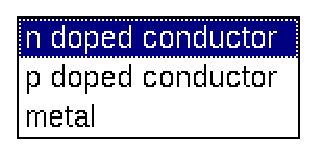
\includegraphics[width=3cm]{./figures/ex_dropdown.eps}
\caption{Dropdown example result.}
\end{center} \end{figure}


%
%\begin{PropTable}
% \verb=default=     & Sets the item that will be displayed by default.  \\
% \verb=hint=        & Sets the hint text that will be displayed when the mouse
%                      hovers over the widget. \\
% \verb=adddatafrom= & Sets this components data sources. Items received from
%                      the source will be added to this dropdown.
%\end{PropTable}

\subsection{Components in a spreadsheet context}
In a spreadsheet, each child is interpreted as a column. The number of rows
changes dynamically, as the user can add or remove rows. The edit mode of the
column corresponds to the columns type. This means a
\verb=string= column corresponds to a \verb=QLineEdit= as edit widget. These
are the types that can be columns in a spreadsheet:
\begin{itemize}
\item \verb=string=, \verb=real=, \verb=integer= and \verb=identifier=
correspond to a column using \verb=QLineEdit= widgets.
\item \verb=color= columns create \verb=CColorCells= that bring up the \verb=QColorDialog= box. They display
the selected color.
\item \verb=dalistyle= columns are edited using the dali colorpicker dialog.
The selected style is displayed in the cells.
\item \verb=conditionlist= columns are edited with the condition list editor.
\item \verb=dropdown= and \verb=combobox= columns display a dropdown
respectively a combobox widget.
\end{itemize}

\paragraph{Example:}
\begin{alltt}
spreadsheet \emph{maskdata_sheet} \{
    integer             \emph{ID} \{ title("Layer ID"); \}
    identifier          \emph{name} \{ title("Layer name"); \}
    def_layer_type      \emph{layertype} \{ title("Layer type"); \} // def_layer_type is a macro
    dalistyle           \emph{dali} \{ title("Dali draw style"); \}
    color               \emph{xspace} \{ title("XSpace draw color"); \}
    string              \emph{comment} \{ title("Comment"); \}
\}
\end{alltt}

\begin{figure}[h!] \begin{center}
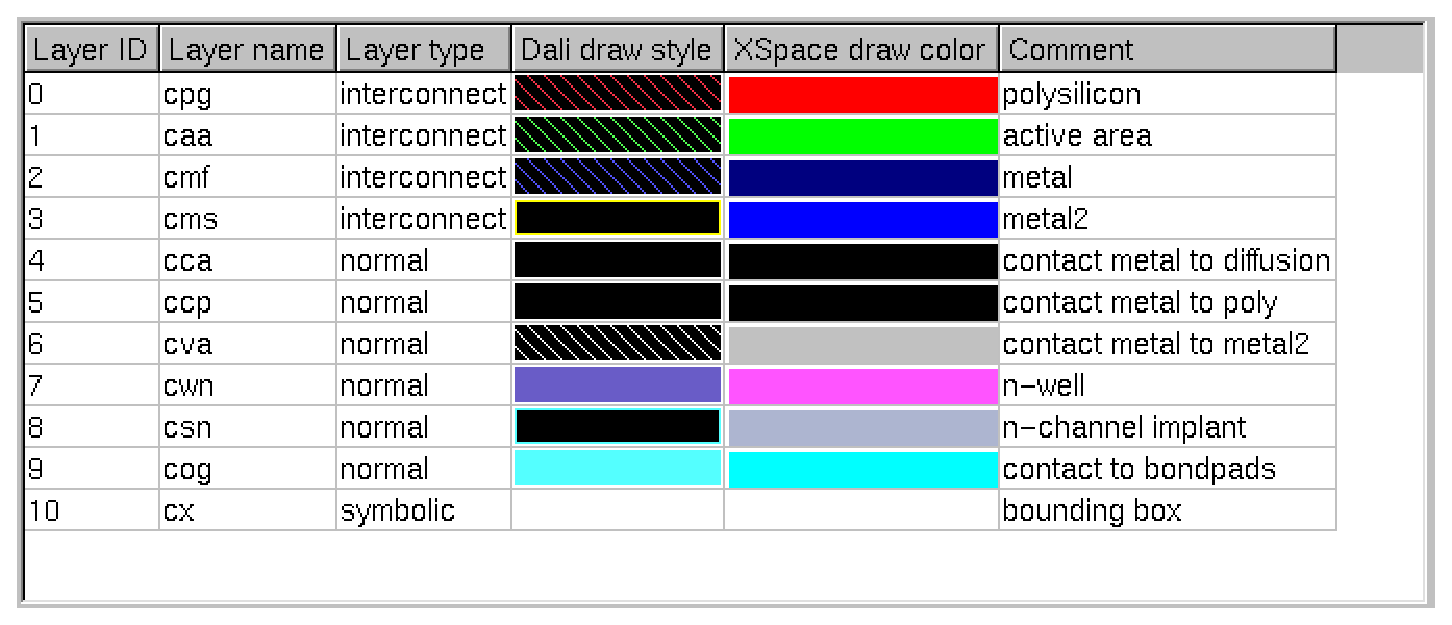
\includegraphics[width=8cm]{./figures/ex_spreadsheet.eps}
\caption{Spreadsheet example result.}
\end{center} \end{figure}

%%%\small
%%%\begin{center}
%%%\begin{tabularx}{\textwidth}{|l|l|X|}
%%%  \hline
%%%  \multicolumn{3}{|X|}{\textsf{List of accepted child components}} \\
%%%  \hline
%%%  \multicolumn{3}{|X|}{Child component type: \texttt{real, integer, identifier, string, color, dalistyle}} \\
%%%  \hline
%%%
%%%  &  \textsf{Property} & \textsf{Description} \\
%%%  \cline{2-3}
%%%  & \texttt{title} & The value of this property will be used as the title of the corresponding column in the spreadsheet. \\
%%%  \cline{2-3}
%%%  & \texttt{default} & The value of this property will be used as default value to display in the spreadsheet cells of this column. \\
%%%  \cline{2-3}
%%%  & \texttt{align} & The value of this property can be \texttt{left, right} or \texttt{center}. This column will be aligned accordingly.\\
%%%  \cline{2-3}
%%%  & \multicolumn{2}{|X|}{Ignored properties: \texttt{hint, unit, pixmap, option}} \\
%%%  \cline{2-3}
%%%  & \multicolumn{2}{|X|}{Forbidden properties: \texttt{adddatafrom}} \\
%%%  \hline
%%%
%%%  \multicolumn{3}{|l|}{Child component type: \texttt{dropdown, combobox}} \\
%%%  \hline
%%%  &  \textsf{Additional properties} & \textsf{Description} \\
%%%  \cline{2-3}
%%%  & \texttt{adddatafrom} & The value of this property should be a reference to a data source. The source data will be used to fill the dropdown.\\
%%%  \cline{2-3}
%%%  & \texttt{default} & The value of this property must be the name of an \texttt{item} child of the dropdown. \\
%%%  \cline{2-3}
%%%  & \multicolumn{2}{|X|}{Ignored properties: \texttt{hint, unit, pixmap, option}} \\
%%%  \hline
%%%
%%%  \multicolumn{3}{|X|}{Child component type: \texttt{conditionlist}} \\
%%%  \hline
%%%  &  \textsf{Additional properties} & \textsf{Description} \\
%%%  \cline{2-3}
%%%  & \texttt{adddatafrom} & Accepts two property values. They must be references to a data source. The first value of this property will be used as the condition list layer names. This value is mandatory. The second value of this property will be used for the layer descriptions and is optional. The layer descriptions are used as explanation of the (short) layer names. If the first property value is not specified, the behaviour is undefined.\\
%%%  \cline{2-3}
%%%  & \texttt{option} & The value of this property can be either \verb=extended= or \verb=noextended=. Using verb=extended= shows the condition list dialog with three columns: `one side', `tile' and 'other side'. Using \verb=noextended= will only show the `tile' column.\\
%%%  \cline{2-3}
%%%  & \multicolumn{2}{|X|}{Ignored properties: \texttt{hint, unit, pixmap, option}} \\
%%%  \hline
%%%
%%%  \multicolumn{3}{|X|}{Using forbidden properties or unlisted component types as children will result in undefined behaviour.} \\
%%%  \hline
%%%\end{tabularx}
%%%\end{center}
%%%\normalsize

%\begin{PropTable}[Description of useful child properties:]
% \verb=title=       & Use the \verb=title= property to set the column title. \\
% \verb=align=       & Use the \verb=align= property to set the alignment of the
%                      column. Possible values are \verb=left=, \verb=right= and \verb=center=. \\
% \verb=adddatafrom= & Only available if the child supports data connections.
%\end{PropTable}
%\clearpage

\subsection{Components in a paramlist context}
The parameter list displays a three column widget. The first column contains
descriptions of the input fields, the middle column contains the input widgets
and the last column can contain additional text, for example to display the
unit of the value that must be entered.

The children of the \verb=paramlist= component can be any type. The most useful
types are the \verb=string=, \verb=real=, \verb=integer=, \verb=dropdown= and
\verb=combobox= types.

%%%\small
%%%\begin{center}
%%%\begin{tabularx}{\textwidth}{|l|l|X|}
%%%  \hline
%%%  \multicolumn{3}{|X|}{\textsf{List of accepted child components}} \\
%%%  \hline
%%%
%%%  \multicolumn{3}{|X|}{Child component type: \texttt{real, integer, identifier, string, spreadsheet}} \\
%%%  \hline
%%%  &  \textsf{Property} & \textsf{Description} \\
%%%  \cline{2-3}
%%%  & \texttt{title} & The value of this property will be used as the label in the first column. \\
%%%  \cline{2-3}
%%%  & \texttt{hint} & The value of this property will be shown as a hint text as the mouse ``hovers'' over the widget in the second column. The hint text can be split over multiple lines by inserting $\backslash$n at the right places. \\
%%%  \cline{2-3}
%%%  & \texttt{default} & The value of this property will be used as the default value to display in the widget (ignored for spreadsheets). \\
%%%  \cline{2-3}
%%%  & \texttt{unit} & The value of this property will be used as the label in the third column. \\
%%%  \cline{2-3}
%%%
%%%  & \multicolumn{2}{|X|}{Ignored properties: \mbox{\texttt{align, pixmap, option}}} \\
%%%  \cline{2-3}
%%%  & \multicolumn{2}{|X|}{Forbidden properties: \texttt{adddatafrom}} \\
%%%  \hline
%%%
%%%  \multicolumn{3}{|l|}{Child component type: \texttt{dropdown}} \\
%%%  \hline
%%%  &  \textsf{Additional properties} & \textsf{Description} \\
%%%  \cline{2-3}
%%%  & \texttt{adddatafrom} & The value of this property is a reference to the data source. The data from the source is used as the entries in this dropdown. \\
%%%  \cline{2-3}
%%%  & \texttt{default} & The value of this property must be the name of an \texttt{item} child of the dropdown. \\
%%%  \cline{2-3}
%%%
%%%  & \multicolumn{2}{|X|}{Ignored properties: \mbox{\texttt{align, pixmap, option}}} \\
%%%  \cline{2-3}
%%%
%%%  \hline
%%%  \multicolumn{3}{|X|}{Using forbidden properties or unlisted component types as children will result in undefined behaviour.} \\
%%%  \hline
%%%\end{tabularx}
%%%\end{center}
%%%\normalsize

%\begin{PropTable}[Description of useful child properties:]
% \verb=title=       & Use the \verb=title= property to set the text in the first
%                      column. \\
% \verb=unit=        & Use the \verb=unit= property to set the text in the last
%                      column. \\
% \verb=hint=        & Sets the hint text that will be displayed when the mouse
%                      hovers over the widget. \\
% \verb=adddatafrom= & Only available if the child supports data connections.
%\end{PropTable}

\paragraph{Example:}
\begin{alltt}
paramlist \emph{units_list} \{
    real \emph{resistance} \{
        title("Sheet resistance unit:");
        unit("in ohm");
        hint("You can specify a base for the values you \(\backslash\)n"
             "will enter below. Use as follows:\(\backslash\)n"
             "If you do not want to type 3e-6, 8e-6 12.5e-6, etc.\(\backslash\)n"
             "but 3, 8, 12.5 instead, type 1e-6 here.");
    \}
    dropdown \emph{accur} \{
        title("Accuracy:");
        item \emph{low} \{ title("Low accuracy"); \}
        item \emph{normal} \{ title("Normal accuracy"); \}
        item \emph{high} \{ title("High accuracy"); \}
        default(\emph{normal});
    \}
\}
\end{alltt}

\begin{figure}[h!] \begin{center}
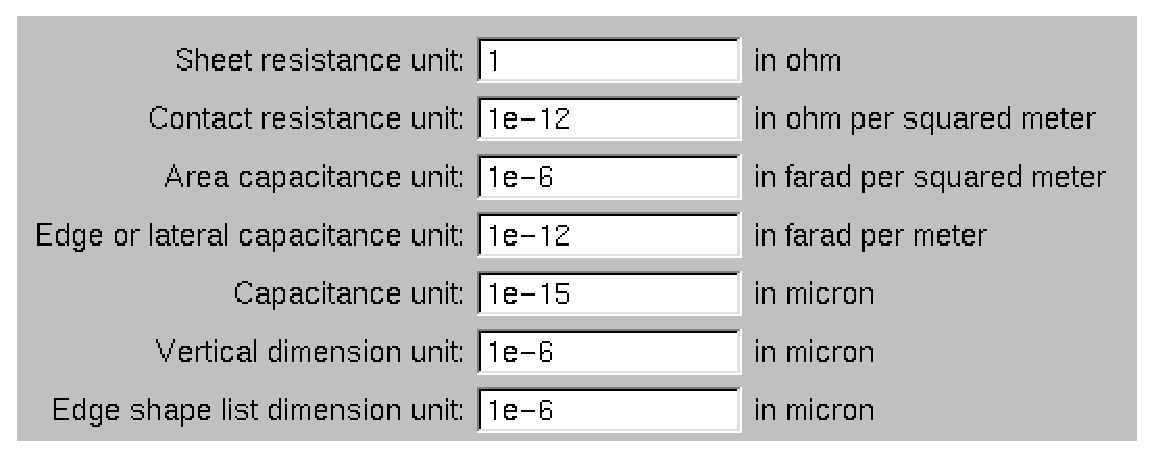
\includegraphics[width=8cm]{./figures/ex_paramlist.eps}
\caption{Parameter list example result.}
\end{center} \end{figure}


%\subsection{Condition list components}
%A condition list component can only be used inside a spreadsheet. The edit mode
%of this type of cell brings up the condition list editor. The condition list
%editor is described in Section \ref{sect:uidesign:conditionlist}.
%
%The condition list component relies on two properties: \verb=adddatafrom= and
%\verb=option=. They are described in the table below.
%\begin{PropTable}[Condition list component properties]
% \verb=title=       & Use the \verb=title= property to set the column title. \\
% \verb=align=       & Use the \verb=align= property to set the alignment of the
%                      column. Possible values are \verb=left=, \verb=right= and \verb=center=. \\
% \verb=adddatafrom= & The first data source specified is used for the layer
%                      names. It must be set for the editor to make sense. The
%                      second data source is used for the layer descriptions and
%                      is optional. \\
% \verb=options=     & The options property can be set to \verb="noextended"= or
%                      to \verb="extended"=. If option extended is specified, the
%                      editor will display the ``one side'' and ``other'' side
%                      button columns.
%\end{PropTable}
%
%\paragraph{Example:}
%\begin{alltt}
%define conditionlist \emph{condlist_ext} \{
%    option("extended");
%    adddatafrom(maskdata_sheet.name, maskdata_sheet.comment);
%\}
%\end{alltt}
%\noindent This example defines a new type that represents an extended condition
%list. This way, the \verb=option("extended")= and \verb=adddatafrom= properties
%do not have to be specified every time a condition list is used.

\subsection{Components in a section context}
Sections are best used inside scrollframes because the total area they can
cover can become quite large. The children of a section are placed vertically
inside the sections expand/collapse area.

%\begin{PropTable}
% \verb=title=       & Use the \verb=title= property to set the title. \\
% \verb=hint=        & Sets the hint text that will be displayed when the mouse
%                      hovers over the section bar. \\
% \verb=pixmap=      & An optional icon to display between the button and the
%                      section label.
%\end{PropTable}

%%%\small
%%%\begin{center}
%%%\begin{tabularx}{\textwidth}{|l|l|X|}
%%%  \hline
%%%  \multicolumn{3}{|X|}{\textsf{List of accepted child components}} \\
%%%  \hline
%%%
%%%  \multicolumn{3}{|X|}{Child component type: \texttt{real, integer, identifier, string, spreadsheet}} \\
%%%  \hline
%%%  &  \textsf{Property} & \textsf{Description} \\
%%%  \cline{2-3}
%%%  & \texttt{hint} & The value of this property will be shown as a hint text as the mouse ``hovers'' over the widget. The hint text can be split over multiple lines by inserting $\backslash$n at the right places. \\
%%%  \cline{2-3}
%%%  & \texttt{default} & The value of this property will be used as the default value to display in the widget (ignored for spreadsheets). \\
%%%  \cline{2-3}
%%%
%%%  & \multicolumn{2}{|X|}{Ignored properties: \mbox{\texttt{title, align, pixmap, option, unit}}} \\
%%%  \cline{2-3}
%%%  & \multicolumn{2}{|X|}{Forbidden properties: \texttt{adddatafrom}} \\
%%%  \hline
%%%
%%%  \multicolumn{3}{|l|}{Child component type: \texttt{dropdown}} \\
%%%  \hline
%%%  &  \textsf{Additional properties} & \textsf{Description} \\
%%%  \cline{2-3}
%%%  & \texttt{adddatafrom} & The value of this property is a reference to the data source. The data from the source is used as the entries in this dropdown. \\
%%%  \cline{2-3}
%%%  & \texttt{default} & The value of this property must be the name of an \texttt{item} child of the dropdown. \\
%%%  \cline{2-3}
%%%
%%%  & \multicolumn{2}{|X|}{Ignored properties: \mbox{\texttt{align, pixmap, option}}} \\
%%%  \cline{2-3}
%%%
%%%  \hline
%%%  \multicolumn{3}{|X|}{Using forbidden properties or unlisted component types as children will result in undefined behaviour.} \\
%%%  \hline
%%%\end{tabularx}
%%%\end{center}
%%%\normalsize

\paragraph{Example:}
\begin{alltt}
section \emph{getepslay_body} \{
    title("Individual mask plotting styles");
    spreadsheet \emph{getepslay_sheet} \{
        layer_combo \emph{mask_name} \{ title("Mask"); \}
        string      \emph{pattern} \{ title("Pattern"); \}
        real        \emph{scale} \{ title("Scale"); default("1.0"); \}
        real        \emph{linewidth} \{ title("Linewidth in lambda's"); \}
    \}
\}
\end{alltt}

\begin{figure}[h!] \begin{center}
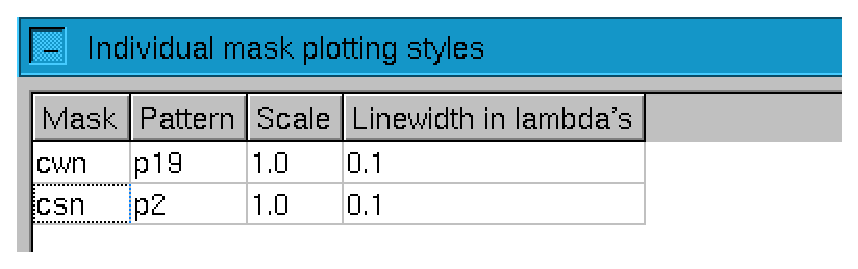
\includegraphics[width=7cm]{./figures/ex_section.eps}
\caption{Section example result.}
\end{center} \end{figure}


\subsection{Components in a scrollframe context}
A scrollframe component is useful primarily inside tabpages. The scrollframe
will then occupy the entire tabpage area, maximizing the area available to the
components inside the frame. Using multiple scrollframes inside a tabpage or
nesting scrollframes is not allowed. This is a limitation in the current
scrollframe implementation. The resulting behaviour is undefined.

There are no properties for the scrollframe itself, because the scrollframe is
not really a visible widget and the behaviour is fixed. Future versions could
implement some properties to influence the behaviour. Examples could be
properties to influence the used layout mechanism (horizontal/vertical) or
child alignment (for example to center or right-justify the widgets instead of
the current left justification).

%%%\small
%%%\begin{center}
%%%\begin{tabularx}{\textwidth}{|l|l|X|}
%%%  \hline
%%%  \multicolumn{3}{|X|}{\textsf{List of accepted child components}} \\
%%%  \hline
%%%
%%%  \multicolumn{3}{|X|}{Child component type: \texttt{real, integer, identifier, string, spreadsheet}} \\
%%%  \hline
%%%  &  \textsf{Property} & \textsf{Description} \\
%%%  \cline{2-3}
%%%  & \texttt{hint} & The value of this property will be shown as a hint text as the mouse ``hovers'' over the widget. The hint text can be split over multiple lines by inserting $\backslash$n at the right places. \\
%%%  \cline{2-3}
%%%  & \texttt{default} & The value of this property will be used as the default value to display in the widget (ignored for spreadsheets). \\
%%%  \cline{2-3}
%%%
%%%  & \multicolumn{2}{|X|}{Ignored properties: \mbox{\texttt{title, align, pixmap, option, unit}}} \\
%%%  \cline{2-3}
%%%  & \multicolumn{2}{|X|}{Forbidden properties: \texttt{adddatafrom}} \\
%%%  \hline
%%%
%%%  \multicolumn{3}{|l|}{Child component type: \texttt{dropdown}} \\
%%%  \hline
%%%  &  \textsf{Additional properties} & \textsf{Description} \\
%%%  \cline{2-3}
%%%  & \texttt{adddatafrom} & The value of this property is a reference to the data source. The data from the source is used as the entries in this dropdown. \\
%%%  \cline{2-3}
%%%  & \texttt{default} & The value of this property must be the name of an \texttt{item} child of the dropdown. \\
%%%  \cline{2-3}
%%%
%%%  & \multicolumn{2}{|X|}{Ignored properties: \mbox{\texttt{align, pixmap, option}}} \\
%%%  \cline{2-3}
%%%
%%%
%%%  \multicolumn{3}{|l|}{Child component type: \texttt{section}} \\
%%%  \hline
%%%  &  \textsf{Properties} & \textsf{Description} \\
%%%  \cline{2-3}
%%%  & \texttt{title} &  The value of this property is displayed in the title bar of the section. \\
%%%  \cline{2-3}
%%%  & \texttt{hint} &  The value of this property will be shown as a hint text as the mouse ``hovers'' over the section. The hint text can be split over multiple lines by inserting $\backslash$n at the right places.\\
%%%  \cline{2-3}
%%%  & \texttt{pixmap} &  The value of this property is the filename of a file containing a pixmap. The filename must be given relative to the \texttt{ICONPATH} specified at the top of the configuration file. The \texttt{ICONPATH} can only contain a single path (for example: \texttt{ICONPATH = "\$(ICDPATH)/lib/spock"}. Environment variables are expanded.)\\
%%%  \cline{2-3}
%%%
%%%  & \multicolumn{2}{|X|}{Ignored properties: \mbox{\texttt{default, align, unit, option}}} \\
%%%  \cline{2-3}
%%%  & \multicolumn{2}{|X|}{Forbidden properties: \texttt{adddatafrom}} \\
%%%  \hline
%%%
%%%  \hline
%%%  \multicolumn{3}{|X|}{Using forbidden properties or unlisted component types as children will result in undefined behaviour.} \\
%%%  \hline
%%%\end{tabularx}
%%%\end{center}
%%%\normalsize

\paragraph{Example:}
\begin{alltt}
scrollframe \emph{element_def} \{
    section \emph{units};
    section \emph{conductors};
    section \emph{fets};
    section \emph{bjts};
    section \emph{connects};
    section \emph{contacts};
    section \emph{capacitances};
\}
\end{alltt}
\noindent This example shows how some section widgets are placed inside a
scrollframe.

\begin{figure}[h!] \begin{center}
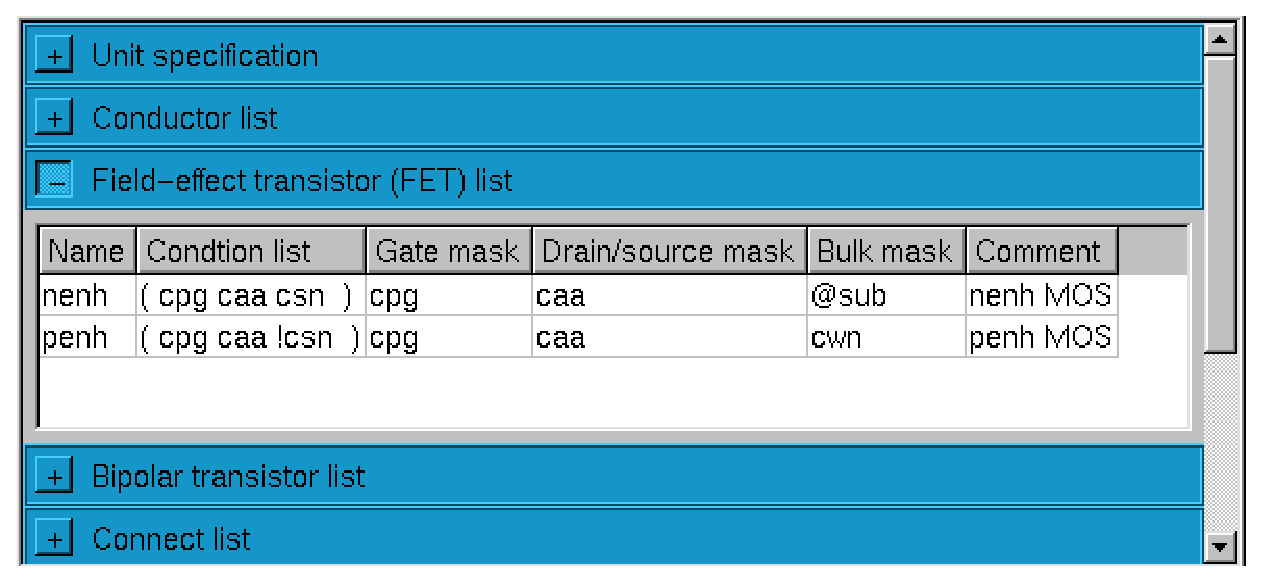
\includegraphics[width=7cm]{./figures/ex_scrollframe.eps}
\caption{Scrollframe example result.}
\end{center} \end{figure}


\subsection{Components in a tabpage context}
Tabpage components will become the tabpages in the user interface. A tabpage
must therefore have a title to distinguish it from the other tabpages.

%\begin{PropTable}
% \verb=title=       & Use the \verb=title= property to set the tabpage label. \\
% \verb=hint=        & Sets the hint text that will be displayed when the mouse
%                      hovers over the tabpage label.
%\end{PropTable}

%%%\small
%%%\begin{center}
%%%\begin{tabularx}{\textwidth}{|l|l|X|}
%%%  \hline
%%%  \multicolumn{3}{|X|}{\textsf{List of accepted child components}} \\
%%%  \hline
%%%
%%%  \multicolumn{3}{|X|}{Child component type: \texttt{real, integer, identifier, string, spreadsheet}} \\
%%%  \hline
%%%  &  \textsf{Property} & \textsf{Description} \\
%%%  \cline{2-3}
%%%  & \texttt{hint} & The value of this property will be shown as a hint text as the mouse ``hovers'' over the widget. The hint text can be split over multiple lines by inserting $\backslash$n at the right places. \\
%%%  \cline{2-3}
%%%  & \texttt{default} & The value of this property will be used as the default value to display in the widget (ignored for spreadsheets). \\
%%%  \cline{2-3}
%%%
%%%  & \multicolumn{2}{|X|}{Ignored properties: \mbox{\texttt{title, align, pixmap, option, unit}}} \\
%%%  \cline{2-3}
%%%  & \multicolumn{2}{|X|}{Forbidden properties: \texttt{adddatafrom}} \\
%%%  \hline
%%%
%%%  \multicolumn{3}{|l|}{Child component type: \texttt{dropdown}} \\
%%%  \hline
%%%  &  \textsf{Additional properties} & \textsf{Description} \\
%%%  \cline{2-3}
%%%  & \texttt{adddatafrom} & The value of this property is a reference to the data source. The data from the source is used as the entries in this dropdown. \\
%%%  \cline{2-3}
%%%  & \texttt{default} & The value of this property must be the name of an \texttt{item} child of the dropdown. \\
%%%  \cline{2-3}
%%%
%%%  & \multicolumn{2}{|X|}{Ignored properties: \mbox{\texttt{align, pixmap, option}}} \\
%%%  \cline{2-3}
%%%
%%%
%%%  \multicolumn{3}{|l|}{Child component type: \texttt{section}} \\
%%%  \hline
%%%  &  \textsf{Properties} & \textsf{Description} \\
%%%  \cline{2-3}
%%%  & \texttt{title} &  The value of this property is displayed in the title bar of the section. \\
%%%  \cline{2-3}
%%%  & \texttt{hint} &  The value of this property will be shown as a hint text as the mouse ``hovers'' over the section. The hint text can be split over multiple lines by inserting $\backslash$n at the right places.\\
%%%  \cline{2-3}
%%%  & \texttt{pixmap} &  The value of this property is the filename of a file containing a pixmap. The filename must be given relative to the \texttt{ICONPATH} specified at the top of the configuration file. The \texttt{ICONPATH} can only contain a single path (for example: \texttt{ICONPATH = "\$(ICDPATH)/lib/spock"}. Environment variables are expanded.)\\
%%%  \cline{2-3}
%%%
%%%  & \multicolumn{2}{|X|}{Ignored properties: \mbox{\texttt{default, align, unit, option}}} \\
%%%  \cline{2-3}
%%%  & \multicolumn{2}{|X|}{Forbidden properties: \texttt{adddatafrom}} \\
%%%  \hline
%%%
%%%  \multicolumn{3}{|l|}{Child component type: \texttt{section}} \\
%%%  \hline
%%%  & \multicolumn{2}{|X|}{The scrollframe is not a visible widget. It does not use any properties.} \\
%%%  \cline{2-3}
%%%  & \multicolumn{2}{|X|}{Ignored properties: \mbox{\texttt{title, hint, default, align, unit, pixmap, option}}} \\
%%%  \cline{2-3}
%%%  & \multicolumn{2}{|X|}{Forbidden properties: \texttt{adddatafrom}} \\
%%%  \hline
%%%
%%%  \hline
%%%  \multicolumn{3}{|X|}{Using forbidden properties or unlisted component types as children will result in undefined behaviour.} \\
%%%  \hline
%%%\end{tabularx}
%%%\end{center}
%%%\normalsize


\paragraph{Example:}
\begin{alltt}
tabpage \emph{getepslay_tab} \{
    title("Postscript plot settings");
    scrollframe \emph{getepslay_frame} \{
        section \emph{getepslay_preamble};
        section \emph{getepslay_body};
    \}
\}
\end{alltt}

\subsection{Overview of combinations}
Table \ref{tab:language:overview} lists the existing relationships between
component types in a certain context and the properties that can be used. Note
that the table lists the \emph{implemented} relationships, not the
\emph{possible} relationships. Additional sensible relationships could be
implemented in a future version of the application.

The numbers in the table refer to the explanations given below. Some numbers
are followed by a letter. The letter \texttt{r} indicates that the property is
required. If these properties are not specified the behaviour of the
application is undefined. The letter \texttt{F} indicates that it is forbidden
to specify that property. If the property is specified anyway, the behaviour of
the application is undefined.

The label \texttt{r.i.s.i.} stands for real, integer, string or identifier. The
row is valid for each of these component types. The combobox type is missing,
but the properties and contexts listed for the dropdown are identical to the
ones listed for the combobox.

If a combination of a component and a context is not listed in the table, the
behaviour resulting from this combination is undefined.

\actd{title1} \actd{title2} \actd{title3} \actd{title4} \actd{hint1}
\actd{hint2} \actd{hint3} \actd{default1} \actd{default2} \actd{align1}
\actd{adddata1} \actd{adddata2} \actd{unit1} \actd{pixmap1} \actd{option1}
\begin{center} \begin{table}
\caption{Combinations of components and properties in a context.}
\label{tab:language:overview}
\small
\begin{tabularx}{\textwidth}{|l|X|c|c|c|c|c|c|c|c|c|c|}
 \hline
 \textsf{Context} & \textsf{Acceptable component types} & \rotated{title} & \rotated{hint} & \rotated{default} & \rotated{align} & \rotated{adddatafrom} & \rotated{unit} & \rotated{pixmap} & \rotated{option} \\
 \hline
 dropdown    & item      & \TR[r]{title1} & & & & F & & & \\ \hline
 spreadsheet & r.i.s.i   & \TR[r]{title2} & & \R{default1} & \R{align1}& F & & & \\ \cline{2-10}
%             & integer   & \TR[r]{title2} & & \R{default1} & \R{align1}& F & & & \\ \cline{2-10}
%             & string    & \TR[r]{title2} & & \R{default1} & \R{align1}& F & & & \\ \cline{2-10}
%             & identifier& \TR[r]{title2} & & \R{default1} & \R{align1}& F & & & \\ \cline{2-10}
             & color     & \TR[r]{title2} & & \R{default1} & & F & & & \\ \cline{2-10}
             & dalistyle & \TR[r]{title2} & & \R{default1} & & F & & & \\ \cline{2-10}
             & conditionlist & \TR[r]{title2} & & & \R{align1} & \TR[r]{adddata1} & & & \R{option1} \\ \hline
 section     & r.i.s.i.  & & \R{hint1} & \R{default1} &  &  F & & & \\ \cline{2-10}
             & dropdown  & & \R{hint1} & \R{default1} &  &  \R{adddata2} & & & \\ \cline{2-10}
             & spreadsheet & & \R{hint1} & & & F & &  & \\ \hline
 paramlist   & r.i.s.i   & \R{title3} & \R{hint2} & \R{default1} & & F & \R{unit1} &  & \\ \cline{2-10}
             & dropdown  & \R{title3} & \R{hint2} & \R{default2} & & \R{adddata2} & \R{unit1} & &  \\ \cline{2-10}
             & spreadsheet & \R{title3} & \R{hint2} & & & F & \R{unit1} & &  \\ \hline
 scrollframe & r.i.s.i.  & & \R{hint1} & \R{default1} & & F & & &  \\ \cline{2-10}
             & dropdown  & & \R{hint1} & \R{default2} &  &  \R{adddata2} & & & \\ \cline{2-10}
             & spreadsheet & & \R{hint1} & & & F & & &  \\ \cline{2-10}
             & section   & \R{title4}& \R{hint3} & & & & & \R{pixmap1} & \\ \hline
 tabpage     & r.i.s.i.  & & \R{hint1} & \R{default1} & & F  & & & \\ \cline{2-10}
             & dropdown  & & \R{hint1} & \R{default2} &  &  \R{adddata2} & & & \\ \cline{2-10}
             & spreadsheet & & \R{hint1} & & & F & & &   \\ \cline{2-10}
             & section   & \R{title4}& \R{hint3} & & & & & \R{pixmap1} & \\ \cline{2-10}
             & scrollframe & & & & & & & & \\ \hline
\end{tabularx}
\normalsize \end{table} \end{center}

The numbers in Table \ref{tab:language:overview} are explained below:\small
\begin{itemize}
\item[\R{title1}] The value of this property will be used as the text of the corresponding entry in the dropdown.
\item[\R{title2}] The value of this property will be used as the title of the corresponding column in the spreadsheet.
\item[\R{title3}] The value of this property will be used as the label in the first column of the parameter list.
\item[\R{title4}] The value of this property will be used as the title displayed in the section bar.
\item[\R{hint1}] The value of this property will be shown as a hint text as the mouse ``hovers'' over the widget. The hint text can be split over multiple lines by inserting $\backslash$n at the right
places. Quotation marks can be inserted with
\texttt{$\backslash$"}.
\item[\R{hint2}] The value of this property will be shown as a hint text as the mouse ``hovers'' over the widget in the second column. The hint text can be split over multiple lines by inserting $\backslash$n at the right
places. Quotation marks can be inserted with
\texttt{$\backslash$"}.
\item[\R{hint3}] The value of this property will be shown as a hint text as the mouse ``hovers'' over the section bar. The hint text can be split over multiple lines by inserting $\backslash$n at the right
places. Quotation marks can be inserted with
\texttt{$\backslash$"}.
\item[\R{default1}] The value of this property will be used as default value to display in the spreadsheet cells of this column.
\item[\R{default2}] The value of this property must be the name of one of the
child items. This item will be shown as the default value in the
dropdown/combobox.
\item[\R{align1}] The value of this property can be \texttt{left, right} or \texttt{center}. The spreadsheet column will be aligned accordingly.
\item[\R{adddata1}] This property accepts two values. Both values must be
identifiers that can be unambiguously resolved. The data referenced by the
first (required) identifier will be used for the layer names in the
conditionlist. The second (optional) identifier references the layer
descriptions.
\item[\R{adddata2}] This property accepts one or more values. Each value is an
identifier that can be unambiguously resolved. The data referenced by each
identifier will be concatenated and the result will become the entries in the
dropdown/combobx.
\item[\R{unit1}] The value of this property will be used as the label in the third column of the parameter
list, after the input field.
\item[\R{pixmap1}] The value of this property is the filename of a file
containing a pixmap. The filename must be given relative to the
\texttt{ICONPATH} specified at the top of the configuration file. The
\texttt{ICONPATH} can only contain a single path (for example: \texttt{ICONPATH
= "\$(ICDPATH)/lib/spock"}. Environment variables are expanded and can be
specified \texttt{Makefile} style: between parenthesis preceded by a \$.)
\item[\R{option1}] This property value must be either \texttt{extended} or
\texttt{noextended}. If \texttt{extended} is specified, the conditionlist
editor is shown with three columns: `one side', `tile' and `other side'. If
\texttt{noextended} is specified, only the `tile' column will be displayed.
\end{itemize}
\normalsize


%%%%%%%%%%%%%%%%%%%%%%%%%%%%%%%%%%%%%%%%%%%%%%%%%%%%%%%%%%%%%%%%%%%%%%%%%%%%%
\section{Language overview for generators} \label{sect:language:generatorref}
This section will present and explain the generator specification in the
configuration file language. The generator specification is put into an
expression tree that evaluates to the contents of the technology files.

The generator component is described first in Section
\ref{sect:language:generator_components}. After that, the use of value mappings
is explained in Section \ref{sect:language:valmaps}. The sections following
Section \ref{sect:language:valmaps} describe the expressions that can be used
inside the \verb=generate= context.

\subsection{Generator components} \label{sect:language:generator_components}
The generator components are specified the same way as the other components in
the configuration file. An example was already given in Section
\ref{sect:language:generators_intro} and is repeated below:
\begin{alltt}
generator \emph{maskdata_gen} \{
    filename("maskdata");
    title("Maskdata file");

    generate \{
        "# Automatically generated file. Do not edit.\(\backslash\)n"
        "number_of_rows:\t" maksdata_sheet.numrows "\(\backslash\)n"
        "#############################################\(\backslash\)n"
    \}
\}
\end{alltt}
The generator type component uses a language construction similar to the other
component types. Like the other component types, properties can be used and the
declaration syntax is the same. However, this component is not translated into
a user interface element. More importantly, additional language constructions
can be used inside the generator component.

The additional language constructions that can be used are the value mappings
and the \verb=generate= statement. The expressions describing the technology
file format must be put inside the generate statement

\begin{PropTable}[The properties supported by the generator component:]
 \verb=title=       & Use the \verb=title= property to set a short descriptive name
                      for the generator. This descriptive name is used in several places in the application, for example in the technology file generation dialog box.\\
 \verb=filename=    & The filename of the technology file to generate. This is
                      only the filename, not the path. The path is specified by
                      the user in the user interface.
\end{PropTable}

If the \verb=title= property is not specified, the description is an empty
string. If the filename property is not specified, the behaviour of the
application is undefined.

\subsection{Value mappings}\label{sect:language:valmaps}
Besides the properties, the generator component supports value mappings. Value
mappings allow the substitution of text used in the \verb=dropdown= and
\verb=combobox= items to a string in the technology file. This allows the use
of a descriptive text in the user interface and a specialized string in the
generated technology file. An example of the construction is given below. The
\verb=dropdown= used in the substitution is also shown to illustrate the
mechanism.

\begin{alltt}
define combobox \emph{def_carr_type} \{
    item \emph{n} \{ title("n doped conductor"); \}
    item \emph{p} \{ title("p doped conductor"); \}
    item \emph{m} \{ title("metal"); \}
    default(\emph{m});
\}

map \emph{def_carr_type} \{
    n = "n";
    p = "p";
    m = "m";
\}
\end{alltt}

The value mapping could of course be extended into a more general mechanism
that allows arbitrary substitutions. This would increase the flexibility of the
generators.

Looking at the example above, one could argue that the identifier name could be
used as a substitution. This has however, as a disadvantage that it would not
be possible to substitute a text that is not an identifier, meaning spaces or
other special symbols could not be used.

\subsection{Literal text}
Use quotation marks to generate literal text. Literal text may contain tabs and
newlines like in C++ using \verb=\t= and \verb=\n=. If quotation marks are
needed they too can be escaped (\verb=\"=). Concatenation of strings can be
used to span long literals over several lines. This is illustrated in the
example below.

\begin{verbatim}
generate {
    "Literal text must be placed between quotation marks (\").\n"
    "\n and \t can be used like in C++. Bordering "
    "literals "   "are "   "concatenated in the output of "
    "the generator."
}
\end{verbatim}

\subsection{Identifier substitution}
To place values in the generator output we can use the name of any identifier
in the user interface specification. The identifier will be replaced with the
value that is currently entered in the applications' user interface.

\begin{verbatim}
generate {
    "The value of getepslay_pl.mask_order is: "
    getepslay_pl.mask_order "\n"
}
\end{verbatim}

Some component types do not generate any output. These are usually types that
contain other components like the scrollframe and the section components.

\bigskip \noindent
In some cases, not the actual value of identifier is required but some other
property. This is achieved by the use of fields. For example, to generate the
number of layers \verb=maskdata_sheet[numrows]= could be used. The field is
specified between square brackets after the identifier name. The currently
supported fields are listed in Table \ref{tab:language:fieldsupport}

Besides the identifiers present in the user interface specification, there is
also a special identifier called
\verb=application=. This identifier can be used to retrieve values from the
application that are not present in the user interface specification.
\verb=application= is a reserved word. If \verb=application= is inadvertently used as an identifier, the parser will exit
with an error.

\begin{table}[h] \begin{center}
\caption{Supported fields:}
\label{tab:language:fieldsupport}
\begin{tabularx}{\textwidth}{l|l|X}
\hline
 \textsf{Component type} & \textsf{Fields} & \textsf{Description} \\
\hline
\texttt{spreadsheet} & \texttt{numrows} & Is replaced with the number of rows present in the spreadsheet. \\
\texttt{dalistyle}   & \texttt{fill} & Is replaced with the selected dali fill number \\
                     & \texttt{clr}  & Is replaced with the selected dali color number \\
\texttt{application} & \texttt{time} & Is replaced with the current time \\
                     & \texttt{date} & Is replaced with the current date \\
                     & \texttt{processname} & Is replaced with name of the process being generated \\
                     & \texttt{processdesc} & Is replaces with a description of the process being generated \\
\hline
\end{tabularx}
\end{center}\end{table}

\subsection{Number addition and subtraction}
Simple addition and subtraction is also supported. For example:
\begin{verbatim}
generate {
    "The number of layers + 1 = " maskdata_sheet[numrows] + 1
}
\end{verbatim}

The type of the result depends on the type of the operands. Two integer
operands will result in an integer but two reals or a real and a integer will
result in a real.

\subsection{Loops}
For spreadsheets it is necessary to be able to loop over the rows or all values
present in a column of a spreadsheet. To support this, a \verb=foreach= loop is
introduced. The foreach loop has two forms. The first form loops over the rows
and has no loop variable:

\begin{verbatim}
foreach(fets.fets_sheet, row) {
   "    " name ":" cond_list ":" mask_g " " mask_ds
   ":" mask_b " # " comment "\n"
}
 "\n"
\end{verbatim}
\verb=fets.fets_sheet= is a hint context. The identifiers inside the loop body
are first resolved using this context. If that yields no results a normal
disambiguation is tried.

\bigskip \noindent
Besides iterating over spreadsheet rows it is also possible to iterate over the
values present in a column. Each value in that column is enumerated exactly
once:

\begin{alltt}
foreach \$t (conductors_sheet, cond_type) {
    "conductor " \$t "\(\backslash\)n"
}
\end{alltt}

Again, the first argument between the brackets is the hint context. The second
argument is an identifier that is a spreadsheet column. All values in that
column will be enumerated.

The loop variable can be used (here \texttt{\$t}) to access the current value
of an iteration. This makes it possible to nest loops. Each loop variable
corresponds to the current iteration values of each of the loops.

If the \verb=cond_type= column contained the values a, b, a, c, d, and a, the
result would be:
\begin{verbatim}
 conductor a
 conductor b
 conductor c
 conductor d
\end{verbatim}

For an example of some more difficult nested loops please take a look at the
sample \verb=spock.uis= configuration file in Appendix \ref{chapt:samplespock}.

\subsection{Conditionals}
In some cases it is necessary to generate a piece of text conditionally. To be
able to do this, a conditional statement is needed. This is provided by the
\verb=if= statement.

\begin{alltt}
foreach \$t (cap_sheet, cap_type) \{
   foreach \$s (cap_sheet, subtype) \{
        \$t " capacitances " \$s ":\(\backslash\)n"
        "#\(\backslash\)tname:condition_list:type:mask1 [mask2]:capacitivity\(\backslash\)n"
        foreach(capacitances.cap_sheet, row) \{
           if (cap_type == \$t) \{
               if (subtype == \$s) \{
                   "\(\backslash\)t" name ":" cond_list ":" mask_1 " " mask_2 ":" capacitivity "\(\backslash\)t\(\backslash\)t# " comment "\(\backslash\)n"
               \}
           \}
        \}
        "\(\backslash\)n"
   \}
\}
\end{alltt}

%\begin{alltt}
%if (space_params.min_coup_cap != "") \{
%    "min_coup_cap "  space_params.min_coup_cap  "\(\backslash\)n"
%\}
%\end{alltt}

\bigskip \noindent
The possible conditional statements are limited to equal or not equal. The
operators for this are \verb|==| and \verb|!=|. Support for additional
operators could easily be implemented in a future version.

%%%%%%%%%%%%%%%%%%%%%%%%%%%%%%%%%%%%%%%%%%%%%%%%%%%%%%%%%%%%%%%%%%%%%%%%%%%%%
\section{Recommended language extensions} \label{sect:language:extensions}
Language extensions can be grouped into two categories:
\begin{enumerate}
\item extensions to the language itself
\item extensions in the form of new types and properties
\end{enumerate}

\subsection{Language extensions}
The configuration file language is quite complete in functionality. However,
some common language constructions seen in other languages are not yet
possible.
\begin{itemize}
\item \textbf{Operators\\ } Currently only + and -- are supported. It is of
course possible to add multiplication (*), division (/) and more math-like
functions like powers (\verb=^=) and perhaps even \verb=sin()= and
\verb=cos()=. This depends on the need for them of course.
\item \textbf{Conditionals\\ } The conditional \verb=if= statement could be
extended with \verb=else= support and additional comparisons like less then and
greater then (\verb=<= and \verb=>=).
\item \textbf{Loops\\ } The \verb=foreach= loop construction provided is
sufficient for simple loops. It could be useful to implement additional loop
structures like \verb=do-while= or \verb=while-do=.
\item \textbf{Value substitition\\ } The value substitution mechanism provided
by the value maps could be extended to a more general substitution mechanism
that can substitute any string for another.
\item \textbf{Perl\\ } It is also possible to embed perl into the application.
The expressions describing the technology file formats could become a block of
perl source.

This mechanism could even be extended to the complete configuration file.
Special perl functions internally defined by the application could then be
called in the configuration file to build the trees.

The disadvantage of using perl is the addition of a dependency to the
application and the possible compilation difficulties on different platforms.
\end{itemize}

\subsection{New types and properties}
Besides extensions to the language itself, it is also possible to add new types
and properties to the language.
\begin{itemize}
\item \textbf{Layout control\\ } It is possible to add properties or components
that use Qt's widget layout mechanism. There would be more control over the
arrangement of the components in this case (For example a \verb=vbox{}= and
\verb=hbox{}= component that layout their children vertically or horizontally).
\item \textbf{More editors\\ } The addition of types would allow more special
purpose editors like the condition list editor and the dali color picker. A
capacitance value generating editor for example (that could be used to generate
the capacitances in the element definition files). Another editor could be a
``pattern picker'' for the fill patterns used by \verb=getepslay=.
\item \textbf{Additional properties\\ } Additional properties can also be very
useful. For example:
    \begin{itemize}
    \item The Qt \verb=whatis= mechanism could be implemented so a \verb=whatis=
    property can be added. This would enhance the context sensitive help
    available to the end user.
    \item More properties that control the looks of a component could be added,
    for example a \verb=font= property that influences the font used in the
    component or a \verb=background= property to set the background color of a
    component.
    \end{itemize}
\item \textbf{Property warnings\\ } Warnings or errors should be given if
required properties are missing or if forbidden or ignored properties are used
\item \textbf{Better default values\\ } If properties are unspecified but can
be used in a certain context, sensible defaults could be chosen. For example,
if the \verb=title= property of generator component is not given it could use
the filename specified in the \verb=filename= property.
\item \textbf{Better conditional output\\ } In some cases (a good example is the
parameter list) the file generation could be simplified if some built-in
construction is available for empty parameter values. This would avoid long
lists of \verb=if= constructions. This could be implemented by some general
mechanism or a parameter specific mechanism.
\end{itemize}

% conclusion.tex

%% Acceptatie van P.v.E. aantonen.
\chapter{Conclusion}\label{chap:conclusion}
In this final chapter we will compare the resulting application with the
requirements stated in Chapter \ref{chap:demands}.

\subsection*{Platform independence}
%% Prove platfrom independence
By using Qt, the STL (standard template library) and the \verb=gcc= compiler we
have made sure that the tools necessary to compile the application are
available on all target platforms. Both Qt and \verb=gcc= are freely available
for all required platforms. All recent versions of \verb=gcc= include a good
implementation of the STL.

These are not sufficient conditions to \emph{guarantee} platform independence.
However, the areas covered by these tools are usually the areas where platform
independcies arise. The application has been successfully tested on both Linux
and Solaris. Some tests were also performed on HP-UX and no problems were
encountered.

The \verb=makefile= generator tool \verb=tmake= also takes away the need to
manually configure the \verb=makefiles= for each target platform.

\subsection*{Integration with SPACE}
%% Prove integration
Integration with SPACE is available. The application can read the file
describing the processes (\verb=processlist=) in the SPACE process tree and the
user can integrate the generated technology files into the SPACE process tree
if desired. The \verb=processlist= file describing the available processes is
automatically updated to reflect the changes that were made.

Unfortunately, the application cannot read the technology files in the SPACE
process tree, it can only read its own file format.

\subsection*{Technology file generation}
%% Prove file generation
The technology files specified in the requirements can all be generated. These
are:
\begin{itemize}
\item \emph{maskdata}, which defines the layers present in the process and the
colors used to represent them in the programs and their output.
\item \emph{space.xxx.s}, the element definition files used by SPACE.
\item \emph{space.xxx.p}, the parameter files used by space.
\item \emph{bmlist.gds}, which provides a mapping between the GDS layer format and
the format used by SPACE.
\item \emph{xspicerc}, a control file that specifies which models are used for
the devices.
\end{itemize}
It should be noted that the space parameter file \verb=space.xxx.p= cannot be
completely generated yet. Not all of the parameters have been included in the
first version of the configuration file.

\subsection*{The configuration file language}
The configuration file language provides the basic functionality needed. The
language can be made more effective if additional language constructions are
implemented. The language constructions for ``chopping'' and macro definitions
can appear mangled to new users. A different syntax could be considered.

\subsection*{Flexibility}
%% Prove flexibility
Another requirement is the possibility to add new files to the list above or to
change the format of these files in a flexible way. This flexibility has been
achieved by making use of a configuration file. The configuration file contains
the specification of the user interface and the generators that use this user
interface to generate the technology files. These files can be changed without
the need to recompile the application.

Flexibility with regard to the source code has been achieved by using a good
source code documentation application and by using some well-known design
patterns that make understanding the code easier.

\bigskip \noindent
The final conclusion is that the developed application meets the requirements
specified in Chapter \ref{chap:demands}.


% backmatter
\addcontentsline{toc}{chapter}{Bibliography}
\bibliographystyle{alpha}
\bibliography{./biblio}

\appendix
% environment.tex

\chapter{Development environment} \label{chap:environment}
Developing an application is usually done with many tools. Some tools are
required for the development (like the compiler). Other tools increase the
programmers productivity.

\bigskip \noindent
The main goal of this chapter is to present the environment in which the
application was developed. This means the used tools and their interaction will
briefly be discussed.

\bigskip \noindent
First of all, the compiler and the platform will be described. This is followed
by a section on \verb=Makefile= generation. The \verb=Makefile= can be a major
headache to developers, especially if multiple platforms are involved. The
source code has been documented using a tool called Doxygen. A short
description of doxygen is given in Section \ref{chap:env:doxygen}.
%%%%%%%%%%%%%%%%%%%%%%%%%%%%%%%%%%%%%%%%%%%%%%%%%%%%%%%%%%%%%%%%%%%%%%%%%%%%%%
\section{Platform and compiler}
The platforms used most actively during the development of the application are
Solaris and Linux. A few compilations have been done on HP-UX as well and these
presented no problems.

The compiler used was \verb=gcc 2.95.2=. The \verb=gcc= compiler is a free
compiler that is available on practically every platform.
%%%%%%%%%%%%%%%%%%%%%%%%%%%%%%%%%%%%%%%%%%%%%%%%%%%%%%%%%%%%%%%%%%%%%%%%%%%%%%
\section{Makefile generation}
Makefiles are a necessary evil when developing applications on Unix or Linux
platforms. This is because there is no good integrated development environment
(like Visual Studio for Windows) available that works on all the platforms that
need to be supported. This is mainly due to the peculiarities of each platform.

A solution to this problem is \verb=tmake=. \verb=tmake= is a small utility
written by the creators of Qt, Trolltech \cite{Qt}. This utility uses templates
and a small input file containing some options and the sources to generate a
\verb=Makefile=. The templates hide the peculiarities of each platform, thus
establishing a platform independent interface.

Another possibility is to use \verb=autoconf=. The overhead involved with
\verb=autoconf= is larger, though.

As was mentioned above, the \verb=tmake= tool uses templates for the generation
of makefiles. There are templates for recursive makes and projects. It is also
possible to use custom templates. For the development of the application a
custom template was created that supports building library and test
applications in a single run as well as support for lex/flex yacc/bison parser
compilation.

%%%%%%%%%%%%%%%%%%%%%%%%%%%%%%%%%%%%%%%%%%%%%%%%%%%%%%%%%%%%%%%%%%%%%%%%%%%%%%
\section{Doxygen} \label{chap:env:doxygen}
Source code documentation can be generated with \verb=doxygen= \cite{doxygen}.
Another candidate for this position was \verb=kdoc=. However, \verb=kdoc=
forces the documentation completely into the header files, making the header
files unreadable. \verb=Doxygen= allows documentation virtually everywhere,
resulting in clean well-readable source files.

\subsection{Possible output formats}
As an added bonus, \verb=doxygen= can generate the documentation in many
formats:
\begin{itemize}
\item HTML format
\item \LaTeX
\item Man page format
\item Rich Text Format (RTF) which can be read by Microsoft Word
\item XML
\end{itemize}
It can even generate a cgi script that can be used as a search engine to search
through the HTML documentation.

\subsection{Doxygen options}
The output of \verb=doxygen=  can be influenced with the many features present.
It is possible to extract everything, even if the code is undocumented (this
shows you the structure of the source code). It is also possible to extract
only the documented code. Private and static members can be ignored if desired.

To keep the printed source code reference a reasonable size and to save some
trees in general, the documentation was created for documented items only,
leaving out the private methods and members.

\subsection{Collaboration diagrams}
If the \verb=graphviz= package is installed, \verb=doxygen= can make use of
\verb=dot=, which is a part of that package. With \verb=dot= it is possible to
create collaboration diagrams. Some of the diagrams created by \verb=dot= are
used in this report, for example Figure \ref{fig:design:guibuilder_partial}.

%%%%%%%%%%%%%%%%%%%%%%%%%%%%%%%%%%%%%%%%%%%%%%%%%%%%%%%%%%%%%%%%%%%%%%%%%%%%%%
\section{Qt Designer}
Qt Designer became available near the end of the project. It is a user
interface editor like X-Designer. It is possible to click together a dialog box
and generate the source code that builds the dialog box. The technology file
generation dialog box was created with Qt Designer as an experiment.

To use the generated source a new class has to be derived from the generated
class. This derived class implements the desired functionality. In the case of
the technology file generation dialog box this is the \verb=CGenerateDlg=
class.

\bigskip \noindent
The ease with which a user interface can be created with Qt Designer is
remarkable. Qt supports automatic widget layout and with Qt Designer this
becomes even easier then before.

Functionality can easily be added to the dialog boxes designed with Qt
Designer. By using inheritance, the only code that needs to be written is the
code that must provide the needed functionality. This makes Qt Designer a true
rapid application development tool.

The only downside of Qt Designer is that is (currently) only possible to create
widgets and dialog boxes. It is not possible to create an application's
framework.

% testing.tex

\chapter{Testing and debugging the application}
\label{chap:testing}
Testing and debugging applications under development is usually not very
difficult. As soon as the application starts to work with events like signals
and slots debugging can become difficult.

\bigskip \noindent
The main goal of this chapter is to present the testing and debugging methods
used, in particular the way Qt's signal/slot mechanism was debugged.

\bigskip \noindent
Section \ref{chap:testing:cycle} discusses the general test -- debug -- develop
cycle commonly used by the programmer. Section \ref{chap:testing:techniques}
will focus more on the debugging techniques applicable to signal/slot
debugging.

\section{The test -- debug -- develop cycle} \label{chap:testing:cycle}
The general test -- debug -- develop cycle is depicted in Figure
\ref{fig:testing:cycle}. The diagram starts with the applications' source code
at some point in time. This source must be compiled to obtain the executable.
If a typing error was made or a method forgotten to implement, the compiler or
linker will not be successful and the source must be edited. This is usually
due to a simple mistake on the programmers part.

\bigskip \noindent
After the source code has been successfully compiled and linked, the
functionality just added to application needs to be tested. This is represented
by the input of test vectors. What these test vectors are, depends on the
application and the functionality being tested. The tester (in this case the
programmer) then either marks the added functionality as successful or
unsuccessful.

If testing was successful, the programmer can continue to implement the next
feature. If testing failed, a bug is present in the application. The bug must
then be located. The bug is usually related to feature that was added but this
is not necessarily the case (either because of poor testing or because some
other part of the code could not be tested before this part was ready).

\bigskip \noindent
Locating a true bug can be quite difficult. It is usually the most
time-consuming part of development and is therefore shown in grey in the
figure. Once the bug has been identified a solution can be found easily in most
cases. The cycle then continues normally.

\begin{figure} \begin{center}
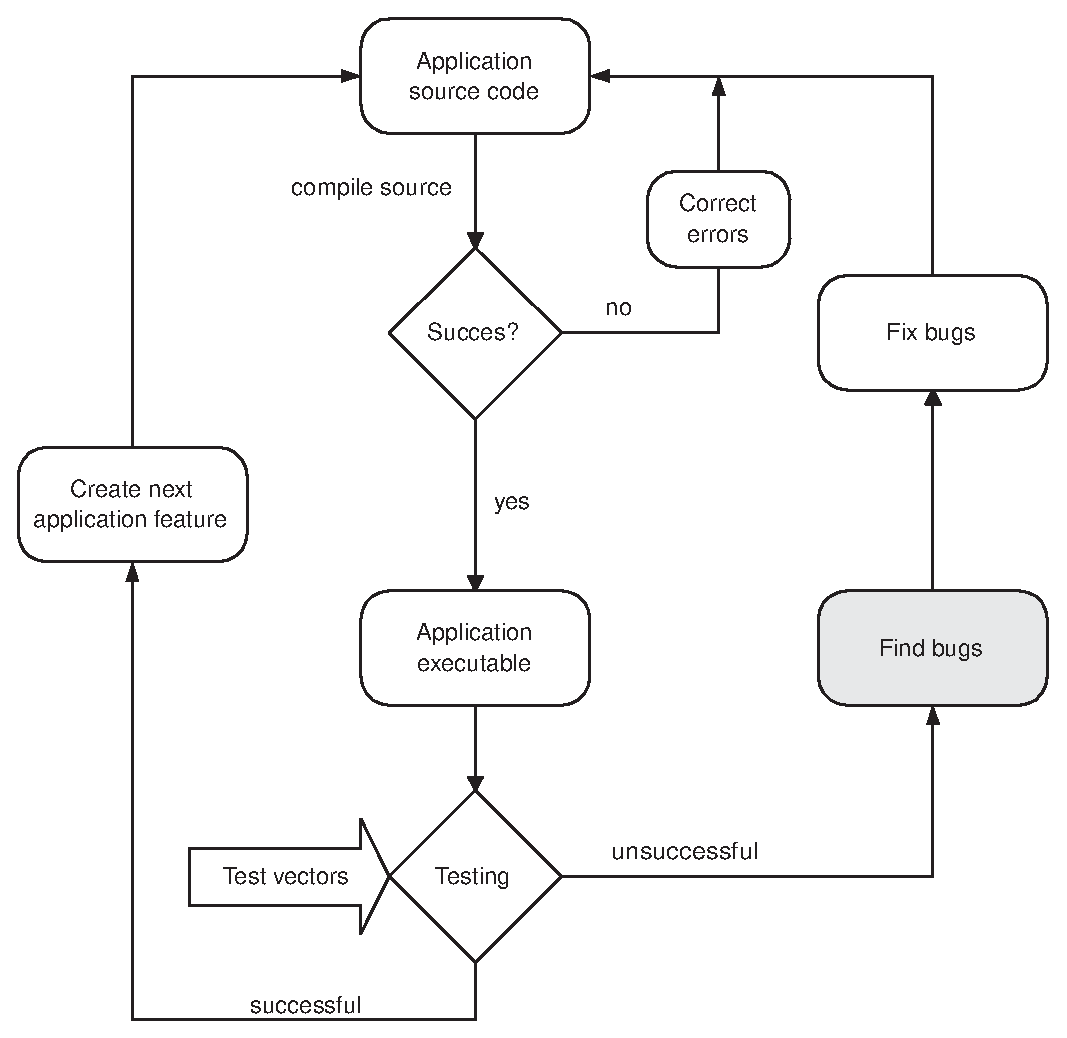
\includegraphics[width=10cm]{./figures/testcycle.eps}
\caption{The test -- debug -- develop cycle}
\label{fig:testing:cycle}
\end{center} \end{figure}

%%% Nick seemed to like this very much (001208)
\section{Debug techniques used} \label{chap:testing:techniques}
The best technique to find a bug depends on the type of bug encountered. The
bugs encountered most are:
\begin{itemize}
\item Unexpected behaviour. The application does not perform its task correctly
or not all.
\item Segmentation faults/bus errors. The application ``crashes''. Segmentation faults are usually due to
an abused pointer.
\item Crashes or unexpected behaviour associated with signals/slots.
\end{itemize}
Useful approaches for finding the location (or reason) for these bugs will be
discussed next.

\subsection{Unexpected behaviour}
An example of unexpected behaviour could be the erroneous generation of the
text resulting from the \verb=foreach= loops in the configuration file. The
algorithm was either not correct or not correctly implemented. To ascertain the
exact location or reason for this bug it necessary to gain more insight into
how the algorithm is ``run''.

The best way to gain insight into the inner workings of an algorithm is by
using a debugger. An excellent debugger is \verb=gdb=. Unfortunately, it has no
graphical front end. This means some experience is required to use \verb=gdb=
effectively. It is therefore recommended to use a graphical front-end to
\verb=gdb= like \verb=DDD= (the Data Display Debugger), \verb=xgdb= or even \verb=xemacs=.
Another option is \verb=kdbg=. These debuggers allow step-by-step execution of
the source code and inspection of the values of the variables used.


\bigskip \noindent
Another useful method could be to use debug statements. These print out
information about the state of the application at strategic places. If a smart
\verb=#define= statement is used it is possible to disable the output for
release builds.

\subsection{Locating segmentation faults}
Contrary to unexpected behaviour, segmentation faults can be located quite
easily. If the application is run from the debugger it will report the location
the segmentation fault occurred. In \verb=gdb= this can be done with the
backtrace command \verb=bt=. This lists a backtrace of the stack, showing
exactly how the application reached the point where the segmentation fault
occurred.

Once the location of the segmentation fault is known the reason for it is
usually (but not always) clear and fixing the bug can begin.

\subsection{Signal/slot debugging}
The signal/slot mechanism provided by Qt presents a challenge in case of bugs.
Segmentation faults that occur right after a signal can be extremely difficult
to locate or solve.

The signal/slot mechanism is available to any class that inherits the
\verb=QObject= class. This includes all widgets. If a backtrace of the stack is
requested right after a segmentation fault it will only display methods used by
these Qt objects. It is very difficult to pinpoint the exact object that sent
the signal (and often caused the error).

\paragraph{A common signal/slot pitfall\\ }
An error often made that is difficult to find is the deletion of the sending
object from the receiving slot. For example, object \verb=A= sends a signal to
object \verb=B=. Because of this signal, \verb=B= tells the manager of \verb=A=
objects \verb=C= to delete certain \verb=A= objects. If one of these \verb=A=
objects was the object that originally sent the message a segmentation fault is
very likely.

The reason for this is the fact that emitting a signal is nothing more than
calling a method. Once the signal method completes it will eventually return to
the place the signal was emitted. If that object has been deleted this location
is no longer valid and a segmentation fault will occur.

For more insights into how the signal/slot mechanism is implemented the
interested user is recommend to take a look at the output of the
\verb=meta object compiler= and the source of the \verb=QObject= class.

\bigskip \noindent
\paragraph{Tips\\}
Some additional tips:
\begin{itemize}
\item Compile Qt with debugging on and use this library during development.
Warnings about unconnected signals/slots will then be issued by Qt. It is also
possible to dump information about a \verb=QObject= tree.
\item The meta object compiler \verb=moc= also has a debugging feature.
Enabling this feature can be useful to track signals/slots.
\end{itemize}

%% background.tex
%
%
\chapter{About SPACE and the ocean package}
\label{chap:background}


% cdrom.tex

\chapter{About the CD-ROM}
\label{chap:cdrom}

The CD-ROM accompanying this report contains the results of the project. The
table below lists the locations of everything on the CD-ROM.

\begin{tabularx}{\textwidth}{X|X}
 \hline
 \textsf{Location} & Description \\
 \hline
 \texttt{binaries\(\backslash\)examples} & Contains sample processes for use with the application. \\
 \texttt{binaries\(\backslash\)Linux} & Contains binaries for Linux \\
 \texttt{binaries\(\backslash\)Solaris} & Contains binaries for Solaris \\
 \texttt{cvs\_repository} & Contains the CVS repository used during the development of the application. \\
 \texttt{documentation\(\backslash\)nonpostscript pictures} & Contains non-postscript versions of the pictures used in this thesis. \\
 \texttt{documentation\(\backslash\)paper} & Contains the \LaTeX source of the  paper written for this project. \\
 \texttt{documentation\(\backslash\)source code} & Contains the source code documentation \\
 \texttt{documentation\(\backslash\)source code} & Contains the \LaTeX source of  this thesis. \\
 \texttt{presentation} & Contains files used for the presentation. \\
 \texttt{spock} & Contains the sources of the application. \\
 \hline
\end{tabularx}

% samplespock.tex

\chapter{A sample configuration file} \label{chapt:samplespock}

Below a sample configuration file is given. To save some trees, the example is
a \emph{part} of an early configuration file created during development of the
application. Many of the language constructions are put into action so it makes
a nice example.

\begin{alltt}
\tiny
// This is a SPOCK version 1.0 user interface specification...
//
//////////////////////////////////////////////////////////////////////////////
// Please do not "just" change this file. You could seriously break
// the spock program. Only edit this file if you know what actions
// will brake compatibility with your saved processes.
// For more information, please refer to the SPOCK source code documentation
// or Xander Burgerhout's graduation report.
//
// Consider this file as part of the source.
//
// !!YOU HAVE BEEN WARNED!!
//////////////////////////////////////////////////////////////////////////////

//////////////////////////////////////////////////////////////////////////////
// Icon path.
// The icon (pixmap) path specifies where pixmap(...) properties look for the
// icons.
ICONPATH = "$(ICDPATH)/lib/spock"

//////////////////////////////////////////////////////////////////////////////
// Defines.
define dropdown layer \{
    adddatafrom(maskdata_sheet.name);
\}

define combobox layer_combo \{
    adddatafrom(maskdata_sheet.name);
\}

define dropdown layer_gnd \{
    item atgnd \{ title("@gnd"); \}
    adddatafrom(maskdata_sheet.name);
\}

define dropdown layer_sub \{
    item atsub \{ title("@sub"); \}
    adddatafrom(maskdata_sheet.name);
\}

define dropdown layer_gndsub \{
    item atsub \{ title("@sub"); \}
    item atgnd \{ title("@gnd"); \}
    adddatafrom(maskdata_sheet.name);
\}

// Defines a carrier type
define combobox def_carr_type \{
    item n \{ title("n doped conductor"); \}
    item p \{ title("p doped conductor"); \}
    item m \{ title("metal"); \}
    default(m);
\}

// Defines a transistor type
define dropdown def_trans_type \{
    item ver \{ title("vertical"); \}
    item lat \{ title("lateral"); \}
    default(ver);
\}

define dropdown def_layer_type \{
    item normal \{ title("normal"); \}
    item interconnect \{ title("interconnect"); \}
    item symbolic \{ title("symbolic"); \}
    default(normal);
\}

define conditionlist condlist_simp \{
    option("noextended");
    adddatafrom(maskdata_sheet.name, maskdata_sheet.comment);
\}

define conditionlist condlist_ext \{
    option("extended");
    adddatafrom(maskdata_sheet.name, maskdata_sheet.comment);
\}

define dropdown capa_types \{
    item normal \{ title("default"); \}
    item junction \{ title("junction"); \}
    default(normal);
\}


//////////////////////////////////////////////////////////////////////////////
// Element definition user interface specification.
//
// This part consists mostly of sections. In the tabpages part of this file,
// these sections are used to create the element definition tabpage.

section units \{
    title("Unit specification");
    hint("Use this to specify a base for the values you enter");
    pixmap("section_icons/units.xpm");

    paramlist units_list \{
        real resistance \{
            title("Sheet resistance unit:");
            unit("in ohm");
            hint("You can specify a base for the values you\(\backslash\)n"
                 "will enter below. Use as follows:\(\backslash\)n"
                 "If you do not want to type 3e-6, 8e-6 12.5e-6, etc.\(\backslash\)n"
                 "but 3, 8, 12.5 instead, type 1e-6 here.");
        \}
        real c_resistance \{
            title("Contact resistance unit:");
            unit("in ohm per squared meter");
        \}
        real a_capacitance \{
            title("Area capacitance unit:");
            unit("in farad per squared meter");
        \}
        real e_capacitance \{
            title("Edge or lateral capacitance unit:");
            unit("in farad per meter");
        \}
        real distance \{
            title("Capacitance unit:");
            unit("in micron");
        \}

        // This is for Space 3D
        real vdimension \{
            title("Vertical dimension unit:");
            unit("in micron");
        \}

        real shape \{
            title("Edge shape list dimension unit:");
            unit("in micron");
        \}
    \}
\}

section conductors \{
    title("Conductor list");
    hint ("Definitions for the conducting layers in the circuit");
    pixmap("section_icons/conductor.xpm");

    spreadsheet conductors_sheet \{
        identifier      cond_type \{ title("Conductor type"); \}
        identifier      name \{ title("Name"); \}
        condlist_simp   cond_list \{ title("Condtion list"); \}
        layer           mask \{ title("Mask"); \}
        real            sheet_res \{
                            title("Sheet resistivity");
                            align(right);
                        \}
        def_carr_type   carr_type \{ title("Carrier type"); \}
        string          comment \{ title("Comment"); \}
    \}
\}

section fets \{
    title("Field-effect transistor (FET) list");
    hint("FET definitions");
    pixmap("section_icons/fet.xpm");

    spreadsheet fets_sheet \{
        identifier      name \{ title("Name"); \}
        condlist_simp   cond_list \{ title("Condtion list"); \}
        layer           mask_g \{ title("Gate mask"); \}
        layer           mask_ds \{ title("Drain/source mask"); \}
        layer_sub       mask_b \{ title("Bulk mask"); \}
        string          comment \{ title("Comment"); \}
    \}
\}

section bjts \{
    title("Bipolar transistor list");
    pixmap("section_icons/bipolar.xpm");

    spreadsheet bjts_sheet \{
        identifier      name \{ title("Name"); \}
        condlist_ext    cond_list \{ title("Condtion list"); \}
        def_trans_type  ttype \{ title("Transistor type"); \}
        layer           mask_em \{ title("Emitter mask"); \}
        layer           mask_ba \{ title("Base mask"); \}
        layer           mask_co \{ title("Collector mask"); \}
        string          comment \{ title("Comment"); \}
    \}
\}

section connects \{
    title("Connect list");
    pixmap("section_icons/connect.xpm");

    spreadsheet connects_sheet \{
        identifier      name \{ title("Name"); \}
        conditionlist   cond_list \{ title("Condtion list"); \}
        layer           mask_1 \{ title("Mask 1"); \}
        layer           mask_2 \{ title("Mask 2"); \}
        string          comment \{ title("Comment"); \}
    \}
\}

section contacts \{
    title("Contact list");
    pixmap("section_icons/contact.xpm");

    spreadsheet contacts_sheet \{
        identifier      contact_type \{ title("Contact type"); \}
        identifier      name \{ title("Name"); \}
        condlist_simp   cond_list \{ title("Condtion list"); \}
        layer_sub       mask_1 \{ title("Mask 1"); \}
        layer_sub       mask_2 \{ title("Mask 2"); \}
        real            resistivity \{ title("Resistivity"); \}
        string          comment \{ title("Comment"); \}
    \}
\}

section capacitances \{
    title("Capacitance list");
    pixmap("section_icons/capacitance.xpm");

    spreadsheet cap_sheet \{
        capa_types      cap_type \{ title("Type"); \}
        identifier      subtype \{ title("Sub type"); \}
        identifier      name \{ title("Name"); \}
        condlist_ext    cond_list \{ title("Condtion list"); \}
        layer           mask_1 \{ title("Mask 1"); \}
        layer           mask_2 \{ title("Mask 2"); \}
        string          capacitivity \{ title("Capacitivity"); \}
        string          comment \{ title("Comment"); \}
    \}
\}

/////////////////////////////////////////////////
// Maskdata specification

section maskdata_info \{
    title("Layers");
    pixmap("section_icons/layers.xpm");

    spreadsheet maskdata_sheet \{
        integer[0..10]     ID \{ title("Layer ID"); \}
        identifier          name \{ title("Layer name"); \}
        def_layer_type      layertype \{ title("Layer type"); \}
        dalistyle           dali \{ title("Dali draw style"); \}
        color               xspace \{ title("XSpace draw color"); \}
        string              comment \{ title("Comment"); \}
    \}
\}

//////////////////////////////////////////////////
// Space parameters
section space_params_section \{
    title("Space parameters");

    paramlist space_params \{
        integer min_art_degree \{
            title("Minimal articulation degree");
            hint("The articulation degree is the number of pieces in which\(\backslash\)n"
                  "the resistance graph would break if the node and its \(\backslash\)n"
                  "connected resistances were removed");
            default("3");
        \}
        integer min_degree \{
            title("Minimal degree");
            hint("Nodes with a degree >= this value and an articulation\(\backslash\)n"
                 "degree > 1 will also be retained in the final network.");
            default("4");
        \}
        real min_res \{
            title("Minimal resistance");
            unit("ohm");
            hint("This heuristic deletes small resistances from the network\(\backslash\)n"
                  "via Gaussian elimination of one of the nodes that is\(\backslash\)n"
                  "connected to the resistance.");
            default("100");
        \}
        real min_sep_res \{
            title("Minimal separation resistance");
            unit(ohm);
            hint("This heuristic deletes small resistances from the network\(\backslash\)n"
                 "by joining the two nodes that are connected by the resistance.");
            default("10");
        \}
        real max_par_res \{
            title("Maximal parallel resistance");
            unit("ohm");
            hint("This heuristic prevents the occurance of high-ohmic shunt\(\backslash\)n"
                 "paths between two nodes.");
            default("25");
        \}

        // no_neg_res comes here.

        real min_coup_cap \{
            title("Minimal coupling capacitance ratio");
            hint("If, for both nodes a coupling capacitance is connected to,\(\backslash\)n"
                 "it holds that the ratio between the absolute value of the\(\backslash\)n"
                 "coupling capacitance and the value of the ground/substrate\(\backslash\)n"
                 "capacitance of the same type of that node, is less than this\(\backslash\)n"
                 "parameter, then the value of the coupling capacitance is \(\backslash\)n"
                 "added to the ground capacitances of the two nodes and the\(\backslash\)n"
                 "coupling capacitance is removed.");
            default("0.04");
        \}
    \}
\}

//////////////////////////////////////////////////
// Getepslay

define dropdown term_text_align \{
    item al_00   \{ title("Center of text at center of terminal"); \}
    item al_n10  \{ title("Left-hand of text at center of terminal"); \}
    item al_10   \{ title("Right-hand of text at center of terminal"); \}
    item al_01   \{ title("Text centered below center of terminal"); \}
    item al_0n1  \{ title("Text centered above center of terminal"); \}
    default(al_00);
\}

section getepslay_preamble \{
    title("General settings");
    paramlist getepslay_pl \{
        string includefile_nelsis \{
            title("Include file from nelsis");
            hint("Includes a postscript prolog file.\(\backslash\)n"
                 "The filename given must be relative to $NELSISHOME/lib/\(\backslash\)n"
                 "NOTE: only one level of inclusion is supported.");
            default("epslay.pro");
        \}
        string includefile_home \{
            title("Include file from home directory");
            hint("Includes a postscript prolog file.\(\backslash\)n"
                 "The filename given must be relative to the home directory."
                 "NOTE: only one level of inclusion is supported.");
            default("");
        \}
        string mask_order \{
            title("Mask draw order");
            hint("Specify in which order the masks must be drawn.\(\backslash\)n");
        \}
        string plotfont \{
            title("Font for terminal names");
            hint("Any available PostScript font is acceptable.");
            default("Helvetica-Bold");
        \}
        integer font_min \{
            title("Minimum text size");
            unit("1/72 inch");
            hint("Minimum size of text in printer's points");
            default("6");
        \}
        integer font_max \{
            title("Maximum text size");
            unit("1/72 inch");
            hint("Maximum size of text in printer's points");
            default("14");
        \}
        integer font_lambda \{
            title("Preferred size of text in lambda's");
            unit("lambda's");
            hint("Based on the scaling of the particular layout in order to\(\backslash\)n"
                 "fill the drawing region, the text size is first computed\(\backslash\)n"
                 "according to this value. Then, the min and max values\(\backslash\)n"
                 "above are applied.\(\backslash\)n"
                 "A value approximately equal to the size of contact windows\(\backslash\)n"
                 "is often appropiate.");
        \}
        real pattern_scale \{
            title("Global stipple pattern magnification");
            unit("x");
            hint("Globally magnify the scale of the stipple pattern\(\backslash\)n"
                 "by the factor given here. Integral values work best.\(\backslash\)n"
                 "Often useful for rendering on low resolution devices.");
            default("1");
        \}

        term_text_align termtxt \{
            title("Terminal name alignment");
            hint("Specifies the aligment of the terminal names with\(\backslash\)n"
                 "respect to the center of the terminal");
        \}
    \}
\}

section getepslay_body \{
    title("Individual mask plotting styles");

    spreadsheet getepslay_sheet \{
        layer_combo mask_name \{ title("Mask"); \}
        string      pattern \{ title("Pattern"); \}
        real        scale \{ title("Scale"); default("1.0"); \}
        real        linewidth \{ title("Linewidth in lambda's"); \}
    \}
\}



//////////////////////////////////////////////////
// Tabpages
tabpage element_def_tab \{
    title("Element definition");
    scrollframe element_def \{
        section maskdata_info;
        section units;
        section conductors;
        section fets;
        section bjts;
        section connects;
        section contacts;
        section capacitances;
    \}
\}

tabpage space_parameters_tab \{
    title("Space parameters");
//    multi_section space_param_frame \{
        section space_params_section;
//    \}
\}

tabpage getepslay_tab \{
    title("Postscript plot settings");
    scrollframe getepslay_frame \{
        section getepslay_preamble;
        section getepslay_body;
    \}
\}

//////////////////////////////////////////////////
// Generators

generator maskdata_gen
\{
    filename("maskdata");
    title("Maskdata file");

    map def_carr_type \{
        n = "n";
        p = "p";
        m = "m";
    \}

    map def_layer_type \{
        normal       = "0";
        interconnect = "1";
        symbolic     = "2";
    \}

    generate \{
        "## This file was generated by SPOCK on " application[date]
        " at " application[time] ".\(\backslash\)n"
        "#-----------------------------------------------------------------------------\(\backslash\)n"
        "#\(\backslash\)n"
        "#                       M A S K D A T A   I N F O\(\backslash\)n"
        "#\(\backslash\)n"
        "#       Layer fields (3):       field  1: layer number\(\backslash\)n"
        "#                               field  2: layer name\(\backslash\)n"
        "#                               field  3: layer type\(\backslash\)n"
        "#                                         type = 0: normal layer\(\backslash\)n"
        "#                                         type = 1: interconnect layer\(\backslash\)n"
        "#                                                   (terminals/labels may be\(\backslash\)n"
        "#                                                    defined for this layer).\(\backslash\)n"
        "#                                         type = 2: symbolic layer\(\backslash\)n"
        "#\(\backslash\)n"
        "#       Pattern-Generate (2):   field  4: job number\(\backslash\)n"
        "#       Only used by PG-tape    field  5: mask type\(\backslash\)n"
        "#       programs                          type = 0: negative\(\backslash\)n"
        "#                                         type = 1: positive\(\backslash\)n"
        "#\(\backslash\)n"
        "#       ColorMask Terminals (2) field  6: color number\(\backslash\)n"
        "#       (Obsolete)              field  7: fill style\(\backslash\)n"
        "#\(\backslash\)n"
        "#       (Sea)Dali (2)           field  8: color number\(\backslash\)n"
        "#                                         0=black, 1=red, 2=green,\(\backslash\)n"
        "#                                         3=yellow, 4=blue, 5=violet,\(\backslash\)n"
        "#                                         6=aqua, 7=white\(\backslash\)n"
        "#                               field  9: fill style\(\backslash\)n"
        "#                                         0=hashed, 1=solid, 2=hollow\(\backslash\)n"
        "#                                         3,4,5 = 12,25,50% hash+outline\(\backslash\)n"
        "#                                         6,7,8 = idem, no outline\(\backslash\)n"
        "#\(\backslash\)n"
        "#       Plotter (2)             field 10: pen number\(\backslash\)n"
        "#       (Obsolete)                        1=black, 2=red, 3=yellow,\(\backslash\)n"
        "#                                         4=green, 5=brown, 6=violet,\(\backslash\)n"
        "#                                         7=blue, 8=aqua\(\backslash\)n"
        "#                               field 11: fill style\(\backslash\)n"
        "#\(\backslash\)n#\(\backslash\)n"

        maskdata_sheet[numrows]
        " \(\backslash\)"" application[processname] "\(\backslash\)" \(\backslash\)"" application[processdesc] "\(\backslash\)"\(\backslash\)n"
        "# ID\(\backslash\)tname\(\backslash\)ttype\(\backslash\)tPG_tape CM\(\backslash\)tDali\(\backslash\)tplot  comment\(\backslash\)n"

        foreach(maskdata_sheet, row) \{
            ID
            "\(\backslash\)t" name "\(\backslash\)t"
            layertype
            "\(\backslash\)t1 0     1 0\(\backslash\)t"
            dali[clr] " "
            dali[style]
            "\(\backslash\)t1 0   \(\backslash\)""
            comment
            "\(\backslash\)"\(\backslash\)n"
        \}
    \}
\}

generator space_def_s_gen
\{
    filename("space.def.s");
    title("SPACE Element definition file");

    map def_carr_type \{
        n = "n";
        p = "p";
        m = "m";
    \}

    generate \{

        "## This file was generated by SPOCK on " application[date]
        " at " application[time] ".\(\backslash\)n"
        "#####\(\backslash\)n"
        "# " application[processname] " - " application[processdesc] "\(\backslash\)n"

        "#\(\backslash\)n# Masks:\(\backslash\)n"
        foreach(maskdata_sheet, row) \{
            "# " name "\(\backslash\)t" comment "\(\backslash\)n"
        \}
        "# See also the maskdata file.\(\backslash\)n"
        "#####\(\backslash\)n"

        "unit resistance    "   units.units_list.resistance "\(\backslash\)t# ohm\(\backslash\)n"
        "unit c_resistance  "   units.units_list.c_resistance "\(\backslash\)t# ohm/m^2\(\backslash\)n"
        "unit a_capaictance "   units_list.a_capacitance "\(\backslash\)t# F/m^2\(\backslash\)n"
        "unit e_capacitance "   units_list.e_capacitance "\(\backslash\)t# F/m\(\backslash\)n"
        "unit distance      "   units_list.distance "\(\backslash\)t# micron\(\backslash\)n"
        "unit vdimension    "   units_list.vdimension "\(\backslash\)t# micron\(\backslash\)n"
        "unit shape         "   units_list.shape "\(\backslash\)t# micron\(\backslash\)n\(\backslash\)n"

        "colors:\(\backslash\)n"
         foreach(maskdata_sheet, row) \{
            "\(\backslash\)t" name "\(\backslash\)t" xspace "\(\backslash\)n"
         \}
         "\(\backslash\)n"

         foreach $t (conductors_sheet, cond_type) \{
             "conductors " $t ":\(\backslash\)n"
             "  # name:condition_list:mask:sheet_resistivity:carrier_type\(\backslash\)n"
             foreach(conductors_sheet, row) \{
                if (cond_type == $t) \{
                    "\(\backslash\)t" name ":" cond_list ":" mask ":" sheet_res ":" carr_type "\(\backslash\)t\(\backslash\)t# " comment "\(\backslash\)n"
                \}
             \}
             "\(\backslash\)n"
         \}

         "fets:\(\backslash\)n"
         "#\(\backslash\)tname:condition list:mask_g mask_ds:mask_b\(\backslash\)n"
         foreach(fets.fets_sheet, row) \{
            "\(\backslash\)t" name ":" cond_list ":" mask_g " " mask_ds ":" mask_b "\(\backslash\)t\(\backslash\)t# " comment "\(\backslash\)n"
         \}
         "\(\backslash\)n"

         "bjts:\(\backslash\)n"
         "#\(\backslash\)tname:condition_list:type:mask_em mask_ba mask_co\(\backslash\)n"
         foreach(bjts.bjts_sheet, row) \{
            "\(\backslash\)t" name ":" cond_list ":" ttype ":" mask_em " " mask_ba " " mask_co "\(\backslash\)t\(\backslash\)t# " comment "\(\backslash\)n"
         \}
         "\(\backslash\)n"

         "connects:\(\backslash\)n"
         "#\(\backslash\)tname:condition_list:type:mask1 mask2\(\backslash\)n"
         foreach(connects.connects_sheet, row) \{
            "\(\backslash\)t" name ":" cond_list ":" mask_1 " " mask_2 "\(\backslash\)t\(\backslash\)t# " comment "\(\backslash\)n"
         \}
         "\(\backslash\)n"

         foreach $t (contacts_sheet, contact_type) \{
             "contacts " $t ":\(\backslash\)n"
             "#\(\backslash\)tname:condition_list:type:mask1 mask2:resitivity\(\backslash\)n"
             foreach(contacts.contacts_sheet, row) \{
                if (contact_type == $t) \{
                    "\(\backslash\)t" name ":" cond_list ":" mask_1 " " mask_2 ":" resistivity "\(\backslash\)t\(\backslash\)t# " comment "\(\backslash\)n"
                \}
             \}
             "\(\backslash\)n"
         \}

         foreach $t (cap_sheet, cap_type) \{
            foreach $s (cap_sheet, subtype) \{
                 $t " capacitances " $s ":\(\backslash\)n"
                 "#\(\backslash\)tname:condition_list:type:mask1 [mask2]:capacitivity\(\backslash\)n"
                 foreach(capacitances.cap_sheet, row) \{
                    if (cap_type == $t) \{
                        if (subtype == $s) \{
                            "\(\backslash\)t" name ":" cond_list ":" mask_1 " " mask_2 ":" capacitivity "\(\backslash\)t\(\backslash\)t# " comment "\(\backslash\)n"
                        \}
                    \}
                 \}
                 "\(\backslash\)n"
            \}
         \}

        ////////////////////////////
        // This is for space3d only

        "vdimensions:\(\backslash\)n"
         "#\(\backslash\)tname:condition_list:mask:bottom thickness\(\backslash\)n"
         foreach(vdimensions_sheet, row) \{
            "\(\backslash\)t" name ":" cond_list ":" mask ":" bottom " " thickness "\(\backslash\)t# " comment "\(\backslash\)n"
         \}
         "\(\backslash\)n"

        "eshapes:\(\backslash\)n"
        "\(\backslash\)t#name:condition_list:mask:dxb dxt\(\backslash\)n"
        foreach(eshapes_sheet, row) \{
            "\(\backslash\)t" name ":" cond_list ":" mask ":" dxb " " dxt "\(\backslash\)t# " comment "\(\backslash\)n"
        \}
        "\(\backslash\)n"

        "dielectrics:\(\backslash\)n"
        "\(\backslash\)t#name permittivity bottom\(\backslash\)n"
        foreach(dielectrics_sheet, row) \{
            "\(\backslash\)t" name " " permittivity " " bottom "\(\backslash\)t# " comment "\(\backslash\)n"
        \}

    \}
\}

generator space_param_gen
\{
    filename("space.def.p");
    title("SPACE parameter file");

    generate \{
        "## This file was generated by SPOCK on " application[date]
        " at " application[time] ".\(\backslash\)n"
        "#####\(\backslash\)n"
        "# SPACE parameter file for " application[processname] " - " application[processdesc] "\(\backslash\)n"
        "#####################################################################\(\backslash\)n\(\backslash\)n"

        if (space_params.min_art_degree != "") \{
            "min_art_degree      " space_params.min_art_degree "\(\backslash\)n"
        \}

        if (space_params.min_degree != "") \{
            "min_degree          " space_params.min_degree "\(\backslash\)n"
        \}

        if (space_params.min_res != "") \{
            "min_res             " space_params.min_res "\(\backslash\)t# ohm\(\backslash\)n"
        \}

        if (space_params.min_sep_res != "") \{
            "min_sep_res         " space_params.min_sep_res "\(\backslash\)t# ohm\(\backslash\)n"
        \}

        if (space_params.max_par_res != "") \{
            "min_par_res         " space_params.max_par_res "\(\backslash\)n"
        \}

        if (space_params.min_coup_cap != "") \{
            "min_coup_cap      " space_params.min_coup_cap "\(\backslash\)n"
        \}
    \}
\}

generator getepslay_gen \{
    title("Getepslay PostScript settings");
    filename("epslay.def");

    map term_text_align \{
        al_00   = "0 0";
        al_n10  = "-1 0";
        al_10   = "1 0";
        al_01   = "0 1";
        al_0n1  = "0 -1";
    \}

    generate \{
        "%% This file was generated by SPOCK on " application[date] " at " application[time] ".\(\backslash\)n"
        "%% getepslay customization for the " application[processname] " process.\(\backslash\)n\(\backslash\)n"

        if (getepslay_pl.includefile_nelsis != "") \{
            "%%Include <" getepslay_pl.includefile_nelsis ">\(\backslash\)n"
        \}
        if (getepslay_pl.includefile_home != "") \{
            "%%Include \(\backslash\)"" getepslay_pl.includefile_nelsis "\(\backslash\)"\(\backslash\)n"
        \}
        "\(\backslash\)n"
        "%%Order: " getepslay_pl.mask_order "\(\backslash\)n"
        "[ " getepslay_pl.font_min " " getepslay_pl.font_max " " getepslay_pl.font_lambda
        "/" getepslay_pl.plotfont " ] plotFont\(\backslash\)n"
        "[ " getepslay_pl.termtxt " ] termTextAlignment\(\backslash\)n\(\backslash\)n"


        "% mask\(\backslash\)tpattern\(\backslash\)tscale\(\backslash\)tlinewidth\(\backslash\)n"
        foreach (getepslay_sheet, row) \{
            "[ (" mask_name ")\(\backslash\)t" pattern "\(\backslash\)t" scale "\(\backslash\)t" linewidth " ] defineStyle\(\backslash\)n"
        \}
    \}
\}

\end{alltt}

%% sourceref.tex

%% Doxygen generated source code reference.

%\chapter{Source code reference}
%\label{chap:sourceref}

%%% The source code reference is too large to include...


\end{document}

